\documentclass[twoside]{article}

% Packages required by doxygen
\usepackage{calc}
\usepackage{doxygen}
\usepackage{graphicx}
\usepackage[utf8]{inputenc}
\usepackage{makeidx}
\usepackage{multicol}
\usepackage{multirow}
\usepackage{textcomp}
\usepackage[table]{xcolor}

% Font selection
\usepackage[T1]{fontenc}
\usepackage{mathptmx}
\usepackage[scaled=.90]{helvet}
\usepackage{courier}
\usepackage{amssymb}
\usepackage{sectsty}
\renewcommand{\familydefault}{\sfdefault}
\allsectionsfont{%
  \fontseries{bc}\selectfont%
  \color{darkgray}%
}
\renewcommand{\DoxyLabelFont}{%
  \fontseries{bc}\selectfont%
  \color{darkgray}%
}

% Page & text layout
\usepackage{geometry}
\geometry{%
  a4paper,%
  top=2.5cm,%
  bottom=2.5cm,%
  left=2.5cm,%
  right=2.5cm%
}
\tolerance=750
\hfuzz=15pt
\hbadness=750
\setlength{\emergencystretch}{15pt}
\setlength{\parindent}{0cm}
\setlength{\parskip}{0.2cm}
\makeatletter
\renewcommand{\paragraph}{%
  \@startsection{paragraph}{4}{0ex}{-1.0ex}{1.0ex}{%
    \normalfont\normalsize\bfseries\SS@parafont%
  }%
}
\renewcommand{\subparagraph}{%
  \@startsection{subparagraph}{5}{0ex}{-1.0ex}{1.0ex}{%
    \normalfont\normalsize\bfseries\SS@subparafont%
  }%
}
\makeatother

% Headers & footers
\usepackage{fancyhdr}
\pagestyle{fancyplain}
\fancyhead[LE]{\fancyplain{}{\bfseries\thepage}}
\fancyhead[CE]{\fancyplain{}{}}
\fancyhead[RE]{\fancyplain{}{\bfseries\leftmark}}
\fancyhead[LO]{\fancyplain{}{\bfseries\rightmark}}
\fancyhead[CO]{\fancyplain{}{}}
\fancyhead[RO]{\fancyplain{}{\bfseries\thepage}}
\fancyfoot[LE]{\fancyplain{}{}}
\fancyfoot[CE]{\fancyplain{}{}}
\fancyfoot[RE]{\fancyplain{}{\bfseries\scriptsize Generated on Mon Jun 2 2014 13\-:59\-:31 for Super Martin Level Editor by Doxygen }}
\fancyfoot[LO]{\fancyplain{}{\bfseries\scriptsize Generated on Mon Jun 2 2014 13\-:59\-:31 for Super Martin Level Editor by Doxygen }}
\fancyfoot[CO]{\fancyplain{}{}}
\fancyfoot[RO]{\fancyplain{}{}}
\renewcommand{\footrulewidth}{0.4pt}
\renewcommand{\sectionmark}[1]{%
  \markright{\thesection\ #1}%
}

% Indices & bibliography
\usepackage{natbib}
\usepackage[titles]{tocloft}
\setcounter{tocdepth}{3}
\setcounter{secnumdepth}{5}
\makeindex

% Hyperlinks (required, but should be loaded last)
\usepackage{ifpdf}
\ifpdf
  \usepackage[pdftex,pagebackref=true]{hyperref}
\else
  \usepackage[ps2pdf,pagebackref=true]{hyperref}
\fi
\hypersetup{%
  colorlinks=true,%
  linkcolor=blue,%
  citecolor=blue,%
  unicode%
}

% Custom commands
\newcommand{\clearemptydoublepage}{%
  \newpage{\pagestyle{empty}\cleardoublepage}%
}


%===== C O N T E N T S =====

\begin{document}

% Titlepage & ToC
\hypersetup{pageanchor=false}
\pagenumbering{roman}
\begin{titlepage}
\vspace*{7cm}
\begin{center}%
{\Large Super Martin Level Editor }\\
\vspace*{1cm}
{\large Generated by Doxygen 1.8.6}\\
\vspace*{0.5cm}
{\small Mon Jun 2 2014 13:59:31}\\
\end{center}
\end{titlepage}
\tableofcontents
\pagenumbering{arabic}
\hypersetup{pageanchor=true}

%--- Begin generated contents ---
\section{Data Structure Documentation}
\hypertarget{struct_cursor}{\section{Cursor Struct Reference}
\label{struct_cursor}\index{Cursor@{Cursor}}
}
\subsection*{Data Fields}
\begin{DoxyCompactItemize}
\item 
\hypertarget{struct_cursor_a6150e0515f7202e2fb518f7206ed97dc}{int {\bfseries x}}\label{struct_cursor_a6150e0515f7202e2fb518f7206ed97dc}

\item 
\hypertarget{struct_cursor_a0a2f84ed7838f07779ae24c5a9086d33}{int {\bfseries y}}\label{struct_cursor_a0a2f84ed7838f07779ae24c5a9086d33}

\item 
\hypertarget{struct_cursor_aeeda4ec0cbb14f14167705f44156e13e}{int {\bfseries tile\-I\-D}}\label{struct_cursor_aeeda4ec0cbb14f14167705f44156e13e}

\end{DoxyCompactItemize}


The documentation for this struct was generated from the following file\-:\begin{DoxyCompactItemize}
\item 
\hyperlink{const_8h}{const.\-h}\end{DoxyCompactItemize}

\hypertarget{struct_input}{\subsection{Input Struct Reference}
\label{struct_input}\index{Input@{Input}}
}


{\ttfamily \#include $<$input.\-h$>$}

\subsubsection*{Data Fields}
\begin{DoxyCompactItemize}
\item 
char \hyperlink{struct_input_afc4eabd057bd0061b56de4005f5ecbb8}{key} \mbox{[}S\-D\-L\-K\-\_\-\-L\-A\-S\-T\mbox{]}
\item 
int \hyperlink{struct_input_ab05991ed532329184893692211b355fa}{space}
\item 
int \hyperlink{struct_input_a2896431d6a80cd39b3d24b40237612ee}{quit}
\item 
int \hyperlink{struct_input_a163e08d0d19093f658f448710f8e3c49}{is\-Joystick}
\item 
int \hyperlink{struct_input_a66b84ad51037935b993fc2b860b15cb6}{use\-Joystick}
\item 
S\-D\-L\-\_\-\-Joystick $\ast$ \hyperlink{struct_input_a5fe6c6b426f70a21df07c64227b2c337}{joystick}
\item 
char $\ast$ \hyperlink{struct_input_a7f901d4dc1179ea534cb9e5cce0a260b}{button}
\item 
int $\ast$ \hyperlink{struct_input_ae2fe71f7c5edeaa9fc2676be4a93499a}{axes}
\item 
int $\ast$ \hyperlink{struct_input_ab1c8c264ad7cfee584093b1479c03f75}{hat}
\item 
int \hyperlink{struct_input_af7cf3c53ae2105eec18ce989dd3ddae0}{hat\-Moved}
\end{DoxyCompactItemize}


\subsubsection{Detailed Description}
the global input structure 

\subsubsection{Field Documentation}
\hypertarget{struct_input_ae2fe71f7c5edeaa9fc2676be4a93499a}{\index{Input@{Input}!axes@{axes}}
\index{axes@{axes}!Input@{Input}}
\paragraph[{axes}]{\setlength{\rightskip}{0pt plus 5cm}int$\ast$ axes}}\label{struct_input_ae2fe71f7c5edeaa9fc2676be4a93499a}
the joystick axes value \-: between -\/32768 and 32767 \hypertarget{struct_input_a7f901d4dc1179ea534cb9e5cce0a260b}{\index{Input@{Input}!button@{button}}
\index{button@{button}!Input@{Input}}
\paragraph[{button}]{\setlength{\rightskip}{0pt plus 5cm}char$\ast$ button}}\label{struct_input_a7f901d4dc1179ea534cb9e5cce0a260b}
all the joystick buttons \-: 1 the button is pushed, 0 isn't \hypertarget{struct_input_ab1c8c264ad7cfee584093b1479c03f75}{\index{Input@{Input}!hat@{hat}}
\index{hat@{hat}!Input@{Input}}
\paragraph[{hat}]{\setlength{\rightskip}{0pt plus 5cm}int$\ast$ hat}}\label{struct_input_ab1c8c264ad7cfee584093b1479c03f75}
the joystick hats value \-: S\-D\-L\-\_\-\-H\-A\-T\-\_\-\-C\-E\-N\-T\-E\-R\-E\-D, S\-D\-L\-\_\-\-H\-A\-T\-\_\-\-U\-P, S\-D\-L\-\_\-\-H\-A\-T\-\_\-\-R\-I\-G\-H\-T, S\-D\-L\-\_\-\-H\-A\-T\-\_\-\-D\-O\-W\-N, S\-D\-L\-\_\-\-H\-A\-T\-\_\-\-L\-E\-F\-T, S\-D\-L\-\_\-\-H\-A\-T\-\_\-\-R\-I\-G\-H\-T\-U\-P, S\-D\-L\-\_\-\-H\-A\-T\-\_\-\-R\-I\-G\-H\-T\-D\-O\-W\-N, S\-D\-L\-\_\-\-H\-A\-T\-\_\-\-L\-E\-F\-T\-U\-P, S\-D\-L\-\_\-\-H\-A\-T\-\_\-\-L\-E\-F\-T\-D\-O\-W\-N \hypertarget{struct_input_af7cf3c53ae2105eec18ce989dd3ddae0}{\index{Input@{Input}!hat\-Moved@{hat\-Moved}}
\index{hat\-Moved@{hat\-Moved}!Input@{Input}}
\paragraph[{hat\-Moved}]{\setlength{\rightskip}{0pt plus 5cm}int hat\-Moved}}\label{struct_input_af7cf3c53ae2105eec18ce989dd3ddae0}
indicates if a hat has been moved during the last update\-Event \hypertarget{struct_input_a163e08d0d19093f658f448710f8e3c49}{\index{Input@{Input}!is\-Joystick@{is\-Joystick}}
\index{is\-Joystick@{is\-Joystick}!Input@{Input}}
\paragraph[{is\-Joystick}]{\setlength{\rightskip}{0pt plus 5cm}int is\-Joystick}}\label{struct_input_a163e08d0d19093f658f448710f8e3c49}
indicate if there is a joystick plugged in \hypertarget{struct_input_a5fe6c6b426f70a21df07c64227b2c337}{\index{Input@{Input}!joystick@{joystick}}
\index{joystick@{joystick}!Input@{Input}}
\paragraph[{joystick}]{\setlength{\rightskip}{0pt plus 5cm}S\-D\-L\-\_\-\-Joystick$\ast$ joystick}}\label{struct_input_a5fe6c6b426f70a21df07c64227b2c337}
the joystick \hypertarget{struct_input_afc4eabd057bd0061b56de4005f5ecbb8}{\index{Input@{Input}!key@{key}}
\index{key@{key}!Input@{Input}}
\paragraph[{key}]{\setlength{\rightskip}{0pt plus 5cm}char key\mbox{[}S\-D\-L\-K\-\_\-\-L\-A\-S\-T\mbox{]}}}\label{struct_input_afc4eabd057bd0061b56de4005f5ecbb8}
all the keyboard keys \-: 1 the key is pushed, 0 isn't \hypertarget{struct_input_a2896431d6a80cd39b3d24b40237612ee}{\index{Input@{Input}!quit@{quit}}
\index{quit@{quit}!Input@{Input}}
\paragraph[{quit}]{\setlength{\rightskip}{0pt plus 5cm}int quit}}\label{struct_input_a2896431d6a80cd39b3d24b40237612ee}
is 1 is the S\-D\-L\-\_\-\-Q\-U\-I\-T event happens \hypertarget{struct_input_ab05991ed532329184893692211b355fa}{\index{Input@{Input}!space@{space}}
\index{space@{space}!Input@{Input}}
\paragraph[{space}]{\setlength{\rightskip}{0pt plus 5cm}int space}}\label{struct_input_ab05991ed532329184893692211b355fa}
Space \hypertarget{struct_input_a66b84ad51037935b993fc2b860b15cb6}{\index{Input@{Input}!use\-Joystick@{use\-Joystick}}
\index{use\-Joystick@{use\-Joystick}!Input@{Input}}
\paragraph[{use\-Joystick}]{\setlength{\rightskip}{0pt plus 5cm}int use\-Joystick}}\label{struct_input_a66b84ad51037935b993fc2b860b15cb6}
indicate if the joystick is willing to be used 

The documentation for this struct was generated from the following file\-:\begin{DoxyCompactItemize}
\item 
input.\-h\end{DoxyCompactItemize}

\hypertarget{struct_level}{\section{Level Struct Reference}
\label{struct_level}\index{Level@{Level}}
}
\subsection*{Data Fields}
\begin{DoxyCompactItemize}
\item 
\hypertarget{struct_level_a6d985f8729c187f1c35dabba2738f0bd}{unsigned char $\ast$$\ast$ {\bfseries map}}\label{struct_level_a6d985f8729c187f1c35dabba2738f0bd}

\item 
\hypertarget{struct_level_a2474a5474cbff19523a51eb1de01cda4}{int {\bfseries width}}\label{struct_level_a2474a5474cbff19523a51eb1de01cda4}

\item 
\hypertarget{struct_level_ad12fc34ce789bce6c8a05d8a17138534}{int {\bfseries height}}\label{struct_level_ad12fc34ce789bce6c8a05d8a17138534}

\item 
\hypertarget{struct_level_a28c59da9677a9d7b98db49328a77dc3c}{int {\bfseries timer\-\_\-level}}\label{struct_level_a28c59da9677a9d7b98db49328a77dc3c}

\item 
\hypertarget{struct_level_a36c7c7c6b9119bc9cdf5ec62ebf49554}{char {\bfseries music} \mbox{[}M\-A\-X\-\_\-\-L\-E\-N\-G\-T\-H\-\_\-\-F\-I\-L\-E\-\_\-\-N\-A\-M\-E\mbox{]}}\label{struct_level_a36c7c7c6b9119bc9cdf5ec62ebf49554}

\item 
\hypertarget{struct_level_ad8280c14050559fbd855943575019840}{char {\bfseries background} \mbox{[}M\-A\-X\-\_\-\-L\-E\-N\-G\-T\-H\-\_\-\-F\-I\-L\-E\-\_\-\-N\-A\-M\-E\mbox{]}}\label{struct_level_ad8280c14050559fbd855943575019840}

\end{DoxyCompactItemize}


The documentation for this struct was generated from the following file\-:\begin{DoxyCompactItemize}
\item 
\hyperlink{const_8h}{const.\-h}\end{DoxyCompactItemize}

\hypertarget{struct_map}{\subsection{Map Struct Reference}
\label{struct_map}\index{Map@{Map}}
}


{\ttfamily \#include $<$const.\-h$>$}



Collaboration diagram for Map\-:\nopagebreak
\begin{figure}[H]
\begin{center}
\leavevmode
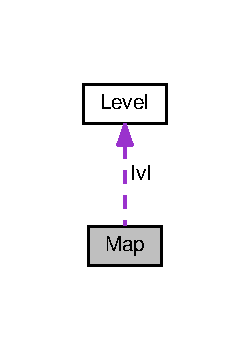
\includegraphics[width=120pt]{struct_map__coll__graph}
\end{center}
\end{figure}
\subsubsection*{Data Fields}
\begin{DoxyCompactItemize}
\item 
\hyperlink{struct_level}{Level} $\ast$ \hyperlink{struct_map_abca19b7de8e60347a507d1aeff95c764}{lvl}
\item 
int \hyperlink{struct_map_aa83bbdf2603e42824cd0bab44bf315c2}{x\-Scroll}
\item 
int \hyperlink{struct_map_ae50cb92a78d9e0a4f4bd718fc02bd294}{screen\-Width}
\item 
int \hyperlink{struct_map_a9ebc1dbd77788c4bfa27758a6725413f}{screen\-Height}
\end{DoxyCompactItemize}


\subsubsection{Detailed Description}
The map structure 

\subsubsection{Field Documentation}
\hypertarget{struct_map_abca19b7de8e60347a507d1aeff95c764}{\index{Map@{Map}!lvl@{lvl}}
\index{lvl@{lvl}!Map@{Map}}
\paragraph[{lvl}]{\setlength{\rightskip}{0pt plus 5cm}{\bf Level}$\ast$ lvl}}\label{struct_map_abca19b7de8e60347a507d1aeff95c764}
The level \hypertarget{struct_map_a9ebc1dbd77788c4bfa27758a6725413f}{\index{Map@{Map}!screen\-Height@{screen\-Height}}
\index{screen\-Height@{screen\-Height}!Map@{Map}}
\paragraph[{screen\-Height}]{\setlength{\rightskip}{0pt plus 5cm}int screen\-Height}}\label{struct_map_a9ebc1dbd77788c4bfa27758a6725413f}
The screen height \hypertarget{struct_map_ae50cb92a78d9e0a4f4bd718fc02bd294}{\index{Map@{Map}!screen\-Width@{screen\-Width}}
\index{screen\-Width@{screen\-Width}!Map@{Map}}
\paragraph[{screen\-Width}]{\setlength{\rightskip}{0pt plus 5cm}int screen\-Width}}\label{struct_map_ae50cb92a78d9e0a4f4bd718fc02bd294}
The Screen width \hypertarget{struct_map_aa83bbdf2603e42824cd0bab44bf315c2}{\index{Map@{Map}!x\-Scroll@{x\-Scroll}}
\index{x\-Scroll@{x\-Scroll}!Map@{Map}}
\paragraph[{x\-Scroll}]{\setlength{\rightskip}{0pt plus 5cm}int x\-Scroll}}\label{struct_map_aa83bbdf2603e42824cd0bab44bf315c2}
The xscroll 

The documentation for this struct was generated from the following file\-:\begin{DoxyCompactItemize}
\item 
\hyperlink{const_8h}{const.\-h}\end{DoxyCompactItemize}

\section{File Documentation}
\hypertarget{const_8h}{\section{const.\-h File Reference}
\label{const_8h}\index{const.\-h@{const.\-h}}
}


contient les constantes du programme  


This graph shows which files directly or indirectly include this file\-:\nopagebreak
\begin{figure}[H]
\begin{center}
\leavevmode
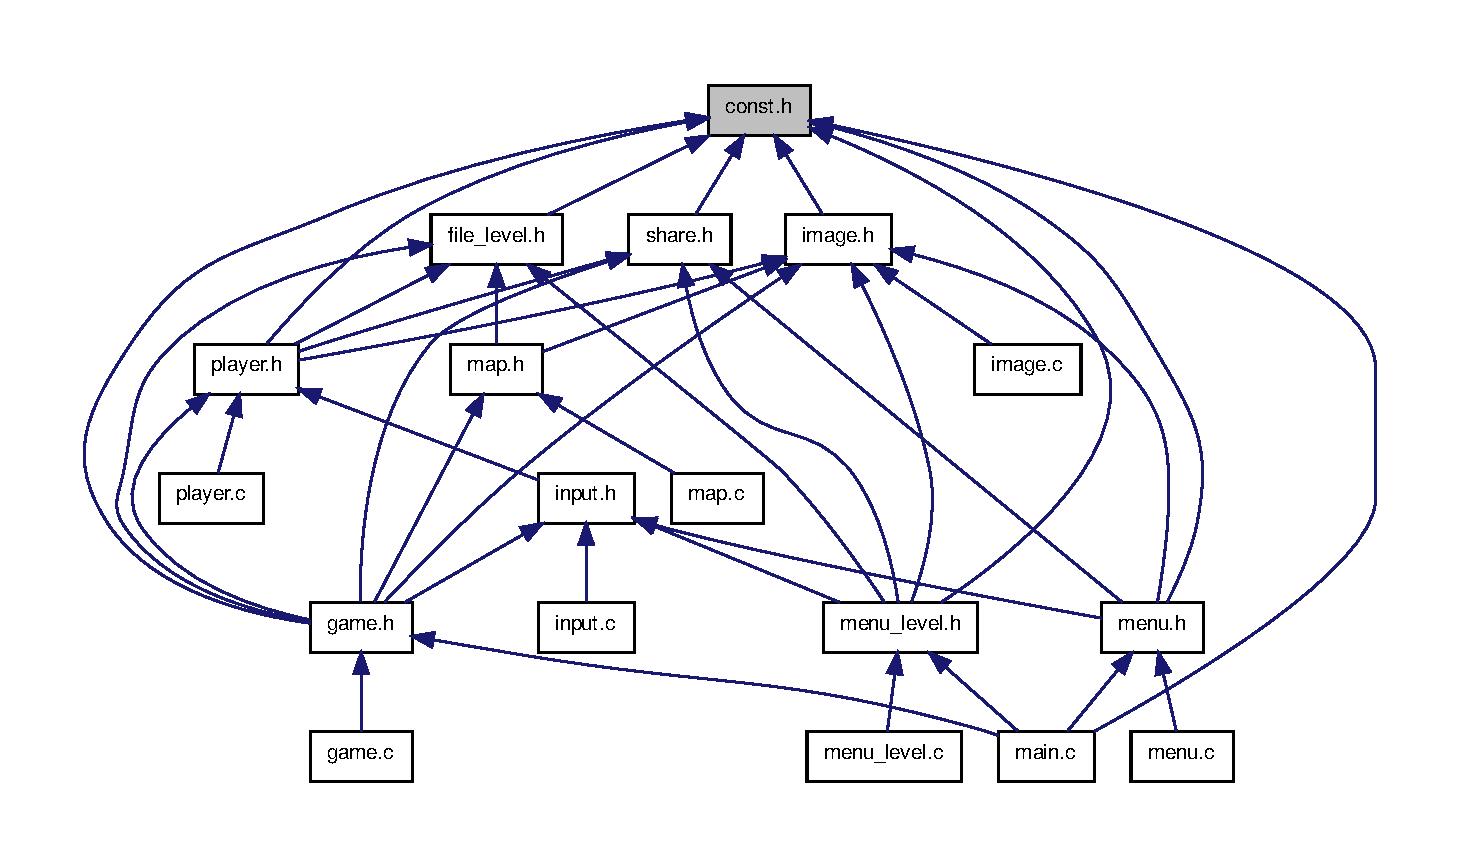
\includegraphics[width=350pt]{const_8h__dep__incl}
\end{center}
\end{figure}
\subsection*{Data Structures}
\begin{DoxyCompactItemize}
\item 
struct \hyperlink{struct_level}{Level}
\item 
struct \hyperlink{struct_map}{Map}
\end{DoxyCompactItemize}
\subsection*{Macros}
\begin{DoxyCompactItemize}
\item 
\hypertarget{const_8h_abad9ad5ae94fd56569e71c156349030b}{\#define {\bfseries T\-A\-I\-L\-L\-E\-\_\-\-B\-L\-O\-C}~16}\label{const_8h_abad9ad5ae94fd56569e71c156349030b}

\item 
\hypertarget{const_8h_a5b621c07985e98b04fc2d2195b85ad69}{\#define {\bfseries N\-B\-\_\-\-B\-L\-O\-C\-S\-\_\-\-L\-A\-R\-G\-E\-U\-R}~60}\label{const_8h_a5b621c07985e98b04fc2d2195b85ad69}

\item 
\hypertarget{const_8h_ad0de8de53b10369f89648fed34ce16c9}{\#define {\bfseries N\-B\-\_\-\-B\-L\-O\-C\-S\-\_\-\-H\-A\-U\-T\-E\-U\-R}~33}\label{const_8h_ad0de8de53b10369f89648fed34ce16c9}

\item 
\hypertarget{const_8h_a6068a247ff9ece1b0a9773c58144906c}{\#define {\bfseries L\-A\-R\-G\-E\-U\-R\-\_\-\-F\-E\-N\-E\-T\-R\-E}~T\-A\-I\-L\-L\-E\-\_\-\-B\-L\-O\-C $\ast$ N\-B\-\_\-\-B\-L\-O\-C\-S\-\_\-\-L\-A\-R\-G\-E\-U\-R}\label{const_8h_a6068a247ff9ece1b0a9773c58144906c}

\item 
\hypertarget{const_8h_afd1a1e285af564b849b17498e82e1a41}{\#define {\bfseries H\-A\-U\-T\-E\-U\-R\-\_\-\-F\-E\-N\-E\-T\-R\-E}~T\-A\-I\-L\-L\-E\-\_\-\-B\-L\-O\-C $\ast$ N\-B\-\_\-\-B\-L\-O\-C\-S\-\_\-\-H\-A\-U\-T\-E\-U\-R}\label{const_8h_afd1a1e285af564b849b17498e82e1a41}

\item 
\hypertarget{const_8h_ac92ca5ab87034a348decad7ee8d4bd1b}{\#define {\bfseries F\-P\-S}~60}\label{const_8h_ac92ca5ab87034a348decad7ee8d4bd1b}

\item 
\hypertarget{const_8h_a26141a4793db30295b597c3af901ddc8}{\#define {\bfseries T\-A\-I\-L\-L\-E\-\_\-\-M\-A\-X\-\_\-\-N\-O\-M\-\_\-\-F\-I\-C\-H\-I\-E\-R}~100}\label{const_8h_a26141a4793db30295b597c3af901ddc8}

\item 
\hypertarget{const_8h_a4295bab46a8fdcf8ff2106b2c32f15ad}{\#define {\bfseries T\-A\-I\-L\-L\-E\-\_\-\-S\-A\-U\-T}~17}\label{const_8h_a4295bab46a8fdcf8ff2106b2c32f15ad}

\item 
\hypertarget{const_8h_afe523953f60b9d8b73d97c8c673ef884}{\#define {\bfseries M\-A\-R\-G\-E\-\_\-\-S\-C\-R\-O\-L\-L\-I\-N\-G}~2}\label{const_8h_afe523953f60b9d8b73d97c8c673ef884}

\item 
\hypertarget{const_8h_a848d259eb2345aaa73fdfaeffb59afbd}{\#define {\bfseries P\-O\-U\-R\-C\-E\-N\-T\-A\-G\-E\-\_\-\-D\-E\-P\-L\-A\-C\-E\-M\-E\-N\-T}~0}\label{const_8h_a848d259eb2345aaa73fdfaeffb59afbd}

\item 
\hypertarget{const_8h_a95addb9496c5772d6e7bc43eabb16d8b}{\#define {\bfseries T\-I\-L\-E\-\_\-\-M\-A\-X}~8}\label{const_8h_a95addb9496c5772d6e7bc43eabb16d8b}

\end{DoxyCompactItemize}
\subsection*{Enumerations}
\begin{DoxyCompactItemize}
\item 
enum \{ {\bfseries V\-O\-I\-D} =0, 
{\bfseries G\-R\-A\-S\-S1} =1, 
{\bfseries G\-R\-O\-U\-N\-D1} =2, 
{\bfseries G\-R\-E\-Y\-\_\-\-W\-A\-L\-L} =3
 \}
\item 
enum \{ {\bfseries R\-I\-G\-H\-T}, 
{\bfseries L\-E\-F\-T}, 
{\bfseries U\-P}, 
{\bfseries D\-O\-W\-N}
 \}
\end{DoxyCompactItemize}


\subsection{Detailed Description}
contient les constantes du programme \begin{DoxyAuthor}{Author}
Xavier C\-O\-P\-O\-N\-E\-T 
\end{DoxyAuthor}
\begin{DoxyDate}{Date}
2014-\/02-\/27 
\end{DoxyDate}

\hypertarget{file_8c}{\section{file.\-c File Reference}
\label{file_8c}\index{file.\-c@{file.\-c}}
}


file access functions  


{\ttfamily \#include \char`\"{}file.\-h\char`\"{}}\\*
Include dependency graph for file.\-c\-:\nopagebreak
\begin{figure}[H]
\begin{center}
\leavevmode
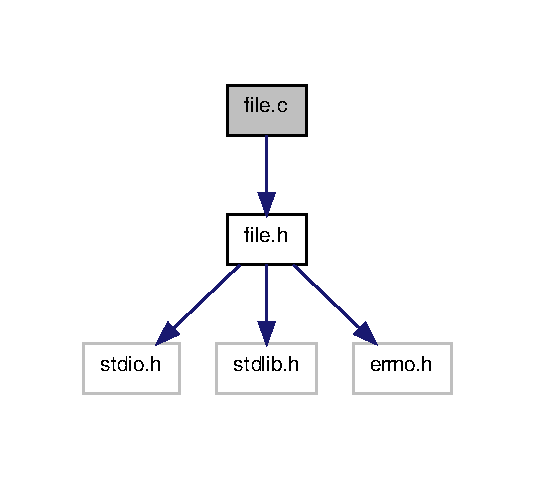
\includegraphics[width=256pt]{file_8c__incl}
\end{center}
\end{figure}
\subsection*{Functions}
\begin{DoxyCompactItemize}
\item 
F\-I\-L\-E $\ast$ \hyperlink{file_8c_ab763060cbdd57fdb704871d896fc492a}{open\-File} (char name\mbox{[}$\,$\mbox{]}, char mode\mbox{[}$\,$\mbox{]})
\item 
int \hyperlink{file_8c_adf55ac6bc5d81f94b54e4c8ea554f884}{close\-File} (F\-I\-L\-E $\ast$ptr\-\_\-file)
\end{DoxyCompactItemize}


\subsection{Detailed Description}
file access functions \begin{DoxyAuthor}{Author}
Remi B\-E\-R\-T\-H\-O 
\end{DoxyAuthor}
\begin{DoxyDate}{Date}
15/03/14 
\end{DoxyDate}


\subsection{Function Documentation}
\hypertarget{file_8c_adf55ac6bc5d81f94b54e4c8ea554f884}{\index{file.\-c@{file.\-c}!close\-File@{close\-File}}
\index{close\-File@{close\-File}!file.c@{file.\-c}}
\subsubsection[{close\-File}]{\setlength{\rightskip}{0pt plus 5cm}int close\-File (
\begin{DoxyParamCaption}
\item[{F\-I\-L\-E $\ast$}]{ptr\-\_\-file}
\end{DoxyParamCaption}
)}}\label{file_8c_adf55ac6bc5d81f94b54e4c8ea554f884}
close a file 
\begin{DoxyParams}[1]{Parameters}
\mbox{\tt in}  & {\em $\ast$ptr\-\_\-file} & the file to be closed \\
\hline
\end{DoxyParams}
\begin{DoxyReturn}{Returns}
int 0 if the file was succefuly closed, 1 if not 
\end{DoxyReturn}
\hypertarget{file_8c_ab763060cbdd57fdb704871d896fc492a}{\index{file.\-c@{file.\-c}!open\-File@{open\-File}}
\index{open\-File@{open\-File}!file.c@{file.\-c}}
\subsubsection[{open\-File}]{\setlength{\rightskip}{0pt plus 5cm}F\-I\-L\-E $\ast$ open\-File (
\begin{DoxyParamCaption}
\item[{char}]{name\mbox{[}$\,$\mbox{]}, }
\item[{char}]{mode\mbox{[}$\,$\mbox{]}}
\end{DoxyParamCaption}
)}}\label{file_8c_ab763060cbdd57fdb704871d896fc492a}
open a file 
\begin{DoxyParams}[1]{Parameters}
\mbox{\tt in}  & {\em name} & the file name/path \\
\hline
\mbox{\tt in}  & {\em mode} & the opening mode \\
\hline
\end{DoxyParams}
\begin{DoxyReturn}{Returns}
a pointer on the opened file, N\-U\-L\-L if error 
\end{DoxyReturn}

\hypertarget{file_8h}{\subsection{file.\-h File Reference}
\label{file_8h}\index{file.\-h@{file.\-h}}
}


\hyperlink{file_8c}{file.\-c} header  


{\ttfamily \#include $<$stdio.\-h$>$}\\*
{\ttfamily \#include $<$stdlib.\-h$>$}\\*
{\ttfamily \#include $<$errno.\-h$>$}\\*
\subsubsection*{Functions}
\begin{DoxyCompactItemize}
\item 
F\-I\-L\-E $\ast$ \hyperlink{file_8h_ae6218cf222b5ca17dce1ad7eb75346a9}{open\-File} (char nome\mbox{[}$\,$\mbox{]}, char mode\mbox{[}$\,$\mbox{]})
\item 
int \hyperlink{file_8h_a0fca34d72624f611d2cbeac47279bb1f}{close\-File} (F\-I\-L\-E $\ast$ptr\-\_\-fichier)
\end{DoxyCompactItemize}


\subsubsection{Detailed Description}
\hyperlink{file_8c}{file.\-c} header \begin{DoxyAuthor}{Author}
Remi B\-E\-R\-T\-H\-O, Glenn H\-E\-R\-R\-O\-U 
\end{DoxyAuthor}
\begin{DoxyDate}{Date}
2014-\/05-\/12 
\end{DoxyDate}


\subsubsection{Function Documentation}
\hypertarget{file_8h_a0fca34d72624f611d2cbeac47279bb1f}{\index{file.\-h@{file.\-h}!close\-File@{close\-File}}
\index{close\-File@{close\-File}!file.h@{file.\-h}}
\paragraph[{close\-File}]{\setlength{\rightskip}{0pt plus 5cm}int close\-File (
\begin{DoxyParamCaption}
\item[{F\-I\-L\-E $\ast$}]{ptr\-\_\-file}
\end{DoxyParamCaption}
)}}\label{file_8h_a0fca34d72624f611d2cbeac47279bb1f}
Close the given file 
\begin{DoxyParams}[1]{Parameters}
\mbox{\tt in}  & {\em $\ast$ptr\-\_\-file} & the file \\
\hline
\end{DoxyParams}
\begin{DoxyReturn}{Returns}
0 if the file has been succesfully closed, 1 otherwise 
\end{DoxyReturn}
\hypertarget{file_8h_ae6218cf222b5ca17dce1ad7eb75346a9}{\index{file.\-h@{file.\-h}!open\-File@{open\-File}}
\index{open\-File@{open\-File}!file.h@{file.\-h}}
\paragraph[{open\-File}]{\setlength{\rightskip}{0pt plus 5cm}F\-I\-L\-E$\ast$ open\-File (
\begin{DoxyParamCaption}
\item[{char}]{name\mbox{[}$\,$\mbox{]}, }
\item[{char}]{mode\mbox{[}$\,$\mbox{]}}
\end{DoxyParamCaption}
)}}\label{file_8h_ae6218cf222b5ca17dce1ad7eb75346a9}
Open a file which path is name with the given mode 
\begin{DoxyParams}[1]{Parameters}
\mbox{\tt in}  & {\em name\mbox{[}$\,$\mbox{]}} & name of the file \\
\hline
\mbox{\tt in}  & {\em mode\mbox{[}$\,$\mbox{]}} & the opening mode \\
\hline
\end{DoxyParams}
\begin{DoxyReturn}{Returns}
a pointer if the opening has been succesfull, N\-U\-L\-L otherwise 
\end{DoxyReturn}

\hypertarget{file__level_8c}{\subsection{file\-\_\-level.\-c File Reference}
\label{file__level_8c}\index{file\-\_\-level.\-c@{file\-\_\-level.\-c}}
}


map file gestion  


{\ttfamily \#include \char`\"{}file\-\_\-level.\-h\char`\"{}}\\*
\subsubsection*{Functions}
\begin{DoxyCompactItemize}
\item 
\hyperlink{struct_level}{Level} $\ast$ \hyperlink{file__level_8c_a8464887031ce16d797b564fc7a9e661f}{open\-Level} (char $\ast$file\-\_\-name, \hyperlink{structlist}{list} $\ast$l, \hyperlink{structplatform_set}{platform\-Set} $\ast$ps)
\item 
void \hyperlink{file__level_8c_a38020f30305d2344cdf39d06c7e8768e}{close\-Level} (\hyperlink{struct_level}{Level} $\ast$lvl)
\item 
\hyperlink{struct_level}{Level} $\ast$ \hyperlink{file__level_8c_a76e77e4f54cd176374bd70e25c1ffc07}{init\-Level} (\hyperlink{struct_level}{Level} $\ast$lvl)
\item 
char $\ast$$\ast$ \hyperlink{file__level_8c_a8f93e9edca6b3e54fa194e27bacf8f46}{read\-Level\-File} (char $\ast$file\-\_\-path, int $\ast$nb\-\_\-lvl)
\item 
void \hyperlink{file__level_8c_a3fafc12e3c322fc5a8166f7fb323bfe6}{close\-Level\-List} (char $\ast$$\ast$level\-\_\-names, int nb\-\_\-lvl)
\end{DoxyCompactItemize}


\subsubsection{Detailed Description}
map file gestion \begin{DoxyAuthor}{Author}
Remi B\-E\-R\-T\-H\-O 
\end{DoxyAuthor}
\begin{DoxyDate}{Date}
15/03/14 
\end{DoxyDate}
\begin{DoxyVersion}{Version}
1.\-0 
\end{DoxyVersion}


\subsubsection{Function Documentation}
\hypertarget{file__level_8c_a38020f30305d2344cdf39d06c7e8768e}{\index{file\-\_\-level.\-c@{file\-\_\-level.\-c}!close\-Level@{close\-Level}}
\index{close\-Level@{close\-Level}!file_level.c@{file\-\_\-level.\-c}}
\paragraph[{close\-Level}]{\setlength{\rightskip}{0pt plus 5cm}void close\-Level (
\begin{DoxyParamCaption}
\item[{{\bf Level} $\ast$}]{lvl}
\end{DoxyParamCaption}
)}}\label{file__level_8c_a38020f30305d2344cdf39d06c7e8768e}
close a level freeing its allocated memory 
\begin{DoxyParams}[1]{Parameters}
\mbox{\tt out}  & {\em lvl} & the level to be closed \\
\hline
\end{DoxyParams}
\hypertarget{file__level_8c_a3fafc12e3c322fc5a8166f7fb323bfe6}{\index{file\-\_\-level.\-c@{file\-\_\-level.\-c}!close\-Level\-List@{close\-Level\-List}}
\index{close\-Level\-List@{close\-Level\-List}!file_level.c@{file\-\_\-level.\-c}}
\paragraph[{close\-Level\-List}]{\setlength{\rightskip}{0pt plus 5cm}void close\-Level\-List (
\begin{DoxyParamCaption}
\item[{char $\ast$$\ast$}]{level\-\_\-names, }
\item[{int}]{nb\-\_\-lvl}
\end{DoxyParamCaption}
)}}\label{file__level_8c_a3fafc12e3c322fc5a8166f7fb323bfe6}
desallocate the level name list 
\begin{DoxyParams}[1]{Parameters}
\mbox{\tt in,out}  & {\em level\-\_\-names} & level name list \\
\hline
\mbox{\tt in}  & {\em nb\-\_\-lvl} & number of level \\
\hline
\end{DoxyParams}
\hypertarget{file__level_8c_a76e77e4f54cd176374bd70e25c1ffc07}{\index{file\-\_\-level.\-c@{file\-\_\-level.\-c}!init\-Level@{init\-Level}}
\index{init\-Level@{init\-Level}!file_level.c@{file\-\_\-level.\-c}}
\paragraph[{init\-Level}]{\setlength{\rightskip}{0pt plus 5cm}{\bf Level} $\ast$ init\-Level (
\begin{DoxyParamCaption}
\item[{{\bf Level} $\ast$}]{lvl}
\end{DoxyParamCaption}
)}}\label{file__level_8c_a76e77e4f54cd176374bd70e25c1ffc07}
Initialize a level assuming its width and height fields are already set 
\begin{DoxyParams}[1]{Parameters}
\mbox{\tt out}  & {\em lvl} & the level \\
\hline
\end{DoxyParams}
\begin{DoxyReturn}{Returns}
a pointer on the level structure 
\end{DoxyReturn}
\hypertarget{file__level_8c_a8464887031ce16d797b564fc7a9e661f}{\index{file\-\_\-level.\-c@{file\-\_\-level.\-c}!open\-Level@{open\-Level}}
\index{open\-Level@{open\-Level}!file_level.c@{file\-\_\-level.\-c}}
\paragraph[{open\-Level}]{\setlength{\rightskip}{0pt plus 5cm}{\bf Level} $\ast$ open\-Level (
\begin{DoxyParamCaption}
\item[{char $\ast$}]{file\-\_\-name, }
\item[{{\bf list} $\ast$}]{l, }
\item[{{\bf platform\-Set} $\ast$}]{ps}
\end{DoxyParamCaption}
)}}\label{file__level_8c_a8464887031ce16d797b564fc7a9e661f}
Open a map file and stock the map and the enemies 
\begin{DoxyParams}[1]{Parameters}
\mbox{\tt in}  & {\em file\-\_\-name} & the map file name \\
\hline
\mbox{\tt out}  & {\em l} & the enemy list to stock the enemies. \\
\hline
\mbox{\tt out}  & {\em ps} & the platform set for mobile platforms \\
\hline
\end{DoxyParams}
\begin{DoxyReturn}{Returns}
a pointer on the level structure 
\end{DoxyReturn}


Here is the call graph for this function\-:
\nopagebreak
\begin{figure}[H]
\begin{center}
\leavevmode
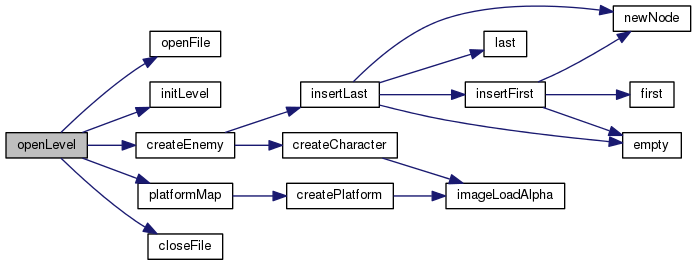
\includegraphics[width=350pt]{file__level_8c_a8464887031ce16d797b564fc7a9e661f_cgraph}
\end{center}
\end{figure}


\hypertarget{file__level_8c_a8f93e9edca6b3e54fa194e27bacf8f46}{\index{file\-\_\-level.\-c@{file\-\_\-level.\-c}!read\-Level\-File@{read\-Level\-File}}
\index{read\-Level\-File@{read\-Level\-File}!file_level.c@{file\-\_\-level.\-c}}
\paragraph[{read\-Level\-File}]{\setlength{\rightskip}{0pt plus 5cm}char $\ast$$\ast$ read\-Level\-File (
\begin{DoxyParamCaption}
\item[{char $\ast$}]{file\-\_\-path, }
\item[{int $\ast$}]{nb\-\_\-lvl}
\end{DoxyParamCaption}
)}}\label{file__level_8c_a8f93e9edca6b3e54fa194e27bacf8f46}
read a file level 
\begin{DoxyParams}[1]{Parameters}
\mbox{\tt out}  & {\em nb\-\_\-lvl} & number of level \\
\hline
\mbox{\tt out}  & {\em file\-\_\-path} & the file path \\
\hline
\end{DoxyParams}
\begin{DoxyReturn}{Returns}
pointer on the level list created 
\end{DoxyReturn}


Here is the call graph for this function\-:
\nopagebreak
\begin{figure}[H]
\begin{center}
\leavevmode
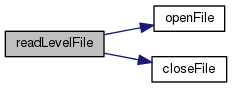
\includegraphics[width=246pt]{file__level_8c_a8f93e9edca6b3e54fa194e27bacf8f46_cgraph}
\end{center}
\end{figure}



\hypertarget{file__level_8h}{\subsection{file\-\_\-level.\-h File Reference}
\label{file__level_8h}\index{file\-\_\-level.\-h@{file\-\_\-level.\-h}}
}


\hyperlink{file__level_8c}{file\-\_\-level.\-c} header  


{\ttfamily \#include $<$stdio.\-h$>$}\\*
{\ttfamily \#include $<$stdlib.\-h$>$}\\*
{\ttfamily \#include $<$string.\-h$>$}\\*
{\ttfamily \#include \char`\"{}file.\-h\char`\"{}}\\*
{\ttfamily \#include \char`\"{}const.\-h\char`\"{}}\\*
{\ttfamily \#include \char`\"{}structures.\-h\char`\"{}}\\*
\subsubsection*{Macros}
\begin{DoxyCompactItemize}
\item 
\#define \hyperlink{file__level_8h_a6b20d41d6252e9871430c242cb1a56e7}{B\-U\-F\-F\-E\-R\-\_\-\-S\-I\-Z\-E}~2
\end{DoxyCompactItemize}
\subsubsection*{Functions}
\begin{DoxyCompactItemize}
\item 
\hyperlink{struct_level}{Level} $\ast$ \hyperlink{file__level_8h_a149f2e0878473ca6968717a39c119639}{open\-Level} (char $\ast$file\-\_\-name)
\item 
void \hyperlink{file__level_8h_a38020f30305d2344cdf39d06c7e8768e}{close\-Level} (\hyperlink{struct_level}{Level} $\ast$lvl)
\item 
\hyperlink{struct_level}{Level} $\ast$ \hyperlink{file__level_8h_a1749fb3f97d8b947c393f8eac9d29707}{init\-Level} (\hyperlink{struct_level}{Level} $\ast$lvl)
\item 
void \hyperlink{file__level_8h_aa22f94cc3689a4c98d553ff300c32bc9}{write\-Level} (char $\ast$file\-\_\-name, \hyperlink{struct_level}{Level} $\ast$lvl)
\item 
char $\ast$$\ast$ \hyperlink{file__level_8h_af646d7df8d540e24e2acc84fc3ea3ad3}{read\-Level\-File} (int $\ast$nb\-\_\-lvl)
\item 
void \hyperlink{file__level_8h_a3fafc12e3c322fc5a8166f7fb323bfe6}{close\-Level\-List} (char $\ast$$\ast$level\-\_\-names, int nb\-\_\-lvl)
\item 
\hyperlink{struct_level}{Level} $\ast$ \hyperlink{file__level_8h_a40c7ce420eb28ac24765fc244bd938ca}{adapt\-Size\-Level} (\hyperlink{struct_level}{Level} $\ast$lvl)
\item 
int \hyperlink{file__level_8h_abd4c02fab44779b57294a058c8486365}{search\-End\-Level} (\hyperlink{struct_level}{Level} $\ast$lvl)
\end{DoxyCompactItemize}


\subsubsection{Detailed Description}
\hyperlink{file__level_8c}{file\-\_\-level.\-c} header \begin{DoxyAuthor}{Author}
Remi B\-E\-R\-T\-H\-O, Glenn H\-E\-R\-R\-O\-U 
\end{DoxyAuthor}
\begin{DoxyDate}{Date}
2014-\/05-\/12 
\end{DoxyDate}
\begin{DoxyVersion}{Version}
2.\-0 
\end{DoxyVersion}


\subsubsection{Macro Definition Documentation}
\hypertarget{file__level_8h_a6b20d41d6252e9871430c242cb1a56e7}{\index{file\-\_\-level.\-h@{file\-\_\-level.\-h}!B\-U\-F\-F\-E\-R\-\_\-\-S\-I\-Z\-E@{B\-U\-F\-F\-E\-R\-\_\-\-S\-I\-Z\-E}}
\index{B\-U\-F\-F\-E\-R\-\_\-\-S\-I\-Z\-E@{B\-U\-F\-F\-E\-R\-\_\-\-S\-I\-Z\-E}!file_level.h@{file\-\_\-level.\-h}}
\paragraph[{B\-U\-F\-F\-E\-R\-\_\-\-S\-I\-Z\-E}]{\setlength{\rightskip}{0pt plus 5cm}\#define B\-U\-F\-F\-E\-R\-\_\-\-S\-I\-Z\-E~2}}\label{file__level_8h_a6b20d41d6252e9871430c242cb1a56e7}
The buffer size 

\subsubsection{Function Documentation}
\hypertarget{file__level_8h_a40c7ce420eb28ac24765fc244bd938ca}{\index{file\-\_\-level.\-h@{file\-\_\-level.\-h}!adapt\-Size\-Level@{adapt\-Size\-Level}}
\index{adapt\-Size\-Level@{adapt\-Size\-Level}!file_level.h@{file\-\_\-level.\-h}}
\paragraph[{adapt\-Size\-Level}]{\setlength{\rightskip}{0pt plus 5cm}{\bf Level}$\ast$ adapt\-Size\-Level (
\begin{DoxyParamCaption}
\item[{{\bf Level} $\ast$}]{lvl}
\end{DoxyParamCaption}
)}}\label{file__level_8h_a40c7ce420eb28ac24765fc244bd938ca}
Adapt the width of a level 
\begin{DoxyParams}[1]{Parameters}
\mbox{\tt in,out}  & {\em lvl} & the level to adapt \\
\hline
\end{DoxyParams}


Here is the call graph for this function\-:
\nopagebreak
\begin{figure}[H]
\begin{center}
\leavevmode
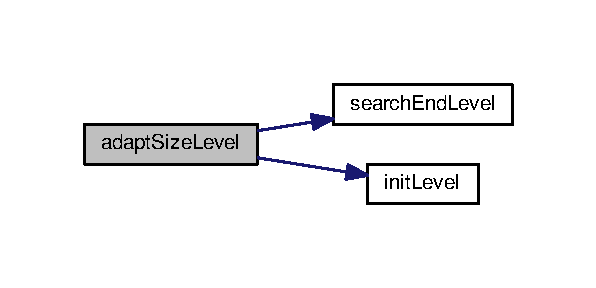
\includegraphics[width=286pt]{file__level_8h_a40c7ce420eb28ac24765fc244bd938ca_cgraph}
\end{center}
\end{figure}


\hypertarget{file__level_8h_a38020f30305d2344cdf39d06c7e8768e}{\index{file\-\_\-level.\-h@{file\-\_\-level.\-h}!close\-Level@{close\-Level}}
\index{close\-Level@{close\-Level}!file_level.h@{file\-\_\-level.\-h}}
\paragraph[{close\-Level}]{\setlength{\rightskip}{0pt plus 5cm}void close\-Level (
\begin{DoxyParamCaption}
\item[{{\bf Level} $\ast$}]{lvl}
\end{DoxyParamCaption}
)}}\label{file__level_8h_a38020f30305d2344cdf39d06c7e8768e}
Close a level by freeing its allocated memory 
\begin{DoxyParams}[1]{Parameters}
\mbox{\tt out}  & {\em lvl} & The level \\
\hline
\end{DoxyParams}
\hypertarget{file__level_8h_a3fafc12e3c322fc5a8166f7fb323bfe6}{\index{file\-\_\-level.\-h@{file\-\_\-level.\-h}!close\-Level\-List@{close\-Level\-List}}
\index{close\-Level\-List@{close\-Level\-List}!file_level.h@{file\-\_\-level.\-h}}
\paragraph[{close\-Level\-List}]{\setlength{\rightskip}{0pt plus 5cm}void close\-Level\-List (
\begin{DoxyParamCaption}
\item[{char $\ast$$\ast$}]{level\-\_\-names, }
\item[{int}]{nb\-\_\-lvl}
\end{DoxyParamCaption}
)}}\label{file__level_8h_a3fafc12e3c322fc5a8166f7fb323bfe6}
Free the array containing the list of the levels 
\begin{DoxyParams}[1]{Parameters}
\mbox{\tt in,out}  & {\em level\-\_\-names} & the list of existing levels \\
\hline
\mbox{\tt in}  & {\em nb\-\_\-lvl} & the number of existing levels \\
\hline
\end{DoxyParams}
\hypertarget{file__level_8h_a1749fb3f97d8b947c393f8eac9d29707}{\index{file\-\_\-level.\-h@{file\-\_\-level.\-h}!init\-Level@{init\-Level}}
\index{init\-Level@{init\-Level}!file_level.h@{file\-\_\-level.\-h}}
\paragraph[{init\-Level}]{\setlength{\rightskip}{0pt plus 5cm}{\bf Level}$\ast$ init\-Level (
\begin{DoxyParamCaption}
\item[{{\bf Level} $\ast$}]{lvl}
\end{DoxyParamCaption}
)}}\label{file__level_8h_a1749fb3f97d8b947c393f8eac9d29707}
Initialize a level. The width and the Height of the level must be stored in the level before calling this function. 
\begin{DoxyParams}[1]{Parameters}
\mbox{\tt out}  & {\em lvl} & The level \\
\hline
\end{DoxyParams}
\begin{DoxyReturn}{Returns}
a pointer on the level initialized 
\end{DoxyReturn}
\hypertarget{file__level_8h_a149f2e0878473ca6968717a39c119639}{\index{file\-\_\-level.\-h@{file\-\_\-level.\-h}!open\-Level@{open\-Level}}
\index{open\-Level@{open\-Level}!file_level.h@{file\-\_\-level.\-h}}
\paragraph[{open\-Level}]{\setlength{\rightskip}{0pt plus 5cm}{\bf Level}$\ast$ open\-Level (
\begin{DoxyParamCaption}
\item[{char $\ast$}]{file\-\_\-name}
\end{DoxyParamCaption}
)}}\label{file__level_8h_a149f2e0878473ca6968717a39c119639}
Open a level file and store the level corresponding to the file 
\begin{DoxyParams}[1]{Parameters}
\mbox{\tt in}  & {\em file\-\_\-name} & the name of the level file \\
\hline
\end{DoxyParams}
\begin{DoxyReturn}{Returns}
a pointer to the level created 
\end{DoxyReturn}


Here is the call graph for this function\-:
\nopagebreak
\begin{figure}[H]
\begin{center}
\leavevmode
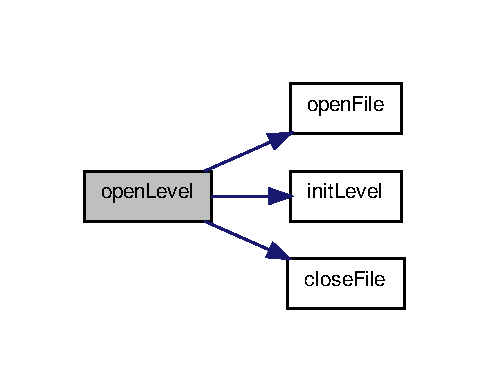
\includegraphics[width=234pt]{file__level_8h_a149f2e0878473ca6968717a39c119639_cgraph}
\end{center}
\end{figure}


\hypertarget{file__level_8h_af646d7df8d540e24e2acc84fc3ea3ad3}{\index{file\-\_\-level.\-h@{file\-\_\-level.\-h}!read\-Level\-File@{read\-Level\-File}}
\index{read\-Level\-File@{read\-Level\-File}!file_level.h@{file\-\_\-level.\-h}}
\paragraph[{read\-Level\-File}]{\setlength{\rightskip}{0pt plus 5cm}char$\ast$$\ast$ read\-Level\-File (
\begin{DoxyParamCaption}
\item[{int $\ast$}]{nb\-\_\-lvl}
\end{DoxyParamCaption}
)}}\label{file__level_8h_af646d7df8d540e24e2acc84fc3ea3ad3}
Read the file including the list of existing levels 
\begin{DoxyParams}[1]{Parameters}
\mbox{\tt out}  & {\em nb\-\_\-lvl} & the number of level in the file \\
\hline
\end{DoxyParams}
\begin{DoxyReturn}{Returns}
a pointer to an array of strings containing the list of the levels 
\end{DoxyReturn}


Here is the call graph for this function\-:
\nopagebreak
\begin{figure}[H]
\begin{center}
\leavevmode
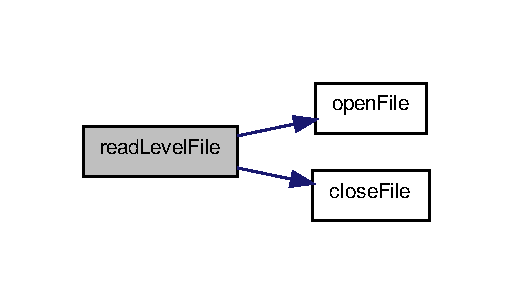
\includegraphics[width=246pt]{file__level_8h_af646d7df8d540e24e2acc84fc3ea3ad3_cgraph}
\end{center}
\end{figure}


\hypertarget{file__level_8h_abd4c02fab44779b57294a058c8486365}{\index{file\-\_\-level.\-h@{file\-\_\-level.\-h}!search\-End\-Level@{search\-End\-Level}}
\index{search\-End\-Level@{search\-End\-Level}!file_level.h@{file\-\_\-level.\-h}}
\paragraph[{search\-End\-Level}]{\setlength{\rightskip}{0pt plus 5cm}int search\-End\-Level (
\begin{DoxyParamCaption}
\item[{{\bf Level} $\ast$}]{lvl}
\end{DoxyParamCaption}
)}}\label{file__level_8h_abd4c02fab44779b57294a058c8486365}
Search the end of a level 
\begin{DoxyParams}[1]{Parameters}
\mbox{\tt in,out}  & {\em lvl} & the level \\
\hline
\end{DoxyParams}
\hypertarget{file__level_8h_aa22f94cc3689a4c98d553ff300c32bc9}{\index{file\-\_\-level.\-h@{file\-\_\-level.\-h}!write\-Level@{write\-Level}}
\index{write\-Level@{write\-Level}!file_level.h@{file\-\_\-level.\-h}}
\paragraph[{write\-Level}]{\setlength{\rightskip}{0pt plus 5cm}void write\-Level (
\begin{DoxyParamCaption}
\item[{char $\ast$}]{file\-\_\-name, }
\item[{{\bf Level} $\ast$}]{lvl}
\end{DoxyParamCaption}
)}}\label{file__level_8h_aa22f94cc3689a4c98d553ff300c32bc9}
Write the given level in the given file 
\begin{DoxyParams}[1]{Parameters}
\mbox{\tt in}  & {\em lvl} & the file \\
\hline
\mbox{\tt in}  & {\em file\-\_\-name} & the name of the file \\
\hline
\end{DoxyParams}


Here is the call graph for this function\-:
\nopagebreak
\begin{figure}[H]
\begin{center}
\leavevmode
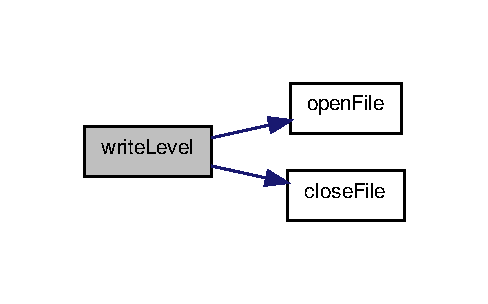
\includegraphics[width=350pt]{file__level_8h_aa22f94cc3689a4c98d553ff300c32bc9_cgraph}
\end{center}
\end{figure}



\hypertarget{game_8c}{\subsection{game.\-c File Reference}
\label{game_8c}\index{game.\-c@{game.\-c}}
}


Contain the main functions of the game.  


{\ttfamily \#include \char`\"{}game.\-h\char`\"{}}\\*
\subsubsection*{Functions}
\begin{DoxyCompactItemize}
\item 
void \hyperlink{game_8c_a3be984c6f3d228041d098485fe01f98c}{play} (S\-D\-L\-\_\-\-Surface $\ast$screen, char $\ast$level\-\_\-name, S\-D\-L\-Key $\ast$kc)
\item 
void \hyperlink{game_8c_aef36043913d82479cc03e51d01a320a1}{print\-Confirmation} (S\-D\-L\-\_\-\-Surface $\ast$screen, \hyperlink{struct_input}{Input} $\ast$in, int $\ast$go)
\end{DoxyCompactItemize}


\subsubsection{Detailed Description}
Contain the main functions of the game. \begin{DoxyAuthor}{Author}
Xavier C\-O\-P\-O\-N\-E\-T, Glenn H\-E\-R\-R\-O\-U 
\end{DoxyAuthor}
\begin{DoxyDate}{Date}
2014-\/05-\/15 
\end{DoxyDate}


\subsubsection{Function Documentation}
\hypertarget{game_8c_a3be984c6f3d228041d098485fe01f98c}{\index{game.\-c@{game.\-c}!play@{play}}
\index{play@{play}!game.c@{game.\-c}}
\paragraph[{play}]{\setlength{\rightskip}{0pt plus 5cm}void play (
\begin{DoxyParamCaption}
\item[{S\-D\-L\-\_\-\-Surface $\ast$}]{screen, }
\item[{char $\ast$}]{level\-\_\-name, }
\item[{S\-D\-L\-Key $\ast$}]{kc}
\end{DoxyParamCaption}
)}}\label{game_8c_a3be984c6f3d228041d098485fe01f98c}
Include the main loop of the game 
\begin{DoxyParams}[1]{Parameters}
\mbox{\tt in,out}  & {\em screen} & The screen of the game \\
\hline
\mbox{\tt in}  & {\em level\-\_\-name} & The name of the level \\
\hline
\mbox{\tt in}  & {\em kc} & The keyboard configuration \\
\hline
\end{DoxyParams}


Here is the call graph for this function\-:
\nopagebreak
\begin{figure}[H]
\begin{center}
\leavevmode
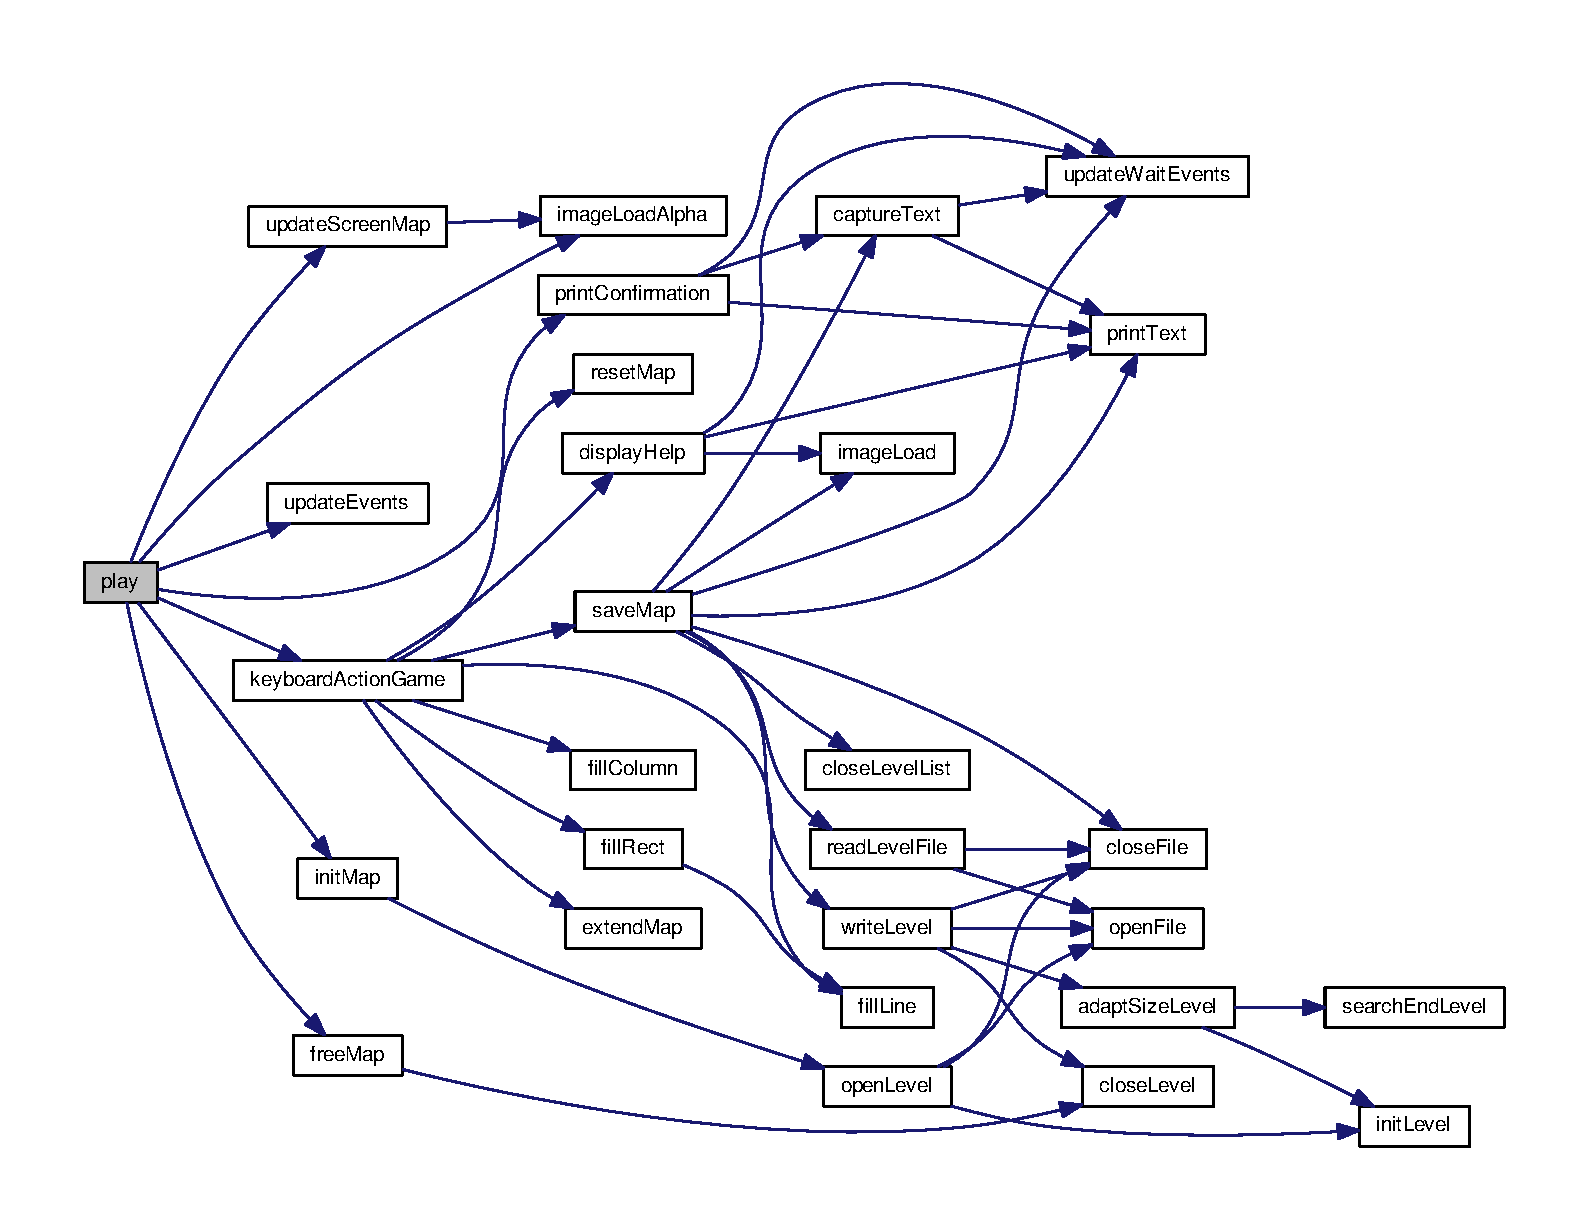
\includegraphics[width=350pt]{game_8c_a3be984c6f3d228041d098485fe01f98c_cgraph}
\end{center}
\end{figure}


\hypertarget{game_8c_aef36043913d82479cc03e51d01a320a1}{\index{game.\-c@{game.\-c}!print\-Confirmation@{print\-Confirmation}}
\index{print\-Confirmation@{print\-Confirmation}!game.c@{game.\-c}}
\paragraph[{print\-Confirmation}]{\setlength{\rightskip}{0pt plus 5cm}void print\-Confirmation (
\begin{DoxyParamCaption}
\item[{S\-D\-L\-\_\-\-Surface $\ast$}]{screen, }
\item[{{\bf Input} $\ast$}]{in, }
\item[{int $\ast$}]{go}
\end{DoxyParamCaption}
)}}\label{game_8c_aef36043913d82479cc03e51d01a320a1}
Display the confirmation screen, before leaving the edition of a level 
\begin{DoxyParams}[1]{Parameters}
\mbox{\tt out}  & {\em screen} & The screen of the game \\
\hline
\mbox{\tt in}  & {\em in} & The input structure \\
\hline
\mbox{\tt out}  & {\em go} & The main loop activation \\
\hline
\end{DoxyParams}


Here is the call graph for this function\-:
\nopagebreak
\begin{figure}[H]
\begin{center}
\leavevmode
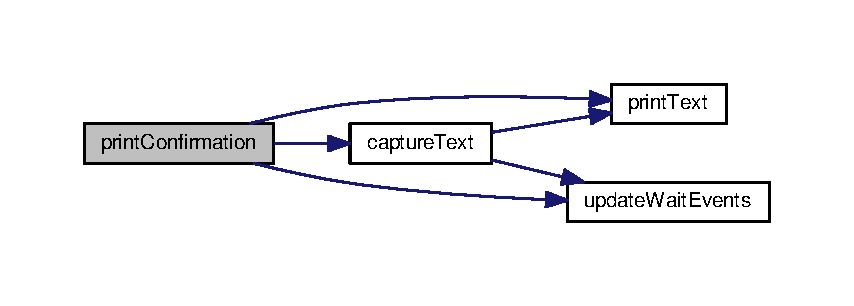
\includegraphics[width=350pt]{game_8c_aef36043913d82479cc03e51d01a320a1_cgraph}
\end{center}
\end{figure}



\hypertarget{game_8h}{\section{game.\-h File Reference}
\label{game_8h}\index{game.\-h@{game.\-h}}
}


Header of \hyperlink{game_8c}{game.\-c}.  


{\ttfamily \#include \char`\"{}const.\-h\char`\"{}}\\*
{\ttfamily \#include \char`\"{}file\-\_\-level.\-h\char`\"{}}\\*
{\ttfamily \#include \char`\"{}input.\-h\char`\"{}}\\*
{\ttfamily \#include \char`\"{}map.\-h\char`\"{}}\\*
Include dependency graph for game.\-h\-:\nopagebreak
\begin{figure}[H]
\begin{center}
\leavevmode
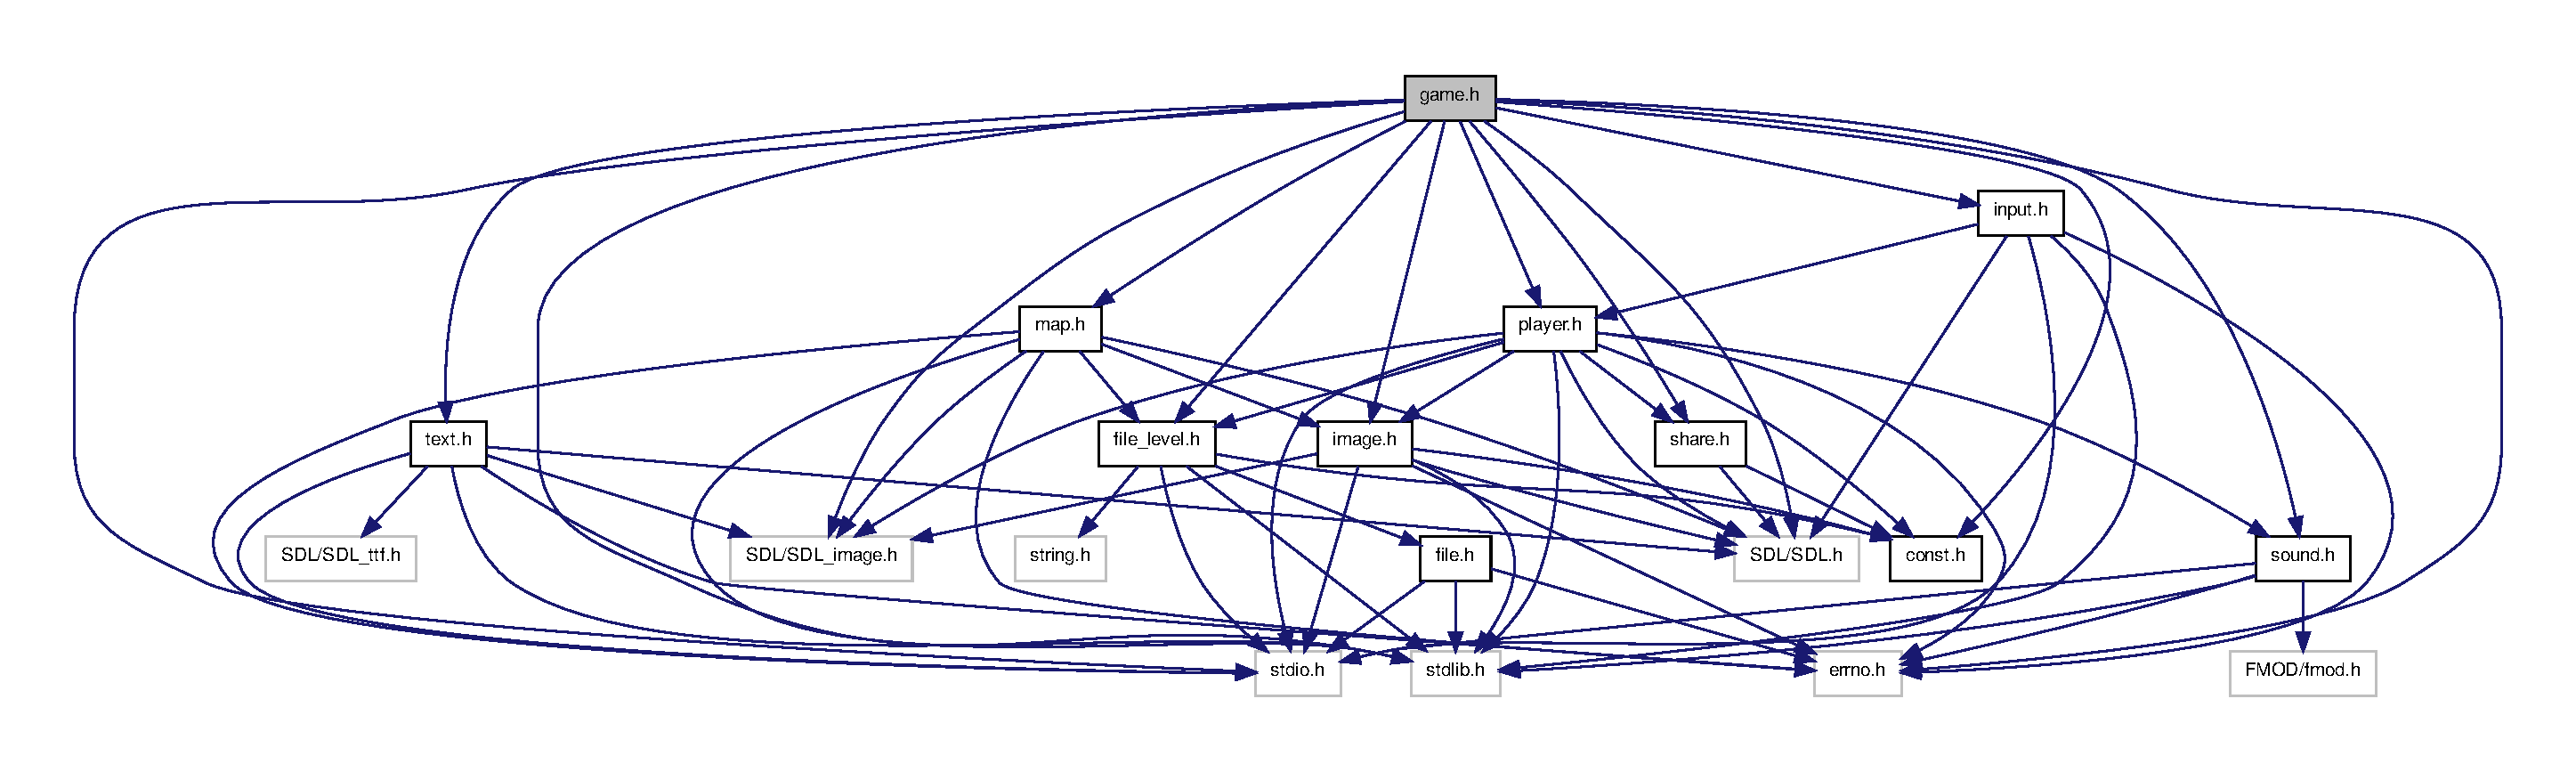
\includegraphics[width=350pt]{game_8h__incl}
\end{center}
\end{figure}
This graph shows which files directly or indirectly include this file\-:
\nopagebreak
\begin{figure}[H]
\begin{center}
\leavevmode
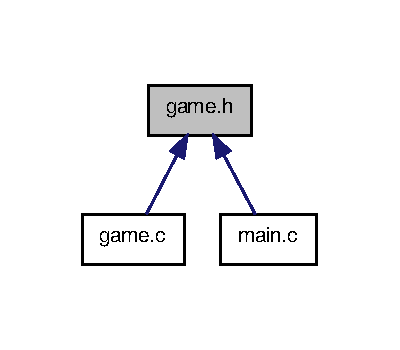
\includegraphics[width=254pt]{game_8h__dep__incl}
\end{center}
\end{figure}
\subsection*{Functions}
\begin{DoxyCompactItemize}
\item 
void \hyperlink{game_8h_ae342e4b762af0d52f4ee914643441426}{play} (S\-D\-L\-\_\-\-Surface $\ast$screen, char $\ast$level\-\_\-name)
\end{DoxyCompactItemize}


\subsection{Detailed Description}
Header of \hyperlink{game_8c}{game.\-c}. \begin{DoxyAuthor}{Author}
Xavier C\-O\-P\-O\-N\-E\-T, Glenn H\-E\-R\-R\-O\-U 
\end{DoxyAuthor}
\begin{DoxyDate}{Date}
2014-\/03-\/18 
\end{DoxyDate}


\subsection{Function Documentation}
\hypertarget{game_8h_ae342e4b762af0d52f4ee914643441426}{\index{game.\-h@{game.\-h}!play@{play}}
\index{play@{play}!game.h@{game.\-h}}
\subsubsection[{play}]{\setlength{\rightskip}{0pt plus 5cm}void play (
\begin{DoxyParamCaption}
\item[{S\-D\-L\-\_\-\-Surface $\ast$}]{screen, }
\item[{char $\ast$}]{level\-\_\-name}
\end{DoxyParamCaption}
)}}\label{game_8h_ae342e4b762af0d52f4ee914643441426}
Contains the infinite loop of the game, call the main functions 
\begin{DoxyParams}[1]{Parameters}
\mbox{\tt in,out}  & {\em screen} & Game screen \\
\hline
\mbox{\tt in}  & {\em level\-\_\-name} & \hyperlink{struct_level}{Level} name \\
\hline
\end{DoxyParams}


Here is the call graph for this function\-:
\nopagebreak
\begin{figure}[H]
\begin{center}
\leavevmode
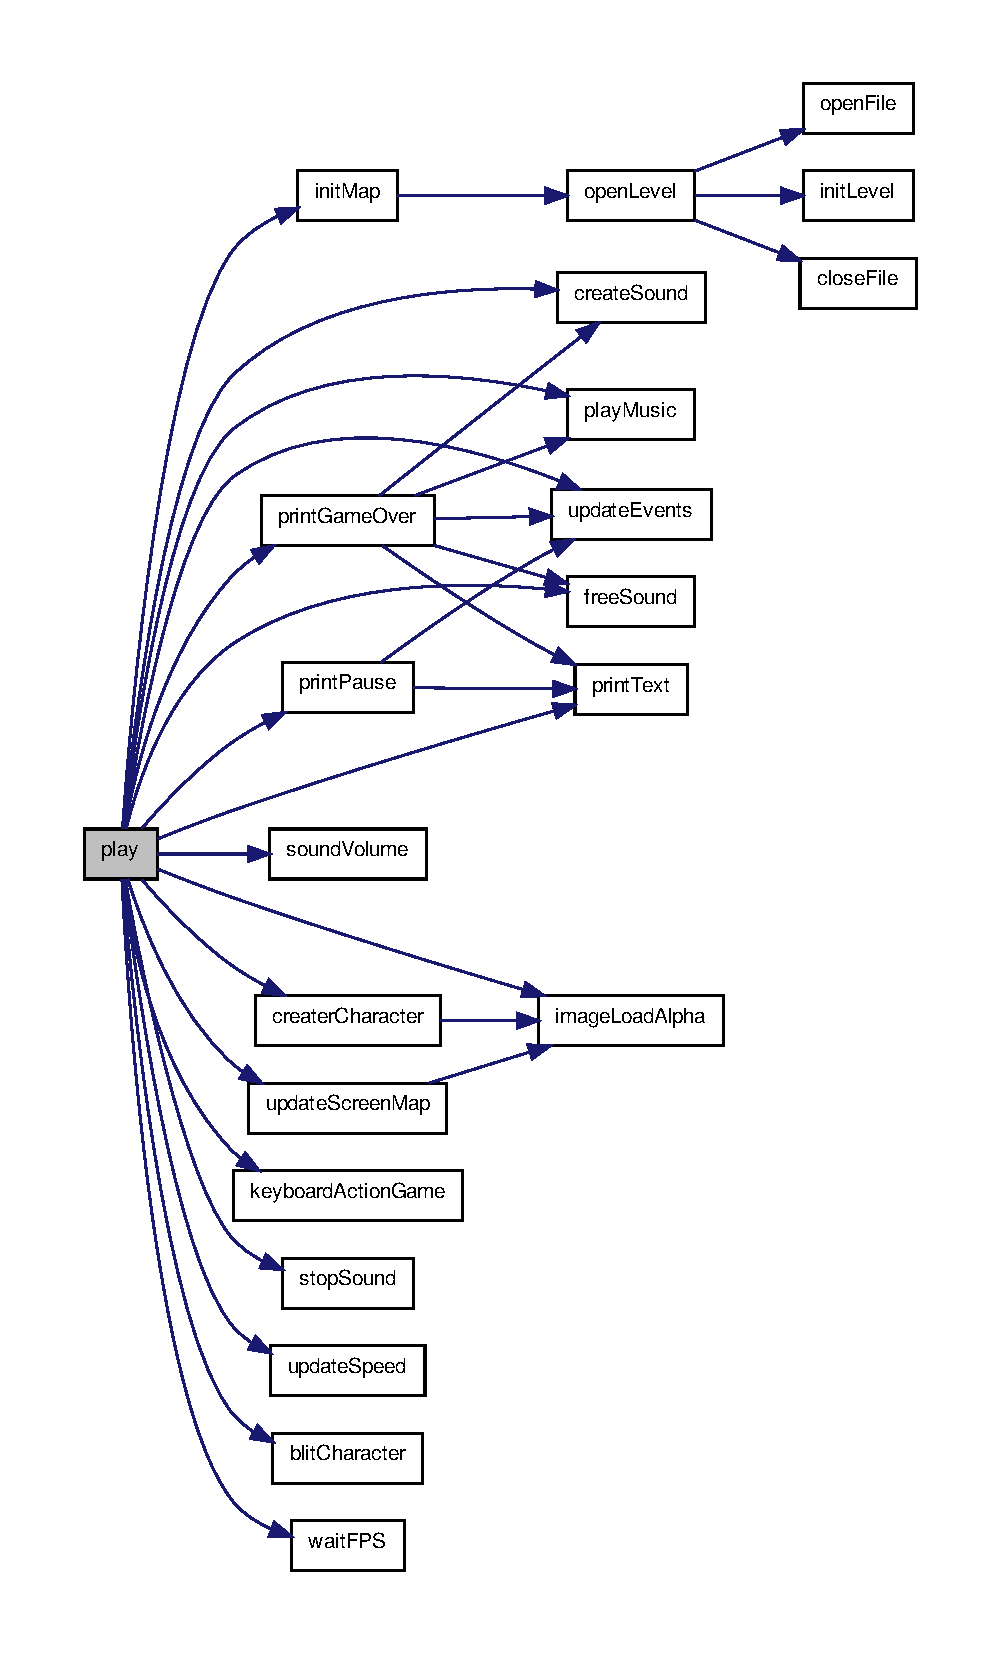
\includegraphics[width=306pt]{game_8h_ae342e4b762af0d52f4ee914643441426_cgraph}
\end{center}
\end{figure}



\hypertarget{image_8c}{\subsection{image.\-c File Reference}
\label{image_8c}\index{image.\-c@{image.\-c}}
}


Contain the functions managing the images.  


{\ttfamily \#include \char`\"{}image.\-h\char`\"{}}\\*
\subsubsection*{Functions}
\begin{DoxyCompactItemize}
\item 
S\-D\-L\-\_\-\-Surface $\ast$ \hyperlink{image_8c_a9862daea48ad8bfd1d3a0c401a9f5210}{image\-Load} (char $\ast$file\-\_\-name)
\item 
S\-D\-L\-\_\-\-Surface $\ast$ \hyperlink{image_8c_a569b068180b77bf2d44cf580322c68ad}{image\-Load\-Alpha} (char $\ast$file\-\_\-name)
\item 
void \hyperlink{image_8c_a3917cdd2e4b298f247aedfdf76268c75}{blit\-Color} (Uint32 red, Uint32 green, Uint32 blue, int alpha, S\-D\-L\-\_\-\-Surface $\ast$screen)
\end{DoxyCompactItemize}


\subsubsection{Detailed Description}
Contain the functions managing the images. \begin{DoxyAuthor}{Author}
Rémi B\-E\-R\-T\-H\-O 
\end{DoxyAuthor}
\begin{DoxyDate}{Date}
2014-\/02-\/27 
\end{DoxyDate}


\subsubsection{Function Documentation}
\hypertarget{image_8c_a3917cdd2e4b298f247aedfdf76268c75}{\index{image.\-c@{image.\-c}!blit\-Color@{blit\-Color}}
\index{blit\-Color@{blit\-Color}!image.c@{image.\-c}}
\paragraph[{blit\-Color}]{\setlength{\rightskip}{0pt plus 5cm}void blit\-Color (
\begin{DoxyParamCaption}
\item[{Uint32}]{red, }
\item[{Uint32}]{green, }
\item[{Uint32}]{blue, }
\item[{int}]{alpha, }
\item[{S\-D\-L\-\_\-\-Surface $\ast$}]{screen}
\end{DoxyParamCaption}
)}}\label{image_8c_a3917cdd2e4b298f247aedfdf76268c75}
Blit a color on the screen 
\begin{DoxyParams}[1]{Parameters}
\mbox{\tt in}  & {\em red} & the red of the color \\
\hline
\mbox{\tt in}  & {\em green} & the green of the color \\
\hline
\mbox{\tt in}  & {\em blue} & the blue of the color \\
\hline
\mbox{\tt in}  & {\em alpha} & the transparency of the image file \\
\hline
\mbox{\tt in}  & {\em screen} & the screen \\
\hline
\end{DoxyParams}
\hypertarget{image_8c_a9862daea48ad8bfd1d3a0c401a9f5210}{\index{image.\-c@{image.\-c}!image\-Load@{image\-Load}}
\index{image\-Load@{image\-Load}!image.c@{image.\-c}}
\paragraph[{image\-Load}]{\setlength{\rightskip}{0pt plus 5cm}S\-D\-L\-\_\-\-Surface $\ast$ image\-Load (
\begin{DoxyParamCaption}
\item[{char $\ast$}]{file\-\_\-name}
\end{DoxyParamCaption}
)}}\label{image_8c_a9862daea48ad8bfd1d3a0c401a9f5210}
Load an image 
\begin{DoxyParams}[1]{Parameters}
\mbox{\tt in}  & {\em file\-\_\-name} & the name of the image file \\
\hline
\end{DoxyParams}
\begin{DoxyReturn}{Returns}
a pointer on the S\-D\-L\-\_\-\-Surface created 
\end{DoxyReturn}
\hypertarget{image_8c_a569b068180b77bf2d44cf580322c68ad}{\index{image.\-c@{image.\-c}!image\-Load\-Alpha@{image\-Load\-Alpha}}
\index{image\-Load\-Alpha@{image\-Load\-Alpha}!image.c@{image.\-c}}
\paragraph[{image\-Load\-Alpha}]{\setlength{\rightskip}{0pt plus 5cm}S\-D\-L\-\_\-\-Surface $\ast$ image\-Load\-Alpha (
\begin{DoxyParamCaption}
\item[{char $\ast$}]{file\-\_\-name}
\end{DoxyParamCaption}
)}}\label{image_8c_a569b068180b77bf2d44cf580322c68ad}
Load an image with alpha management 
\begin{DoxyParams}[1]{Parameters}
\mbox{\tt in}  & {\em file\-\_\-name} & the name of the image file \\
\hline
\end{DoxyParams}
\begin{DoxyReturn}{Returns}
a pointer on the S\-D\-L\-\_\-\-Surface created 
\end{DoxyReturn}

\hypertarget{image_8h}{\subsection{image.\-h File Reference}
\label{image_8h}\index{image.\-h@{image.\-h}}
}


contient les fonction liées aux images  


{\ttfamily \#include $<$stdlib.\-h$>$}\\*
{\ttfamily \#include $<$stdio.\-h$>$}\\*
{\ttfamily \#include $<$errno.\-h$>$}\\*
{\ttfamily \#include $<$S\-D\-L/\-S\-D\-L.\-h$>$}\\*
{\ttfamily \#include $<$S\-D\-L/\-S\-D\-L\-\_\-image.\-h$>$}\\*
{\ttfamily \#include \char`\"{}const.\-h\char`\"{}}\\*
\subsubsection*{Functions}
\begin{DoxyCompactItemize}
\item 
S\-D\-L\-\_\-\-Surface $\ast$ \hyperlink{image_8h_aa53e98f2ff3d527d25b36023ea7f9d56}{image\-Load} (char $\ast$file\-\_\-name)
\item 
S\-D\-L\-\_\-\-Surface $\ast$ \hyperlink{image_8h_a469cf40e18cf579993e349b4393a2876}{image\-Load\-Alpha} (char $\ast$file\-\_\-name)
\item 
void \hyperlink{image_8h_a3917cdd2e4b298f247aedfdf76268c75}{blit\-Color} (Uint32 red, Uint32 green, Uint32 blue, int alpha, S\-D\-L\-\_\-\-Surface $\ast$screen)
\end{DoxyCompactItemize}


\subsubsection{Detailed Description}
contient les fonction liées aux images \begin{DoxyAuthor}{Author}
Rémi B\-E\-R\-T\-H\-O 
\end{DoxyAuthor}
\begin{DoxyDate}{Date}
2014-\/02-\/27 
\end{DoxyDate}


\subsubsection{Function Documentation}
\hypertarget{image_8h_a3917cdd2e4b298f247aedfdf76268c75}{\index{image.\-h@{image.\-h}!blit\-Color@{blit\-Color}}
\index{blit\-Color@{blit\-Color}!image.h@{image.\-h}}
\paragraph[{blit\-Color}]{\setlength{\rightskip}{0pt plus 5cm}void blit\-Color (
\begin{DoxyParamCaption}
\item[{Uint32}]{red, }
\item[{Uint32}]{green, }
\item[{Uint32}]{blue, }
\item[{int}]{alpha, }
\item[{S\-D\-L\-\_\-\-Surface $\ast$}]{screen}
\end{DoxyParamCaption}
)}}\label{image_8h_a3917cdd2e4b298f247aedfdf76268c75}
Blit a color on the screen 
\begin{DoxyParams}[1]{Parameters}
\mbox{\tt in}  & {\em red} & the red of the color \\
\hline
\mbox{\tt in}  & {\em green} & the green of the color \\
\hline
\mbox{\tt in}  & {\em blue} & the blue of the color \\
\hline
\mbox{\tt in}  & {\em alpha} & the transparency of the image file \\
\hline
\mbox{\tt in}  & {\em screen} & the screen \\
\hline
\end{DoxyParams}
\hypertarget{image_8h_aa53e98f2ff3d527d25b36023ea7f9d56}{\index{image.\-h@{image.\-h}!image\-Load@{image\-Load}}
\index{image\-Load@{image\-Load}!image.h@{image.\-h}}
\paragraph[{image\-Load}]{\setlength{\rightskip}{0pt plus 5cm}S\-D\-L\-\_\-\-Surface$\ast$ image\-Load (
\begin{DoxyParamCaption}
\item[{char $\ast$}]{file\-\_\-name}
\end{DoxyParamCaption}
)}}\label{image_8h_aa53e98f2ff3d527d25b36023ea7f9d56}
Load an image 
\begin{DoxyParams}[1]{Parameters}
\mbox{\tt in}  & {\em file\-\_\-name} & the name of the image file \\
\hline
\end{DoxyParams}
\begin{DoxyReturn}{Returns}
a pointer on the S\-D\-L\-\_\-\-Surface created 
\end{DoxyReturn}
\hypertarget{image_8h_a469cf40e18cf579993e349b4393a2876}{\index{image.\-h@{image.\-h}!image\-Load\-Alpha@{image\-Load\-Alpha}}
\index{image\-Load\-Alpha@{image\-Load\-Alpha}!image.h@{image.\-h}}
\paragraph[{image\-Load\-Alpha}]{\setlength{\rightskip}{0pt plus 5cm}S\-D\-L\-\_\-\-Surface$\ast$ image\-Load\-Alpha (
\begin{DoxyParamCaption}
\item[{char $\ast$}]{file\-\_\-name}
\end{DoxyParamCaption}
)}}\label{image_8h_a469cf40e18cf579993e349b4393a2876}
Load an image with alpha management 
\begin{DoxyParams}[1]{Parameters}
\mbox{\tt in}  & {\em file\-\_\-name} & the name of the image file \\
\hline
\end{DoxyParams}
\begin{DoxyReturn}{Returns}
a pointer on the S\-D\-L\-\_\-\-Surface created 
\end{DoxyReturn}

\hypertarget{input_8c}{\subsection{input.\-c File Reference}
\label{input_8c}\index{input.\-c@{input.\-c}}
}
{\ttfamily \#include \char`\"{}input.\-h\char`\"{}}\\*
\subsubsection*{Functions}
\begin{DoxyCompactItemize}
\item 
void \hyperlink{input_8c_a907831170dedec3a0af4e4b1e178b854}{update\-Events} (\hyperlink{struct_input}{Input} $\ast$in)
\item 
void \hyperlink{input_8c_a0f2aa7e2cd7674e43532893e4f2802e8}{keyboard\-Action\-Game} (S\-D\-L\-\_\-\-Surface $\ast$screen, \hyperlink{struct_input}{Input} $\ast$in, \hyperlink{struct_map}{Map} $\ast$m, \hyperlink{struct_cursor}{Cursor} $\ast$cursor, S\-D\-L\-Key $\ast$kc)
\item 
int \hyperlink{input_8c_ad3310b398fa046500863c183fd4468e6}{update\-Wait\-Events} (\hyperlink{struct_input}{Input} $\ast$in)
\item 
int \hyperlink{input_8c_aac9044909637f02a277d101651e126a7}{keyboard\-Action\-Menu} (\hyperlink{struct_input}{Input} $\ast$in, int $\ast$cursor\-Pos, int $\ast$select, int nb\-\_\-options)
\end{DoxyCompactItemize}


\subsubsection{Detailed Description}
\begin{DoxyAuthor}{Author}
Xavier C\-O\-P\-O\-N\-E\-T, Glenn H\-E\-R\-R\-O\-U 
\end{DoxyAuthor}
\begin{DoxyDate}{Date}
2014-\/03-\/18 
\end{DoxyDate}


\subsubsection{Function Documentation}
\hypertarget{input_8c_a0f2aa7e2cd7674e43532893e4f2802e8}{\index{input.\-c@{input.\-c}!keyboard\-Action\-Game@{keyboard\-Action\-Game}}
\index{keyboard\-Action\-Game@{keyboard\-Action\-Game}!input.c@{input.\-c}}
\paragraph[{keyboard\-Action\-Game}]{\setlength{\rightskip}{0pt plus 5cm}void keyboard\-Action\-Game (
\begin{DoxyParamCaption}
\item[{S\-D\-L\-\_\-\-Surface $\ast$}]{screen, }
\item[{{\bf Input} $\ast$}]{in, }
\item[{{\bf Map} $\ast$}]{m, }
\item[{{\bf Cursor} $\ast$}]{cursor, }
\item[{S\-D\-L\-Key $\ast$}]{kc}
\end{DoxyParamCaption}
)}}\label{input_8c_a0f2aa7e2cd7674e43532893e4f2802e8}
perform action commanded by keyboard action 
\begin{DoxyParams}[1]{Parameters}
\mbox{\tt in,out}  & {\em screen} & The screen of the game \\
\hline
\mbox{\tt in,out}  & {\em in} & the input structure \\
\hline
\mbox{\tt in,out}  & {\em m} & the map to update \\
\hline
\mbox{\tt in,out}  & {\em cursor} & the cursor structure \\
\hline
\mbox{\tt in}  & {\em kc} & the keyboard bindings \\
\hline
\end{DoxyParams}


Here is the call graph for this function\-:
\nopagebreak
\begin{figure}[H]
\begin{center}
\leavevmode
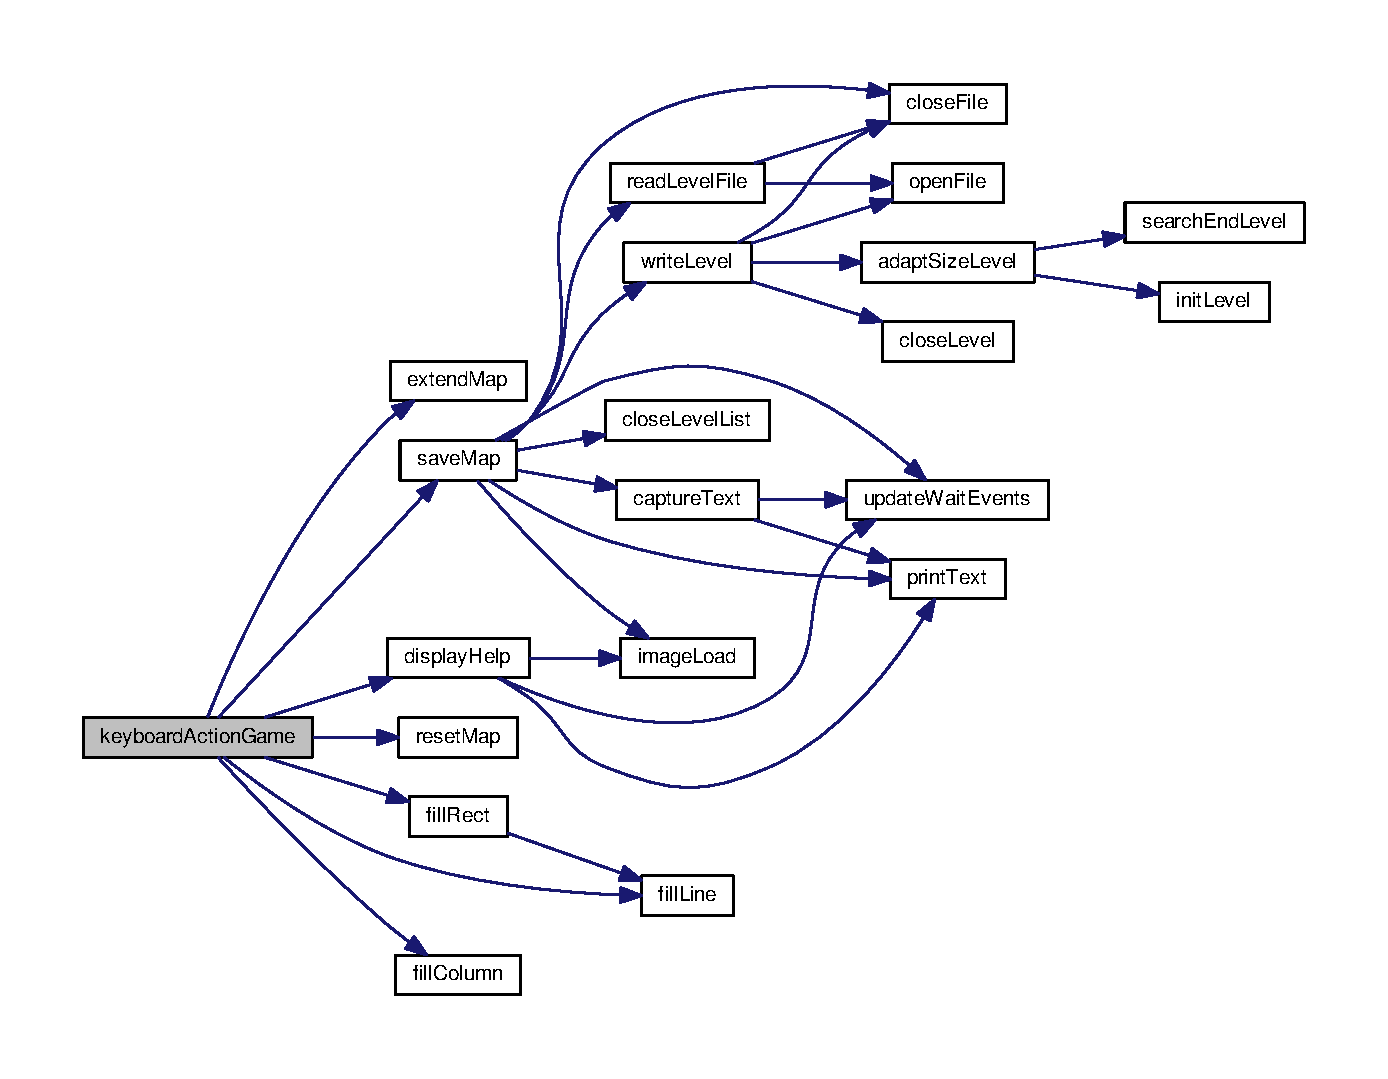
\includegraphics[width=350pt]{input_8c_a0f2aa7e2cd7674e43532893e4f2802e8_cgraph}
\end{center}
\end{figure}


\hypertarget{input_8c_aac9044909637f02a277d101651e126a7}{\index{input.\-c@{input.\-c}!keyboard\-Action\-Menu@{keyboard\-Action\-Menu}}
\index{keyboard\-Action\-Menu@{keyboard\-Action\-Menu}!input.c@{input.\-c}}
\paragraph[{keyboard\-Action\-Menu}]{\setlength{\rightskip}{0pt plus 5cm}void keyboard\-Action\-Menu (
\begin{DoxyParamCaption}
\item[{{\bf Input} $\ast$}]{in, }
\item[{int $\ast$}]{cursor\-Pos, }
\item[{int $\ast$}]{select, }
\item[{int}]{nb\-\_\-options}
\end{DoxyParamCaption}
)}}\label{input_8c_aac9044909637f02a277d101651e126a7}
perform menu action commanded by keyboard action 
\begin{DoxyParams}[1]{Parameters}
\mbox{\tt in}  & {\em in} & the input structure \\
\hline
\mbox{\tt out}  & {\em cursor\-Pos} & the cursor position \\
\hline
\mbox{\tt out}  & {\em select} & boolean about selecting the option or quit to title screen \\
\hline
\mbox{\tt in}  & {\em nb\-\_\-options} & the number of options of the menu \\
\hline
\end{DoxyParams}
\hypertarget{input_8c_a907831170dedec3a0af4e4b1e178b854}{\index{input.\-c@{input.\-c}!update\-Events@{update\-Events}}
\index{update\-Events@{update\-Events}!input.c@{input.\-c}}
\paragraph[{update\-Events}]{\setlength{\rightskip}{0pt plus 5cm}void update\-Events (
\begin{DoxyParamCaption}
\item[{{\bf Input} $\ast$}]{in}
\end{DoxyParamCaption}
)}}\label{input_8c_a907831170dedec3a0af4e4b1e178b854}
get keyboard input with a S\-D\-L\-\_\-\-Poll\-Event 
\begin{DoxyParams}[1]{Parameters}
\mbox{\tt out}  & {\em in} & the input structure \\
\hline
\end{DoxyParams}
\hypertarget{input_8c_ad3310b398fa046500863c183fd4468e6}{\index{input.\-c@{input.\-c}!update\-Wait\-Events@{update\-Wait\-Events}}
\index{update\-Wait\-Events@{update\-Wait\-Events}!input.c@{input.\-c}}
\paragraph[{update\-Wait\-Events}]{\setlength{\rightskip}{0pt plus 5cm}int update\-Wait\-Events (
\begin{DoxyParamCaption}
\item[{{\bf Input} $\ast$}]{in}
\end{DoxyParamCaption}
)}}\label{input_8c_ad3310b398fa046500863c183fd4468e6}
get keyboard input with a S\-D\-L\-\_\-\-Wait\-Event 
\begin{DoxyParams}[1]{Parameters}
\mbox{\tt out}  & {\em in} & the input structure \\
\hline
\end{DoxyParams}
\begin{DoxyReturn}{Returns}
1 if a key is activated 
\end{DoxyReturn}

\hypertarget{main_8c}{\subsection{main.\-c File Reference}
\label{main_8c}\index{main.\-c@{main.\-c}}
}
{\ttfamily \#include \char`\"{}game.\-h\char`\"{}}\\*
{\ttfamily \#include \char`\"{}const.\-h\char`\"{}}\\*
{\ttfamily \#include \char`\"{}menu.\-h\char`\"{}}\\*
{\ttfamily \#include \char`\"{}menu\-\_\-level.\-h\char`\"{}}\\*
{\ttfamily \#include \char`\"{}menu\-\_\-option.\-h\char`\"{}}\\*
{\ttfamily \#include \char`\"{}option.\-h\char`\"{}}\\*
\subsubsection*{Functions}
\begin{DoxyCompactItemize}
\item 
int \hyperlink{main_8c_a0ddf1224851353fc92bfbff6f499fa97}{main} (int argc, char $\ast$argv\mbox{[}$\,$\mbox{]})
\end{DoxyCompactItemize}


\subsubsection{Detailed Description}
\begin{DoxyAuthor}{Author}
Xavier C\-O\-P\-O\-N\-E\-T 
\end{DoxyAuthor}
\begin{DoxyDate}{Date}
2014-\/02-\/27 
\end{DoxyDate}


\subsubsection{Function Documentation}
\hypertarget{main_8c_a0ddf1224851353fc92bfbff6f499fa97}{\index{main.\-c@{main.\-c}!main@{main}}
\index{main@{main}!main.c@{main.\-c}}
\paragraph[{main}]{\setlength{\rightskip}{0pt plus 5cm}int main (
\begin{DoxyParamCaption}
\item[{int}]{argc, }
\item[{char $\ast$}]{argv\mbox{[}$\,$\mbox{]}}
\end{DoxyParamCaption}
)}}\label{main_8c_a0ddf1224851353fc92bfbff6f499fa97}
Main 
\begin{DoxyParams}[1]{Parameters}
\mbox{\tt in,out}  & {\em argc} & argc \\
\hline
\mbox{\tt in,out}  & {\em argv} & argv \\
\hline
\end{DoxyParams}


Here is the call graph for this function\-:
\nopagebreak
\begin{figure}[H]
\begin{center}
\leavevmode
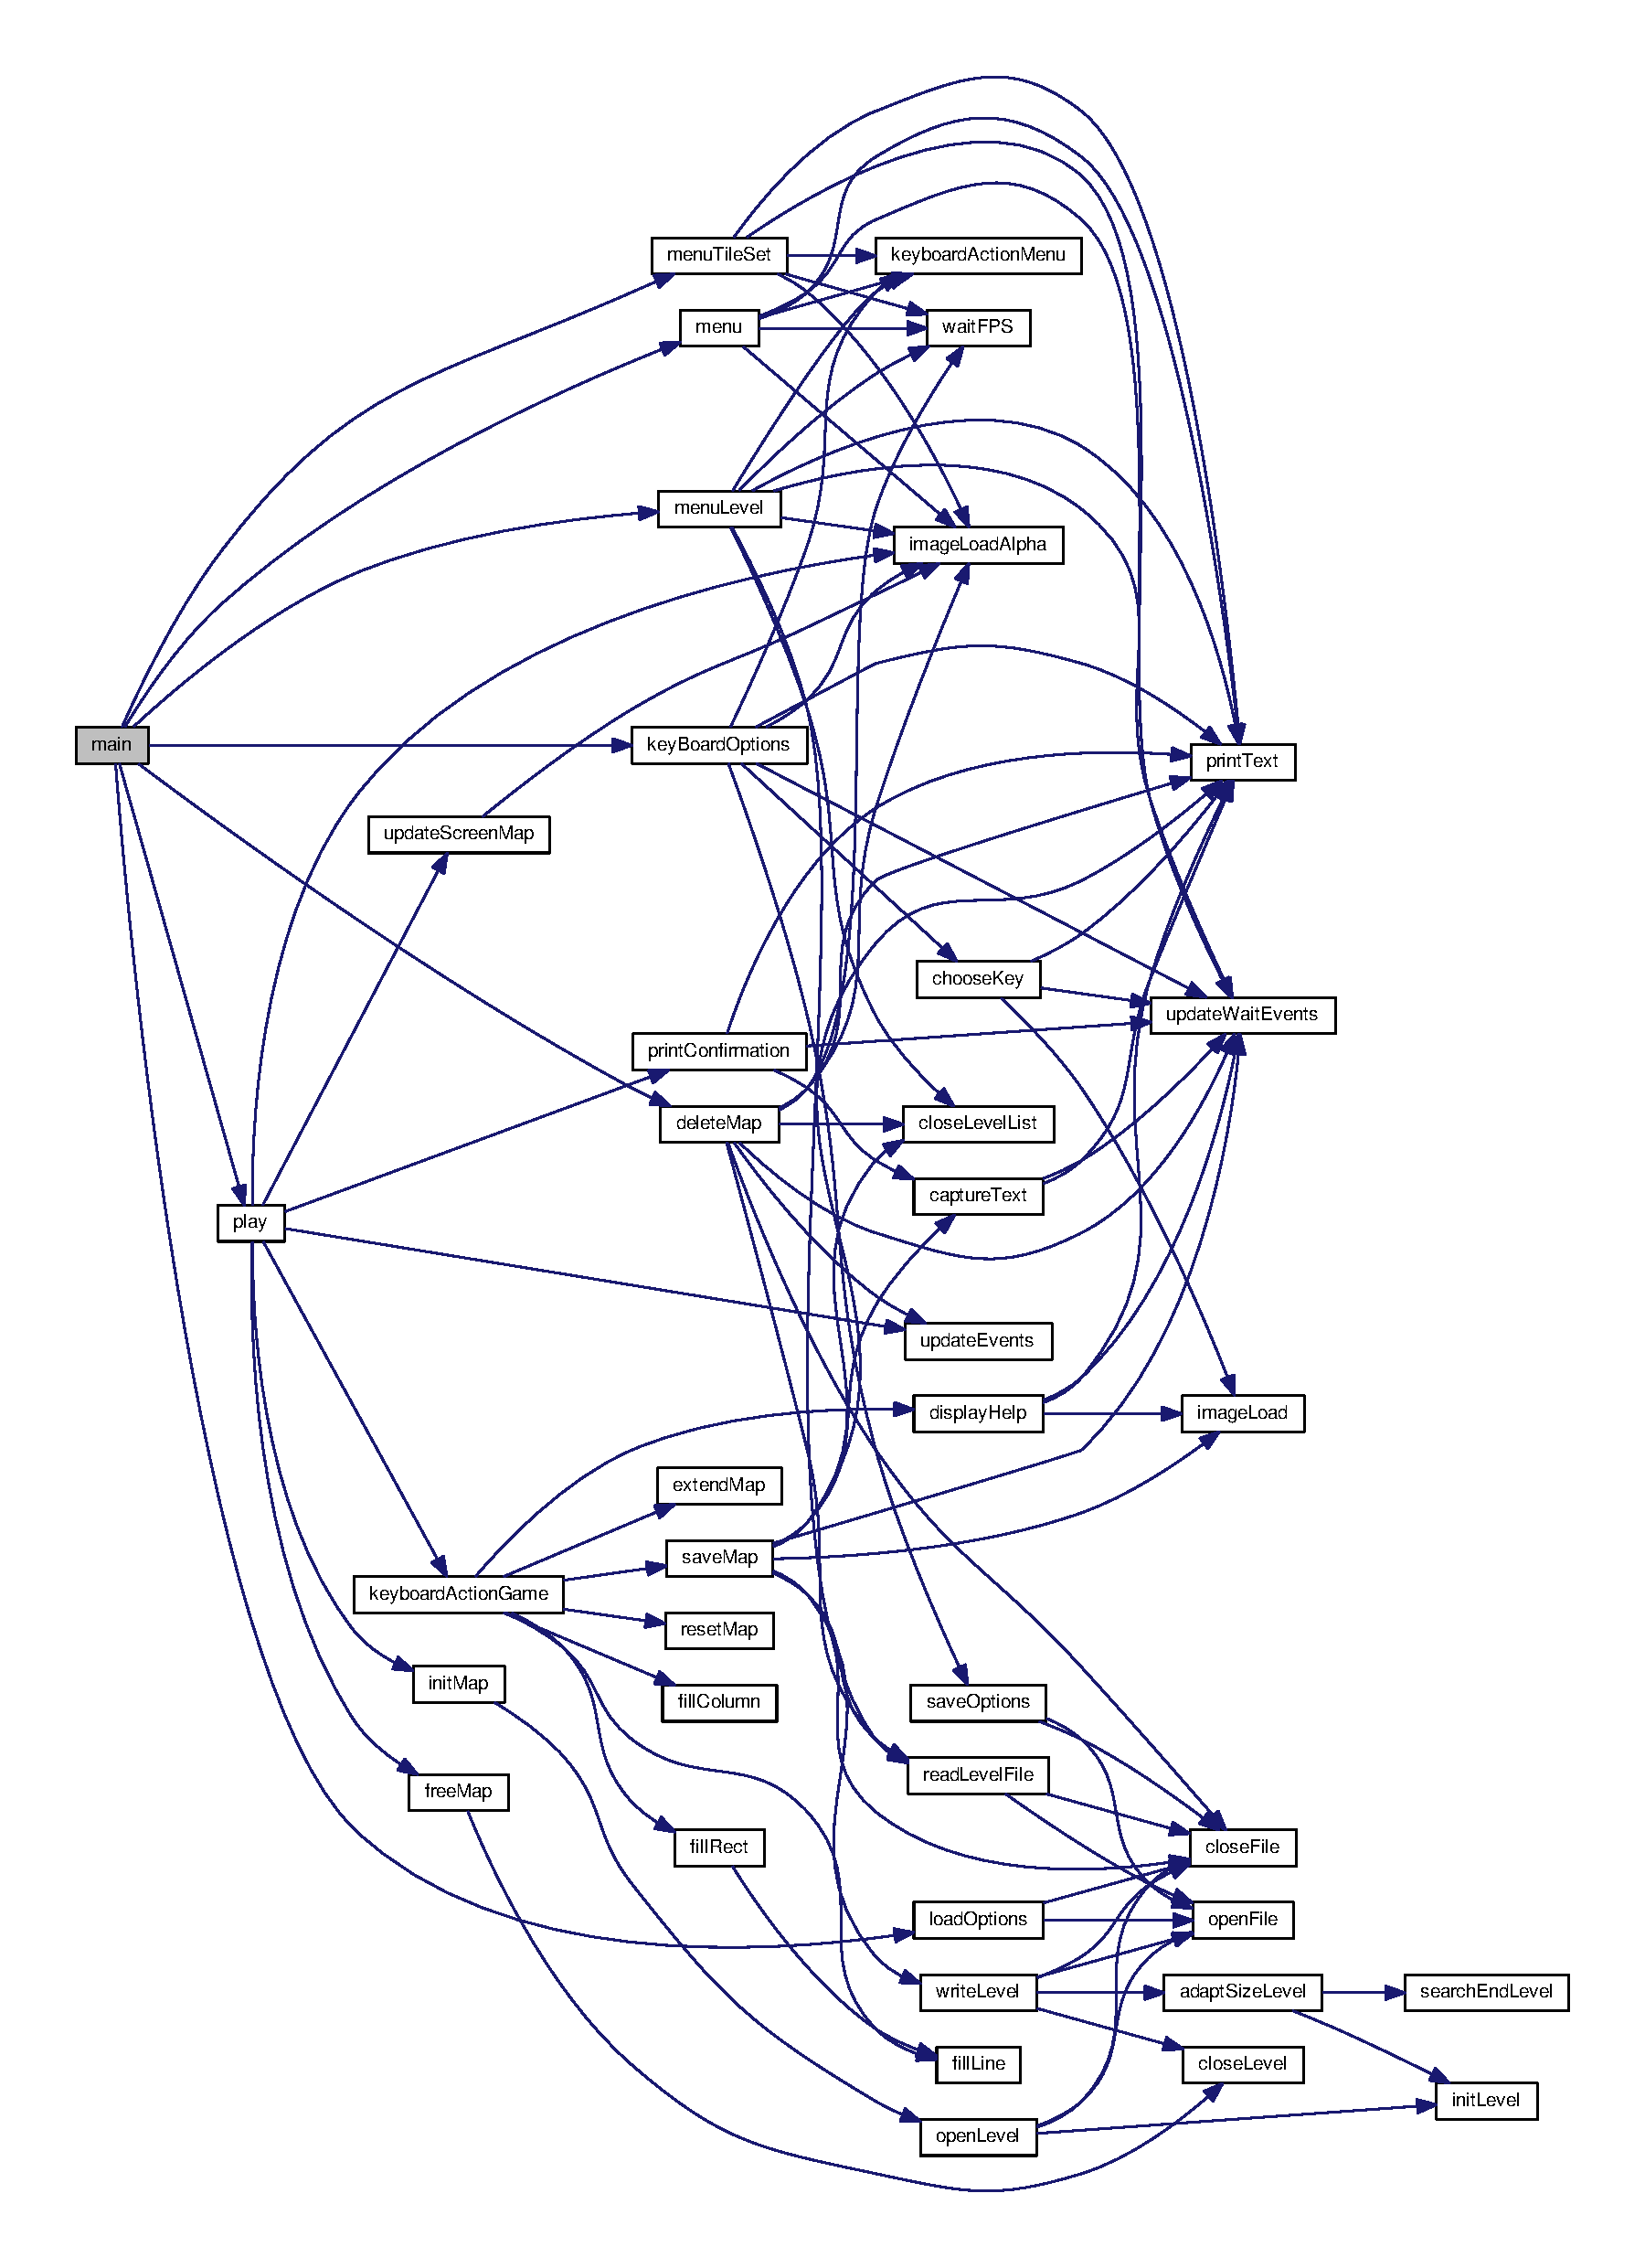
\includegraphics[width=350pt]{main_8c_a0ddf1224851353fc92bfbff6f499fa97_cgraph}
\end{center}
\end{figure}



\hypertarget{map_8c}{\subsection{map.\-c File Reference}
\label{map_8c}\index{map.\-c@{map.\-c}}
}


loading and displaying the map  


{\ttfamily \#include \char`\"{}map.\-h\char`\"{}}\\*
\subsubsection*{Functions}
\begin{DoxyCompactItemize}
\item 
void \hyperlink{map_8c_afc8482e2afe6f96b7d6cb6ce3fc7081c}{update\-Screen\-Map} (S\-D\-L\-\_\-\-Surface $\ast$screen, \hyperlink{struct_map}{Map} $\ast$m, char $\ast$tileset)
\item 
void \hyperlink{map_8c_a6f031e5ad35ada9038d3a72a56053760}{scrolling} (\hyperlink{struct_map}{Map} $\ast$m, int direction, float speed)
\item 
\hyperlink{struct_map}{Map} $\ast$ \hyperlink{map_8c_ace46be3df708e41a326676e6ad122bcc}{init\-Map} (S\-D\-L\-\_\-\-Surface $\ast$screen, char $\ast$level\-\_\-name, \hyperlink{structlist}{list} $\ast$l, \hyperlink{structplatform_set}{platform\-Set} $\ast$ps)
\item 
void \hyperlink{map_8c_ac8d4dd6fc80c79d9cb5899684740d074}{free\-Map} (\hyperlink{struct_map}{Map} $\ast$m)
\item 
int \hyperlink{map_8c_abf181167fafe365865bf0468959f1426}{collision\-Map} (S\-D\-L\-\_\-\-Rect r, \hyperlink{struct_map}{Map} $\ast$m, int type)
\end{DoxyCompactItemize}


\subsubsection{Detailed Description}
loading and displaying the map \begin{DoxyAuthor}{Author}
Xavier C\-O\-P\-O\-N\-E\-T 
\end{DoxyAuthor}
\begin{DoxyDate}{Date}
2014-\/03-\/18 
\end{DoxyDate}


\subsubsection{Function Documentation}
\hypertarget{map_8c_abf181167fafe365865bf0468959f1426}{\index{map.\-c@{map.\-c}!collision\-Map@{collision\-Map}}
\index{collision\-Map@{collision\-Map}!map.c@{map.\-c}}
\paragraph[{collision\-Map}]{\setlength{\rightskip}{0pt plus 5cm}int collision\-Map (
\begin{DoxyParamCaption}
\item[{S\-D\-L\-\_\-\-Rect}]{r, }
\item[{{\bf Map} $\ast$}]{m, }
\item[{int}]{type}
\end{DoxyParamCaption}
)}}\label{map_8c_abf181167fafe365865bf0468959f1426}
determine if there is a collision beteewen a sprite and a \char`\"{}wall\char`\"{} of the map 
\begin{DoxyParams}[1]{Parameters}
\mbox{\tt in}  & {\em r} & S\-D\-L\-\_\-\-Rect corresponding to the sprite \\
\hline
\mbox{\tt in}  & {\em m} & map \\
\hline
\mbox{\tt in}  & {\em type} & 0 if not a projectile \\
\hline
\end{DoxyParams}
\begin{DoxyReturn}{Returns}
1 if there is a collision, 0 if not,2 if collision with star/coin, 3 if spring 
\end{DoxyReturn}


Here is the call graph for this function\-:\nopagebreak
\begin{figure}[H]
\begin{center}
\leavevmode
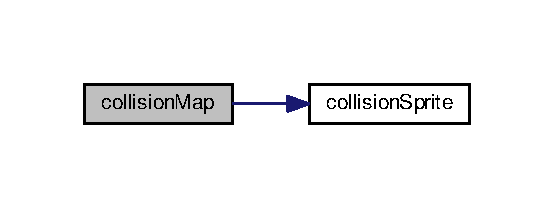
\includegraphics[width=266pt]{map_8c_abf181167fafe365865bf0468959f1426_cgraph}
\end{center}
\end{figure}


\hypertarget{map_8c_ac8d4dd6fc80c79d9cb5899684740d074}{\index{map.\-c@{map.\-c}!free\-Map@{free\-Map}}
\index{free\-Map@{free\-Map}!map.c@{map.\-c}}
\paragraph[{free\-Map}]{\setlength{\rightskip}{0pt plus 5cm}void free\-Map (
\begin{DoxyParamCaption}
\item[{{\bf Map} $\ast$}]{m}
\end{DoxyParamCaption}
)}}\label{map_8c_ac8d4dd6fc80c79d9cb5899684740d074}
free memory allocated to the map 
\begin{DoxyParams}[1]{Parameters}
\mbox{\tt in,out}  & {\em m} & the map \\
\hline
\end{DoxyParams}


Here is the call graph for this function\-:\nopagebreak
\begin{figure}[H]
\begin{center}
\leavevmode
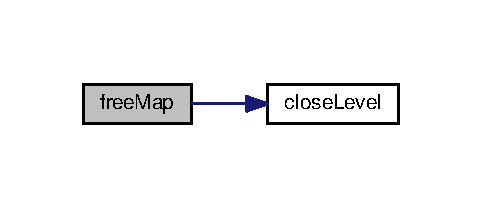
\includegraphics[width=232pt]{map_8c_ac8d4dd6fc80c79d9cb5899684740d074_cgraph}
\end{center}
\end{figure}


\hypertarget{map_8c_ace46be3df708e41a326676e6ad122bcc}{\index{map.\-c@{map.\-c}!init\-Map@{init\-Map}}
\index{init\-Map@{init\-Map}!map.c@{map.\-c}}
\paragraph[{init\-Map}]{\setlength{\rightskip}{0pt plus 5cm}{\bf Map} $\ast$ init\-Map (
\begin{DoxyParamCaption}
\item[{S\-D\-L\-\_\-\-Surface $\ast$}]{screen, }
\item[{char $\ast$}]{level\-\_\-name, }
\item[{{\bf list} $\ast$}]{l, }
\item[{{\bf platform\-Set} $\ast$}]{ps}
\end{DoxyParamCaption}
)}}\label{map_8c_ace46be3df708e41a326676e6ad122bcc}
initialize the map 
\begin{DoxyParams}[1]{Parameters}
\mbox{\tt in}  & {\em screen} & game screen \\
\hline
\mbox{\tt in}  & {\em level\-\_\-name} & lvl name \\
\hline
\mbox{\tt out}  & {\em l} & the enemy list that stocks the enemies \\
\hline
\mbox{\tt out}  & {\em ps} & the platform set for the mobile platforms \\
\hline
\end{DoxyParams}
\begin{DoxyReturn}{Returns}
pointer on the map 
\end{DoxyReturn}


Here is the call graph for this function\-:\nopagebreak
\begin{figure}[H]
\begin{center}
\leavevmode
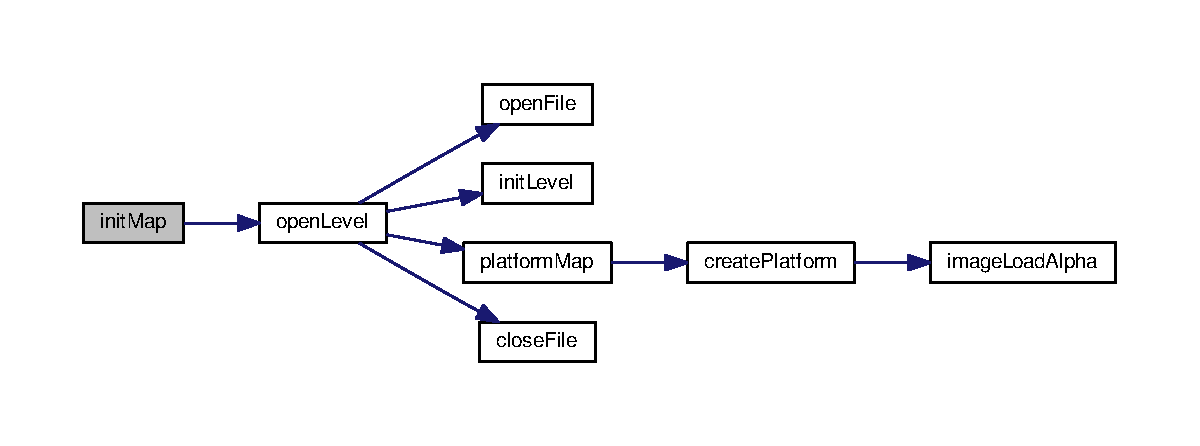
\includegraphics[width=350pt]{map_8c_ace46be3df708e41a326676e6ad122bcc_cgraph}
\end{center}
\end{figure}


\hypertarget{map_8c_a6f031e5ad35ada9038d3a72a56053760}{\index{map.\-c@{map.\-c}!scrolling@{scrolling}}
\index{scrolling@{scrolling}!map.c@{map.\-c}}
\paragraph[{scrolling}]{\setlength{\rightskip}{0pt plus 5cm}void scrolling (
\begin{DoxyParamCaption}
\item[{{\bf Map} $\ast$}]{m, }
\item[{int}]{direction, }
\item[{float}]{speed}
\end{DoxyParamCaption}
)}}\label{map_8c_a6f031e5ad35ada9038d3a72a56053760}
scroll the map 
\begin{DoxyParams}[1]{Parameters}
\mbox{\tt in,out}  & {\em m} & the lvl \\
\hline
\mbox{\tt in}  & {\em direction} & scrolling direction \\
\hline
\mbox{\tt in}  & {\em speed} & scrolling speed \\
\hline
\end{DoxyParams}
\hypertarget{map_8c_afc8482e2afe6f96b7d6cb6ce3fc7081c}{\index{map.\-c@{map.\-c}!update\-Screen\-Map@{update\-Screen\-Map}}
\index{update\-Screen\-Map@{update\-Screen\-Map}!map.c@{map.\-c}}
\paragraph[{update\-Screen\-Map}]{\setlength{\rightskip}{0pt plus 5cm}void update\-Screen\-Map (
\begin{DoxyParamCaption}
\item[{S\-D\-L\-\_\-\-Surface $\ast$}]{screen, }
\item[{{\bf Map} $\ast$}]{m, }
\item[{char $\ast$}]{tileset}
\end{DoxyParamCaption}
)}}\label{map_8c_afc8482e2afe6f96b7d6cb6ce3fc7081c}
update and display the map 
\begin{DoxyParams}[1]{Parameters}
\mbox{\tt in,out}  & {\em screen} & \\
\hline
\mbox{\tt in}  & {\em m} & The map \\
\hline
\mbox{\tt in}  & {\em tileset} & the level tileset \\
\hline
\end{DoxyParams}


Here is the call graph for this function\-:\nopagebreak
\begin{figure}[H]
\begin{center}
\leavevmode
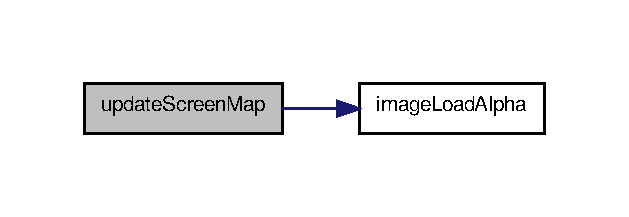
\includegraphics[width=302pt]{map_8c_afc8482e2afe6f96b7d6cb6ce3fc7081c_cgraph}
\end{center}
\end{figure}



\hypertarget{map_8h}{\subsection{map.\-h File Reference}
\label{map_8h}\index{map.\-h@{map.\-h}}
}


\hyperlink{map_8c}{map.\-c} header  


{\ttfamily \#include $<$stdlib.\-h$>$}\\*
{\ttfamily \#include $<$stdio.\-h$>$}\\*
{\ttfamily \#include $<$errno.\-h$>$}\\*
{\ttfamily \#include $<$S\-D\-L/\-S\-D\-L.\-h$>$}\\*
{\ttfamily \#include $<$S\-D\-L/\-S\-D\-L\-\_\-image.\-h$>$}\\*
{\ttfamily \#include \char`\"{}image.\-h\char`\"{}}\\*
{\ttfamily \#include \char`\"{}file\-\_\-level.\-h\char`\"{}}\\*
\subsubsection*{Functions}
\begin{DoxyCompactItemize}
\item 
void \hyperlink{map_8h_afc8482e2afe6f96b7d6cb6ce3fc7081c}{update\-Screen\-Map} (S\-D\-L\-\_\-\-Surface $\ast$screen, \hyperlink{struct_map}{Map} $\ast$m, char $\ast$tileset)
\item 
void \hyperlink{map_8h_a6f031e5ad35ada9038d3a72a56053760}{scrolling} (\hyperlink{struct_map}{Map} $\ast$m, int direction, float speed)
\item 
\hyperlink{struct_map}{Map} $\ast$ \hyperlink{map_8h_a4e2ce263b91d4c8915e26d5792e10747}{init\-Map} (S\-D\-L\-\_\-\-Surface $\ast$screen, char $\ast$level\-\_\-name, \hyperlink{structlist}{list} $\ast$l, \hyperlink{structplatform_set}{platform\-Set} $\ast$ps)
\item 
void \hyperlink{map_8h_ac8d4dd6fc80c79d9cb5899684740d074}{free\-Map} (\hyperlink{struct_map}{Map} $\ast$m)
\item 
int \hyperlink{map_8h_abf181167fafe365865bf0468959f1426}{collision\-Map} (S\-D\-L\-\_\-\-Rect r, \hyperlink{struct_map}{Map} $\ast$m, int type)
\end{DoxyCompactItemize}


\subsubsection{Detailed Description}
\hyperlink{map_8c}{map.\-c} header \begin{DoxyAuthor}{Author}
Xavier C\-O\-P\-O\-N\-E\-T 
\end{DoxyAuthor}
\begin{DoxyDate}{Date}
2014-\/03-\/18 
\end{DoxyDate}


\subsubsection{Function Documentation}
\hypertarget{map_8h_abf181167fafe365865bf0468959f1426}{\index{map.\-h@{map.\-h}!collision\-Map@{collision\-Map}}
\index{collision\-Map@{collision\-Map}!map.h@{map.\-h}}
\paragraph[{collision\-Map}]{\setlength{\rightskip}{0pt plus 5cm}int collision\-Map (
\begin{DoxyParamCaption}
\item[{S\-D\-L\-\_\-\-Rect}]{r, }
\item[{{\bf Map} $\ast$}]{m, }
\item[{int}]{type}
\end{DoxyParamCaption}
)}}\label{map_8h_abf181167fafe365865bf0468959f1426}
determine if there is a collision beteewen a sprite and a \char`\"{}wall\char`\"{} of the map 
\begin{DoxyParams}[1]{Parameters}
\mbox{\tt in}  & {\em r} & S\-D\-L\-\_\-\-Rect corresponding to the sprite \\
\hline
\mbox{\tt in}  & {\em m} & map \\
\hline
\mbox{\tt in}  & {\em type} & 0 if not a projectile \\
\hline
\end{DoxyParams}
\begin{DoxyReturn}{Returns}
1 if there is a collision, 0 if not,2 if collision with star/coin, 3 if spring 
\end{DoxyReturn}


Here is the call graph for this function\-:\nopagebreak
\begin{figure}[H]
\begin{center}
\leavevmode
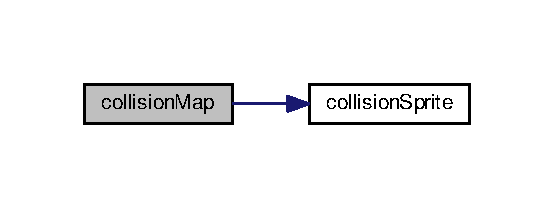
\includegraphics[width=266pt]{map_8h_abf181167fafe365865bf0468959f1426_cgraph}
\end{center}
\end{figure}


\hypertarget{map_8h_ac8d4dd6fc80c79d9cb5899684740d074}{\index{map.\-h@{map.\-h}!free\-Map@{free\-Map}}
\index{free\-Map@{free\-Map}!map.h@{map.\-h}}
\paragraph[{free\-Map}]{\setlength{\rightskip}{0pt plus 5cm}void free\-Map (
\begin{DoxyParamCaption}
\item[{{\bf Map} $\ast$}]{m}
\end{DoxyParamCaption}
)}}\label{map_8h_ac8d4dd6fc80c79d9cb5899684740d074}
free memory allocated to the map 
\begin{DoxyParams}[1]{Parameters}
\mbox{\tt in,out}  & {\em m} & the map \\
\hline
\end{DoxyParams}


Here is the call graph for this function\-:\nopagebreak
\begin{figure}[H]
\begin{center}
\leavevmode
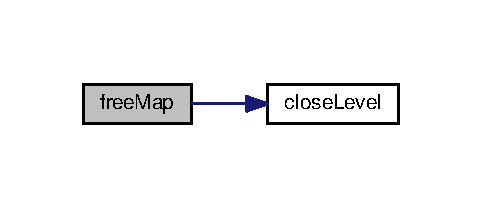
\includegraphics[width=232pt]{map_8h_ac8d4dd6fc80c79d9cb5899684740d074_cgraph}
\end{center}
\end{figure}


\hypertarget{map_8h_a4e2ce263b91d4c8915e26d5792e10747}{\index{map.\-h@{map.\-h}!init\-Map@{init\-Map}}
\index{init\-Map@{init\-Map}!map.h@{map.\-h}}
\paragraph[{init\-Map}]{\setlength{\rightskip}{0pt plus 5cm}{\bf Map}$\ast$ init\-Map (
\begin{DoxyParamCaption}
\item[{S\-D\-L\-\_\-\-Surface $\ast$}]{screen, }
\item[{char $\ast$}]{level\-\_\-name, }
\item[{{\bf list} $\ast$}]{l, }
\item[{{\bf platform\-Set} $\ast$}]{ps}
\end{DoxyParamCaption}
)}}\label{map_8h_a4e2ce263b91d4c8915e26d5792e10747}
initialize the map 
\begin{DoxyParams}[1]{Parameters}
\mbox{\tt in}  & {\em screen} & game screen \\
\hline
\mbox{\tt in}  & {\em level\-\_\-name} & lvl name \\
\hline
\mbox{\tt out}  & {\em l} & the enemy list that stocks the enemies \\
\hline
\mbox{\tt out}  & {\em ps} & the platform set for the mobile platforms \\
\hline
\end{DoxyParams}
\begin{DoxyReturn}{Returns}
pointer on the map 
\end{DoxyReturn}


Here is the call graph for this function\-:\nopagebreak
\begin{figure}[H]
\begin{center}
\leavevmode
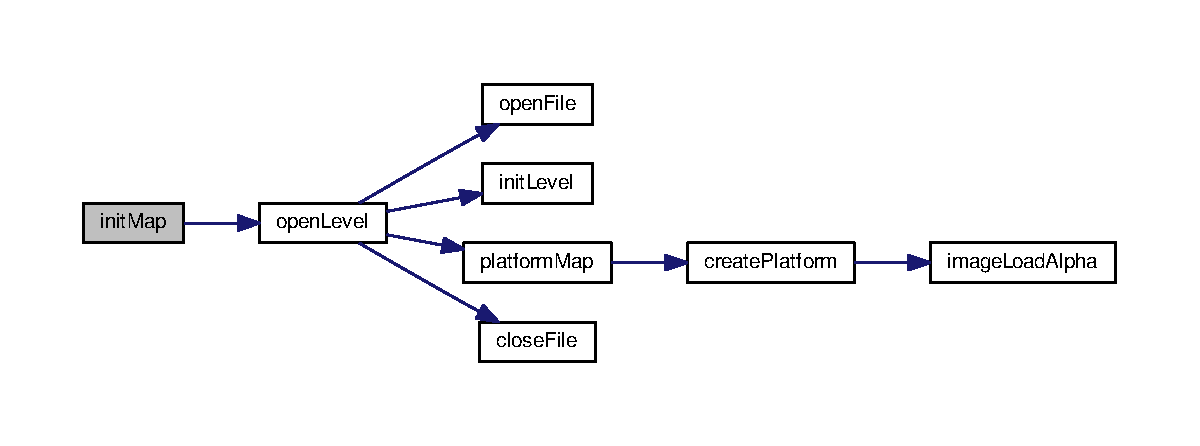
\includegraphics[width=350pt]{map_8h_a4e2ce263b91d4c8915e26d5792e10747_cgraph}
\end{center}
\end{figure}


\hypertarget{map_8h_a6f031e5ad35ada9038d3a72a56053760}{\index{map.\-h@{map.\-h}!scrolling@{scrolling}}
\index{scrolling@{scrolling}!map.h@{map.\-h}}
\paragraph[{scrolling}]{\setlength{\rightskip}{0pt plus 5cm}void scrolling (
\begin{DoxyParamCaption}
\item[{{\bf Map} $\ast$}]{m, }
\item[{int}]{direction, }
\item[{float}]{speed}
\end{DoxyParamCaption}
)}}\label{map_8h_a6f031e5ad35ada9038d3a72a56053760}
scroll the map 
\begin{DoxyParams}[1]{Parameters}
\mbox{\tt in,out}  & {\em m} & the lvl \\
\hline
\mbox{\tt in}  & {\em direction} & scrolling direction \\
\hline
\mbox{\tt in}  & {\em speed} & scrolling speed \\
\hline
\end{DoxyParams}
\hypertarget{map_8h_afc8482e2afe6f96b7d6cb6ce3fc7081c}{\index{map.\-h@{map.\-h}!update\-Screen\-Map@{update\-Screen\-Map}}
\index{update\-Screen\-Map@{update\-Screen\-Map}!map.h@{map.\-h}}
\paragraph[{update\-Screen\-Map}]{\setlength{\rightskip}{0pt plus 5cm}void update\-Screen\-Map (
\begin{DoxyParamCaption}
\item[{S\-D\-L\-\_\-\-Surface $\ast$}]{screen, }
\item[{{\bf Map} $\ast$}]{m, }
\item[{char $\ast$}]{tileset}
\end{DoxyParamCaption}
)}}\label{map_8h_afc8482e2afe6f96b7d6cb6ce3fc7081c}
update and display the map 
\begin{DoxyParams}[1]{Parameters}
\mbox{\tt in,out}  & {\em screen} & \\
\hline
\mbox{\tt in}  & {\em m} & The map \\
\hline
\mbox{\tt in}  & {\em tileset} & the level tileset \\
\hline
\end{DoxyParams}


Here is the call graph for this function\-:\nopagebreak
\begin{figure}[H]
\begin{center}
\leavevmode
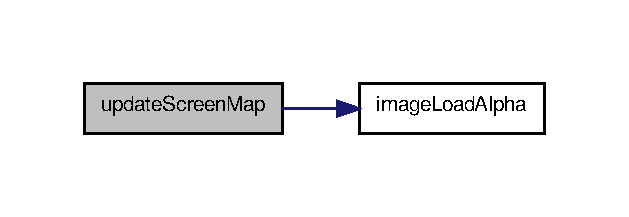
\includegraphics[width=302pt]{map_8h_afc8482e2afe6f96b7d6cb6ce3fc7081c_cgraph}
\end{center}
\end{figure}



\hypertarget{menu_8c}{\subsection{menu.\-c File Reference}
\label{menu_8c}\index{menu.\-c@{menu.\-c}}
}


Contain the main menu management.  


{\ttfamily \#include \char`\"{}menu.\-h\char`\"{}}\\*
\subsubsection*{Functions}
\begin{DoxyCompactItemize}
\item 
int \hyperlink{menu_8c_a9b210afb32784dfdf07bd2d4ef25e0bc}{menu} (S\-D\-L\-\_\-\-Surface $\ast$screen, int $\ast$choice, int $\ast$go)
\item 
int \hyperlink{menu_8c_a2e385684b2e6cc22168f98525f3693d8}{menu\-Tile\-Set} (S\-D\-L\-\_\-\-Surface $\ast$screen, char tile\-Set\-\_\-name\mbox{[}\hyperlink{const_8h_a9620725a4f8ab39e0912adede7cb347f}{M\-A\-X\-\_\-\-L\-E\-N\-G\-T\-H\-\_\-\-F\-I\-L\-E\-\_\-\-N\-A\-M\-E}\mbox{]})
\end{DoxyCompactItemize}


\subsubsection{Detailed Description}
Contain the main menu management. \begin{DoxyAuthor}{Author}
Glenn H\-E\-R\-R\-O\-U 
\end{DoxyAuthor}
\begin{DoxyDate}{Date}
2014-\/04-\/20 
\end{DoxyDate}


\subsubsection{Function Documentation}
\hypertarget{menu_8c_a9b210afb32784dfdf07bd2d4ef25e0bc}{\index{menu.\-c@{menu.\-c}!menu@{menu}}
\index{menu@{menu}!menu.c@{menu.\-c}}
\paragraph[{menu}]{\setlength{\rightskip}{0pt plus 5cm}int menu (
\begin{DoxyParamCaption}
\item[{S\-D\-L\-\_\-\-Surface $\ast$}]{screen, }
\item[{int $\ast$}]{choice, }
\item[{int $\ast$}]{go}
\end{DoxyParamCaption}
)}}\label{menu_8c_a9b210afb32784dfdf07bd2d4ef25e0bc}
Display the menu on the screen 
\begin{DoxyParams}[1]{Parameters}
\mbox{\tt out}  & {\em screen} & the screen of the game \\
\hline
\mbox{\tt out}  & {\em choice} & the option selected \\
\hline
\mbox{\tt out}  & {\em go} & the main loop validation \\
\hline
\end{DoxyParams}
\begin{DoxyReturn}{Returns}
1 if an option has been selected 
\end{DoxyReturn}


Here is the call graph for this function\-:\nopagebreak
\begin{figure}[H]
\begin{center}
\leavevmode
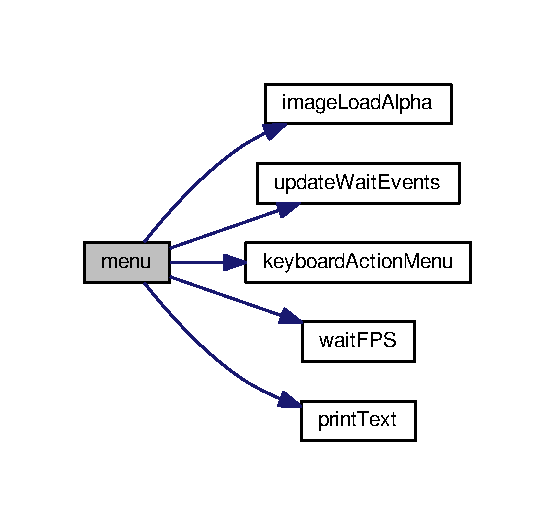
\includegraphics[width=266pt]{menu_8c_a9b210afb32784dfdf07bd2d4ef25e0bc_cgraph}
\end{center}
\end{figure}


\hypertarget{menu_8c_a2e385684b2e6cc22168f98525f3693d8}{\index{menu.\-c@{menu.\-c}!menu\-Tile\-Set@{menu\-Tile\-Set}}
\index{menu\-Tile\-Set@{menu\-Tile\-Set}!menu.c@{menu.\-c}}
\paragraph[{menu\-Tile\-Set}]{\setlength{\rightskip}{0pt plus 5cm}int menu\-Tile\-Set (
\begin{DoxyParamCaption}
\item[{S\-D\-L\-\_\-\-Surface $\ast$}]{screen, }
\item[{char}]{tile\-Set\-\_\-name\mbox{[}\-M\-A\-X\-\_\-\-L\-E\-N\-G\-T\-H\-\_\-\-F\-I\-L\-E\-\_\-\-N\-A\-M\-E\mbox{]}}
\end{DoxyParamCaption}
)}}\label{menu_8c_a2e385684b2e6cc22168f98525f3693d8}
Display the tileset menu on the screen 
\begin{DoxyParams}[1]{Parameters}
\mbox{\tt out}  & {\em screen} & the screen of the game \\
\hline
\mbox{\tt out}  & {\em tile\-Set\-\_\-name} & The name of the tile\-Set selected \\
\hline
\end{DoxyParams}
\begin{DoxyReturn}{Returns}
1 if a tileset has been selected 
\end{DoxyReturn}


Here is the call graph for this function\-:\nopagebreak
\begin{figure}[H]
\begin{center}
\leavevmode
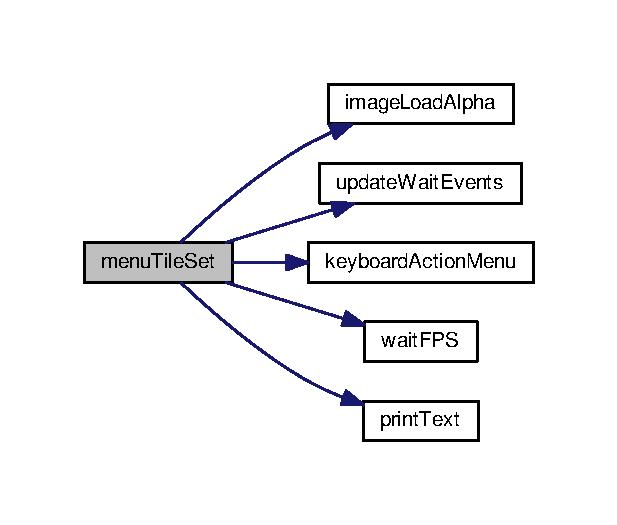
\includegraphics[width=296pt]{menu_8c_a2e385684b2e6cc22168f98525f3693d8_cgraph}
\end{center}
\end{figure}



\hypertarget{menu_8h}{\section{menu.\-h File Reference}
\label{menu_8h}\index{menu.\-h@{menu.\-h}}
}


header de \hyperlink{menu_8c}{menu.\-c}  


{\ttfamily \#include $<$stdlib.\-h$>$}\\*
{\ttfamily \#include $<$stdio.\-h$>$}\\*
{\ttfamily \#include $<$errno.\-h$>$}\\*
{\ttfamily \#include $<$S\-D\-L/\-S\-D\-L.\-h$>$}\\*
{\ttfamily \#include $<$S\-D\-L/\-S\-D\-L\-\_\-image.\-h$>$}\\*
{\ttfamily \#include $<$S\-D\-L/\-S\-D\-L\-\_\-ttf.\-h$>$}\\*
{\ttfamily \#include \char`\"{}const.\-h\char`\"{}}\\*
{\ttfamily \#include \char`\"{}text.\-h\char`\"{}}\\*
{\ttfamily \#include \char`\"{}sound.\-h\char`\"{}}\\*
{\ttfamily \#include \char`\"{}share.\-h\char`\"{}}\\*
Include dependency graph for menu.\-h\-:
\nopagebreak
\begin{figure}[H]
\begin{center}
\leavevmode
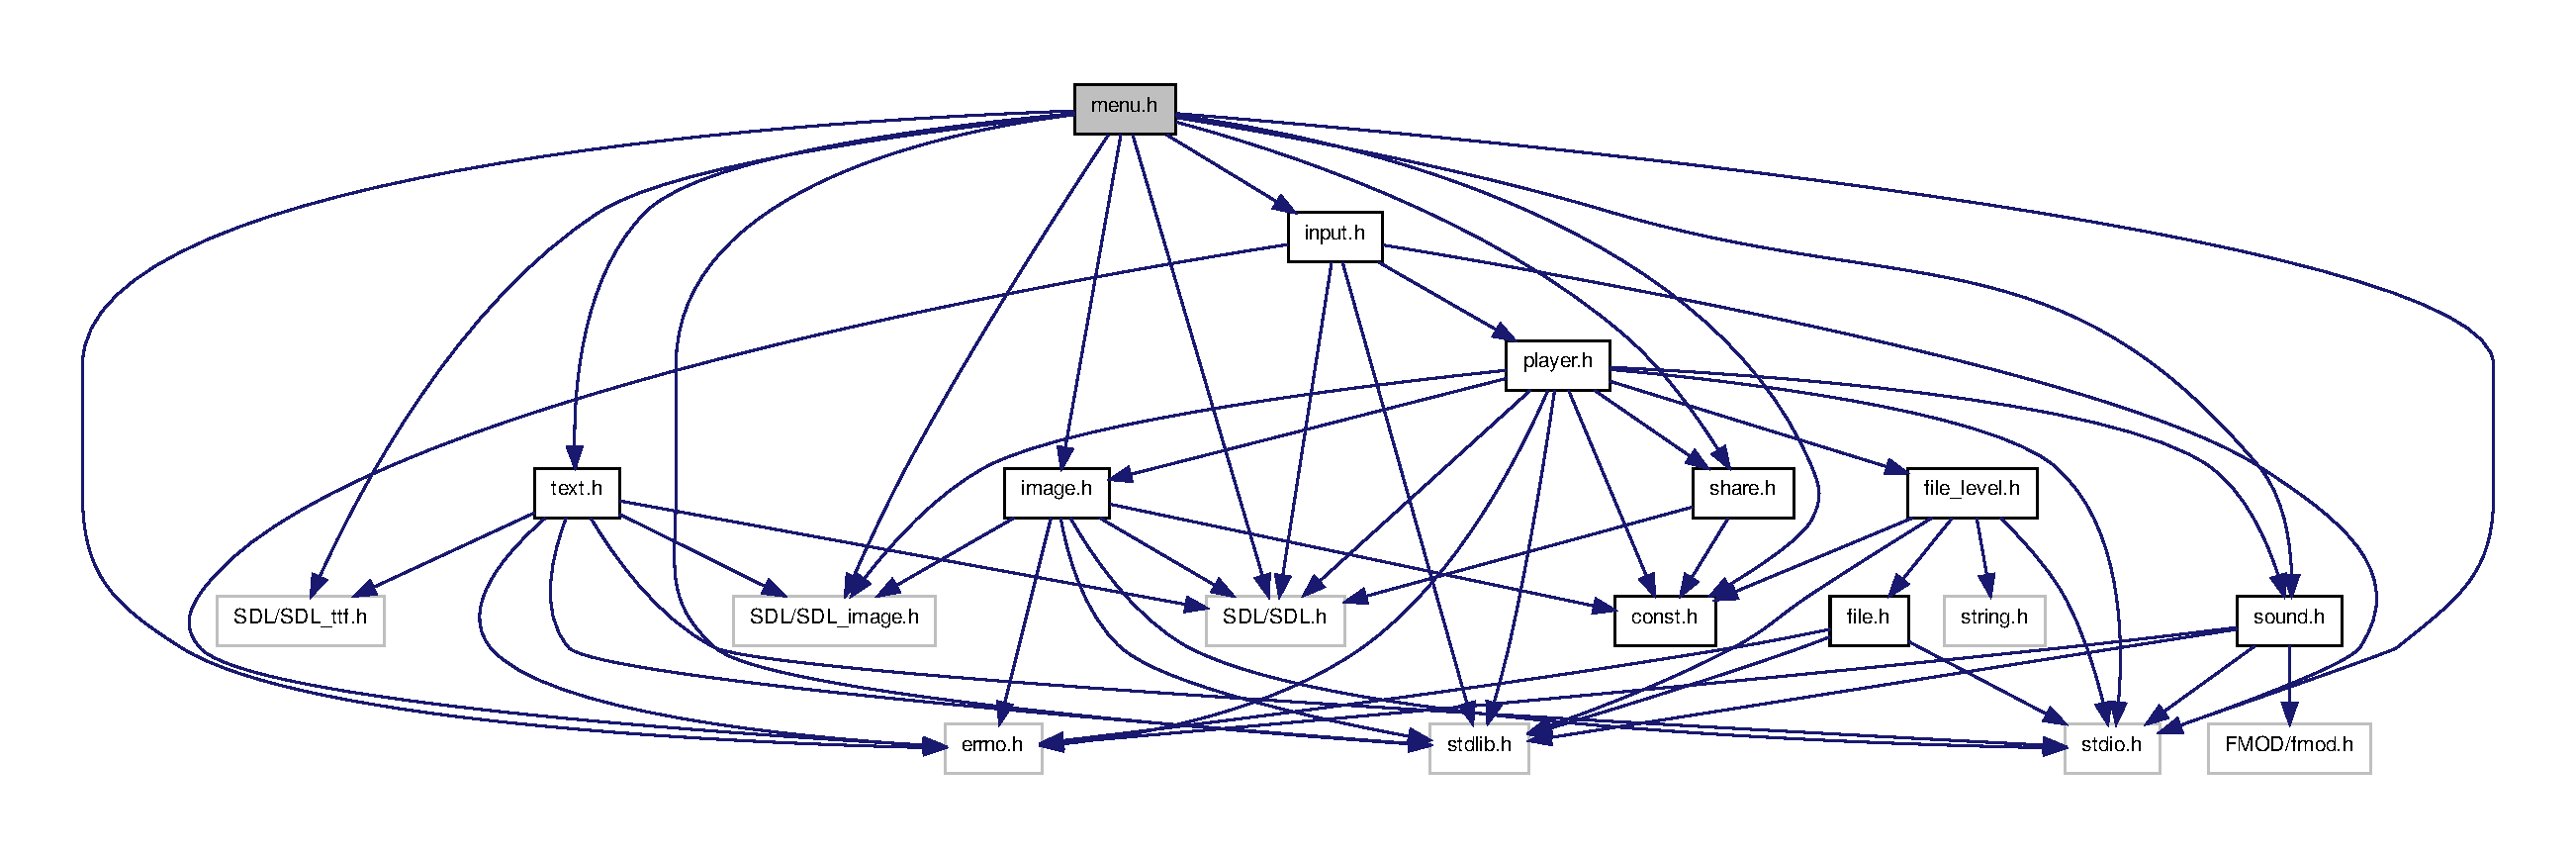
\includegraphics[width=350pt]{menu_8h__incl}
\end{center}
\end{figure}
This graph shows which files directly or indirectly include this file\-:
\nopagebreak
\begin{figure}[H]
\begin{center}
\leavevmode
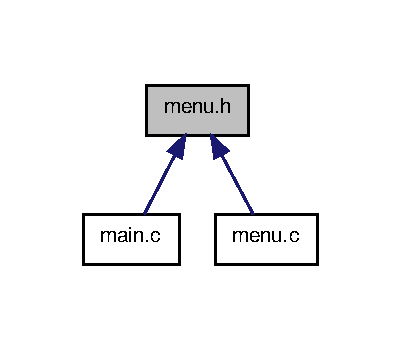
\includegraphics[width=128pt]{menu_8h__dep__incl}
\end{center}
\end{figure}
\subsection*{Functions}
\begin{DoxyCompactItemize}
\item 
\hypertarget{menu_8h_a4604196e3bcbd88eb0a7888effc9dc6f}{int {\bfseries menu} (S\-D\-L\-\_\-\-Surface $\ast$screen, int $\ast$continuer, \hyperlink{struct_sound}{Sound} $\ast$s)}\label{menu_8h_a4604196e3bcbd88eb0a7888effc9dc6f}

\item 
\hypertarget{menu_8h_a0943f574afa5b9e3928862fd99df0d4b}{Uint32 {\bfseries blink\-Text} (Uint32 intervalle, void $\ast$parametre)}\label{menu_8h_a0943f574afa5b9e3928862fd99df0d4b}

\end{DoxyCompactItemize}


\subsection{Detailed Description}
header de \hyperlink{menu_8c}{menu.\-c} \begin{DoxyAuthor}{Author}
Xavier C\-O\-P\-O\-N\-E\-T 
\end{DoxyAuthor}
\begin{DoxyDate}{Date}
2014-\/02-\/27 
\end{DoxyDate}

\hypertarget{menu__level_8c}{\section{menu\-\_\-level.\-c File Reference}
\label{menu__level_8c}\index{menu\-\_\-level.\-c@{menu\-\_\-level.\-c}}
}


level choose menu  


{\ttfamily \#include \char`\"{}menu\-\_\-level.\-h\char`\"{}}\\*
Include dependency graph for menu\-\_\-level.\-c\-:
\nopagebreak
\begin{figure}[H]
\begin{center}
\leavevmode
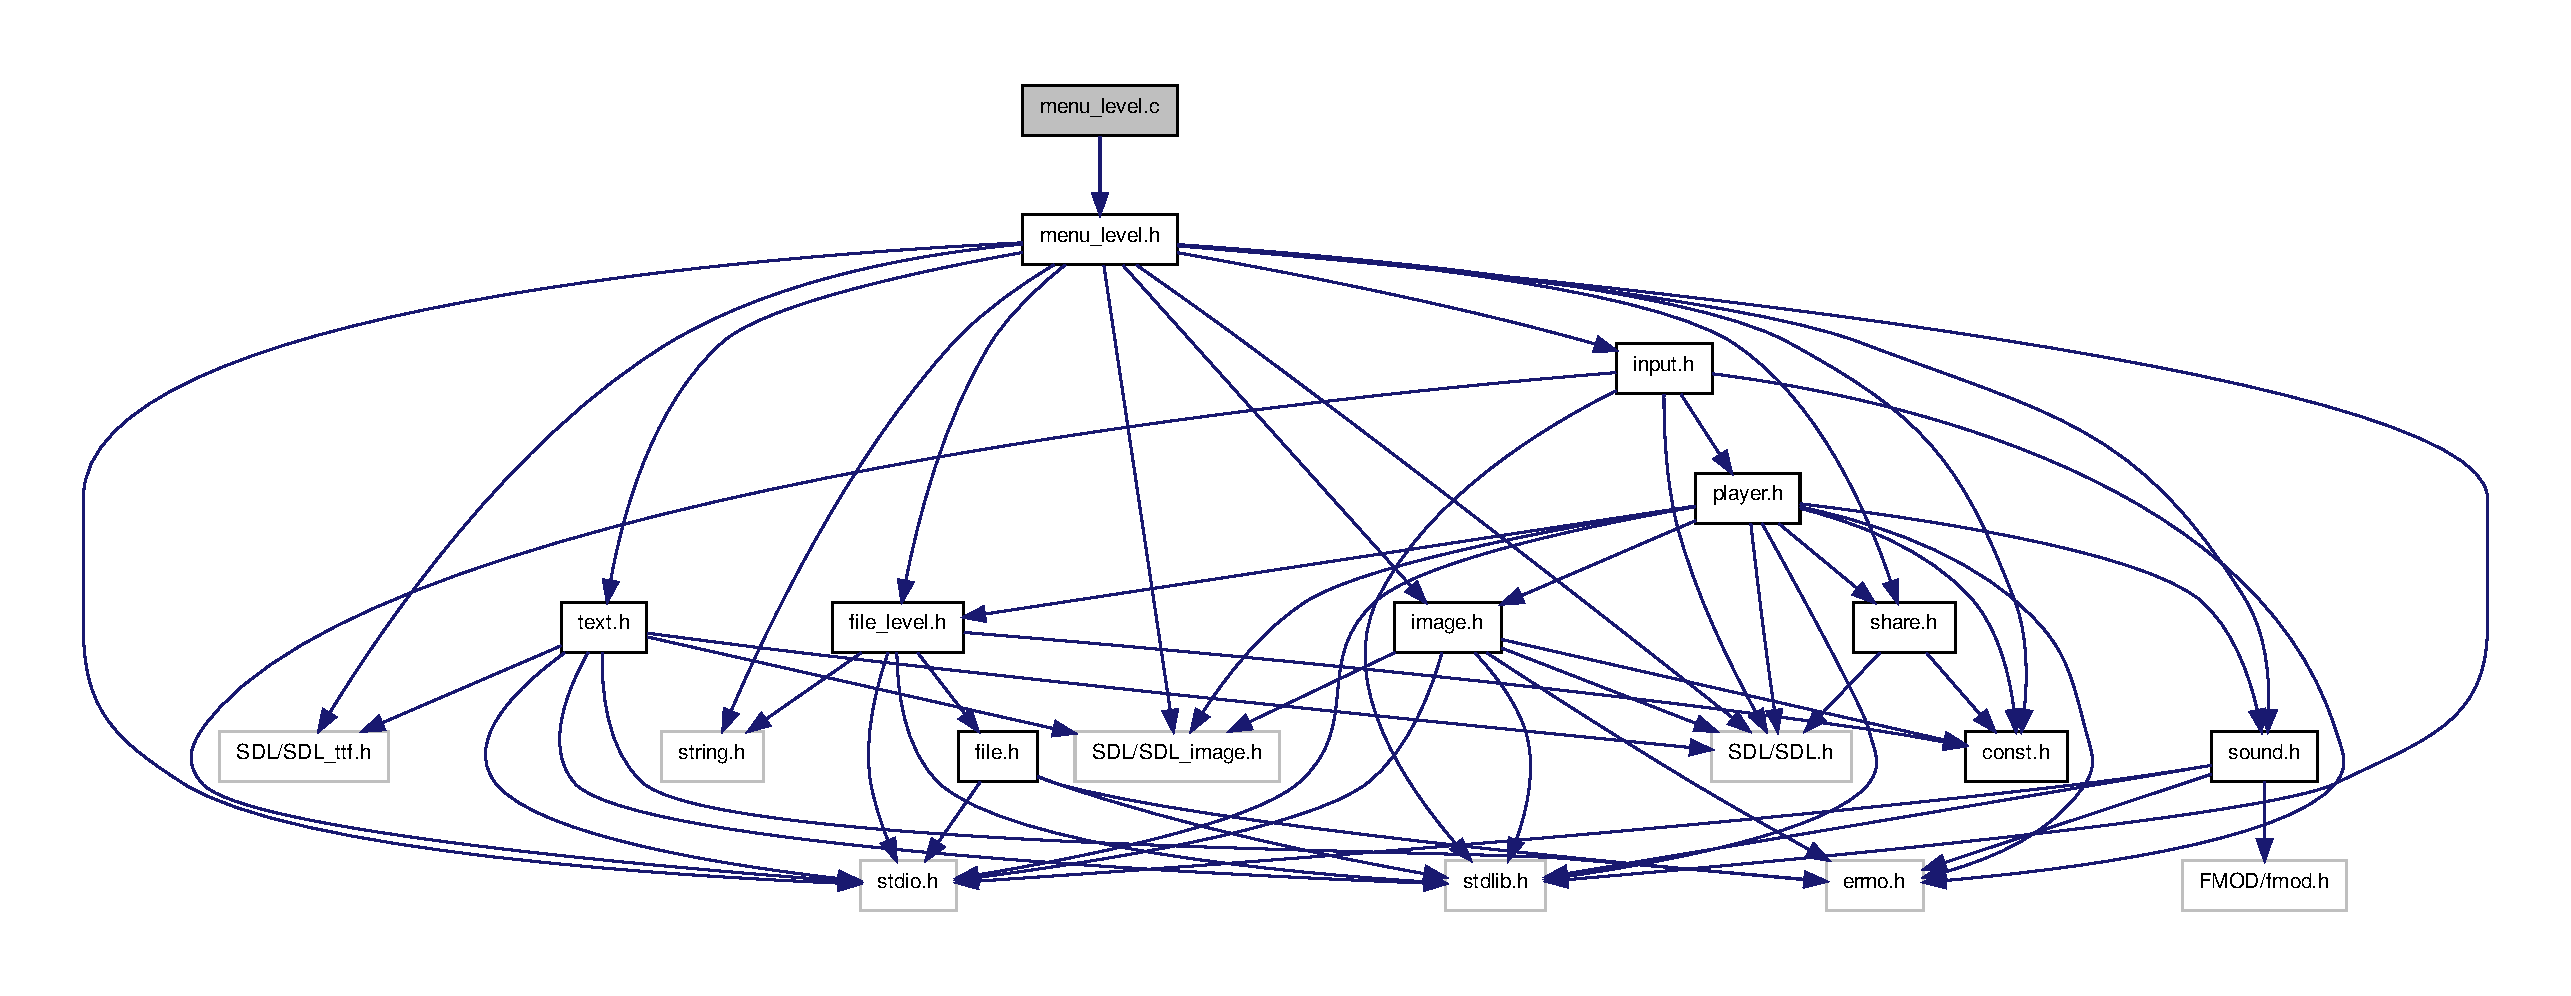
\includegraphics[width=350pt]{menu__level_8c__incl}
\end{center}
\end{figure}
\subsection*{Functions}
\begin{DoxyCompactItemize}
\item 
\hypertarget{menu__level_8c_a794ae7f9d9b9deb8594ec894ef18a2de}{int {\bfseries menu\-Level} (S\-D\-L\-\_\-\-Surface $\ast$screen, char level\-\_\-name\mbox{[}M\-A\-X\-\_\-\-S\-I\-Z\-E\-\_\-\-F\-I\-L\-E\-\_\-\-N\-A\-M\-E\mbox{]}, \hyperlink{struct_sound}{Sound} $\ast$sound\-\_\-sys, char player\-\_\-name\mbox{[}M\-A\-X\-\_\-\-S\-I\-Z\-E\-\_\-\-F\-I\-L\-E\-\_\-\-N\-A\-M\-E\mbox{]}, \hyperlink{struct_player}{Player} $\ast$player, int $\ast$go, int $\ast$nb\-\_\-lvl, \hyperlink{struct_input}{Input} $\ast$in)}\label{menu__level_8c_a794ae7f9d9b9deb8594ec894ef18a2de}

\end{DoxyCompactItemize}


\subsection{Detailed Description}
level choose menu \begin{DoxyAuthor}{Author}
Remi B\-E\-R\-T\-H\-O 
\end{DoxyAuthor}
\begin{DoxyDate}{Date}
15/03/14 
\end{DoxyDate}

\hypertarget{menu__level_8h}{\section{menu\-\_\-level.\-h File Reference}
\label{menu__level_8h}\index{menu\-\_\-level.\-h@{menu\-\_\-level.\-h}}
}


Menu gerant le choix du niveau.  


{\ttfamily \#include $<$stdio.\-h$>$}\\*
{\ttfamily \#include $<$stdlib.\-h$>$}\\*
{\ttfamily \#include $<$string.\-h$>$}\\*
{\ttfamily \#include $<$S\-D\-L/\-S\-D\-L.\-h$>$}\\*
{\ttfamily \#include $<$S\-D\-L/\-S\-D\-L\-\_\-image.\-h$>$}\\*
{\ttfamily \#include $<$S\-D\-L/\-S\-D\-L\-\_\-ttf.\-h$>$}\\*
{\ttfamily \#include \char`\"{}const.\-h\char`\"{}}\\*
{\ttfamily \#include \char`\"{}file\-\_\-level.\-h\char`\"{}}\\*
{\ttfamily \#include \char`\"{}share.\-h\char`\"{}}\\*
{\ttfamily \#include \char`\"{}text.\-h\char`\"{}}\\*
{\ttfamily \#include \char`\"{}sound.\-h\char`\"{}}\\*
Include dependency graph for menu\-\_\-level.\-h\-:
\nopagebreak
\begin{figure}[H]
\begin{center}
\leavevmode
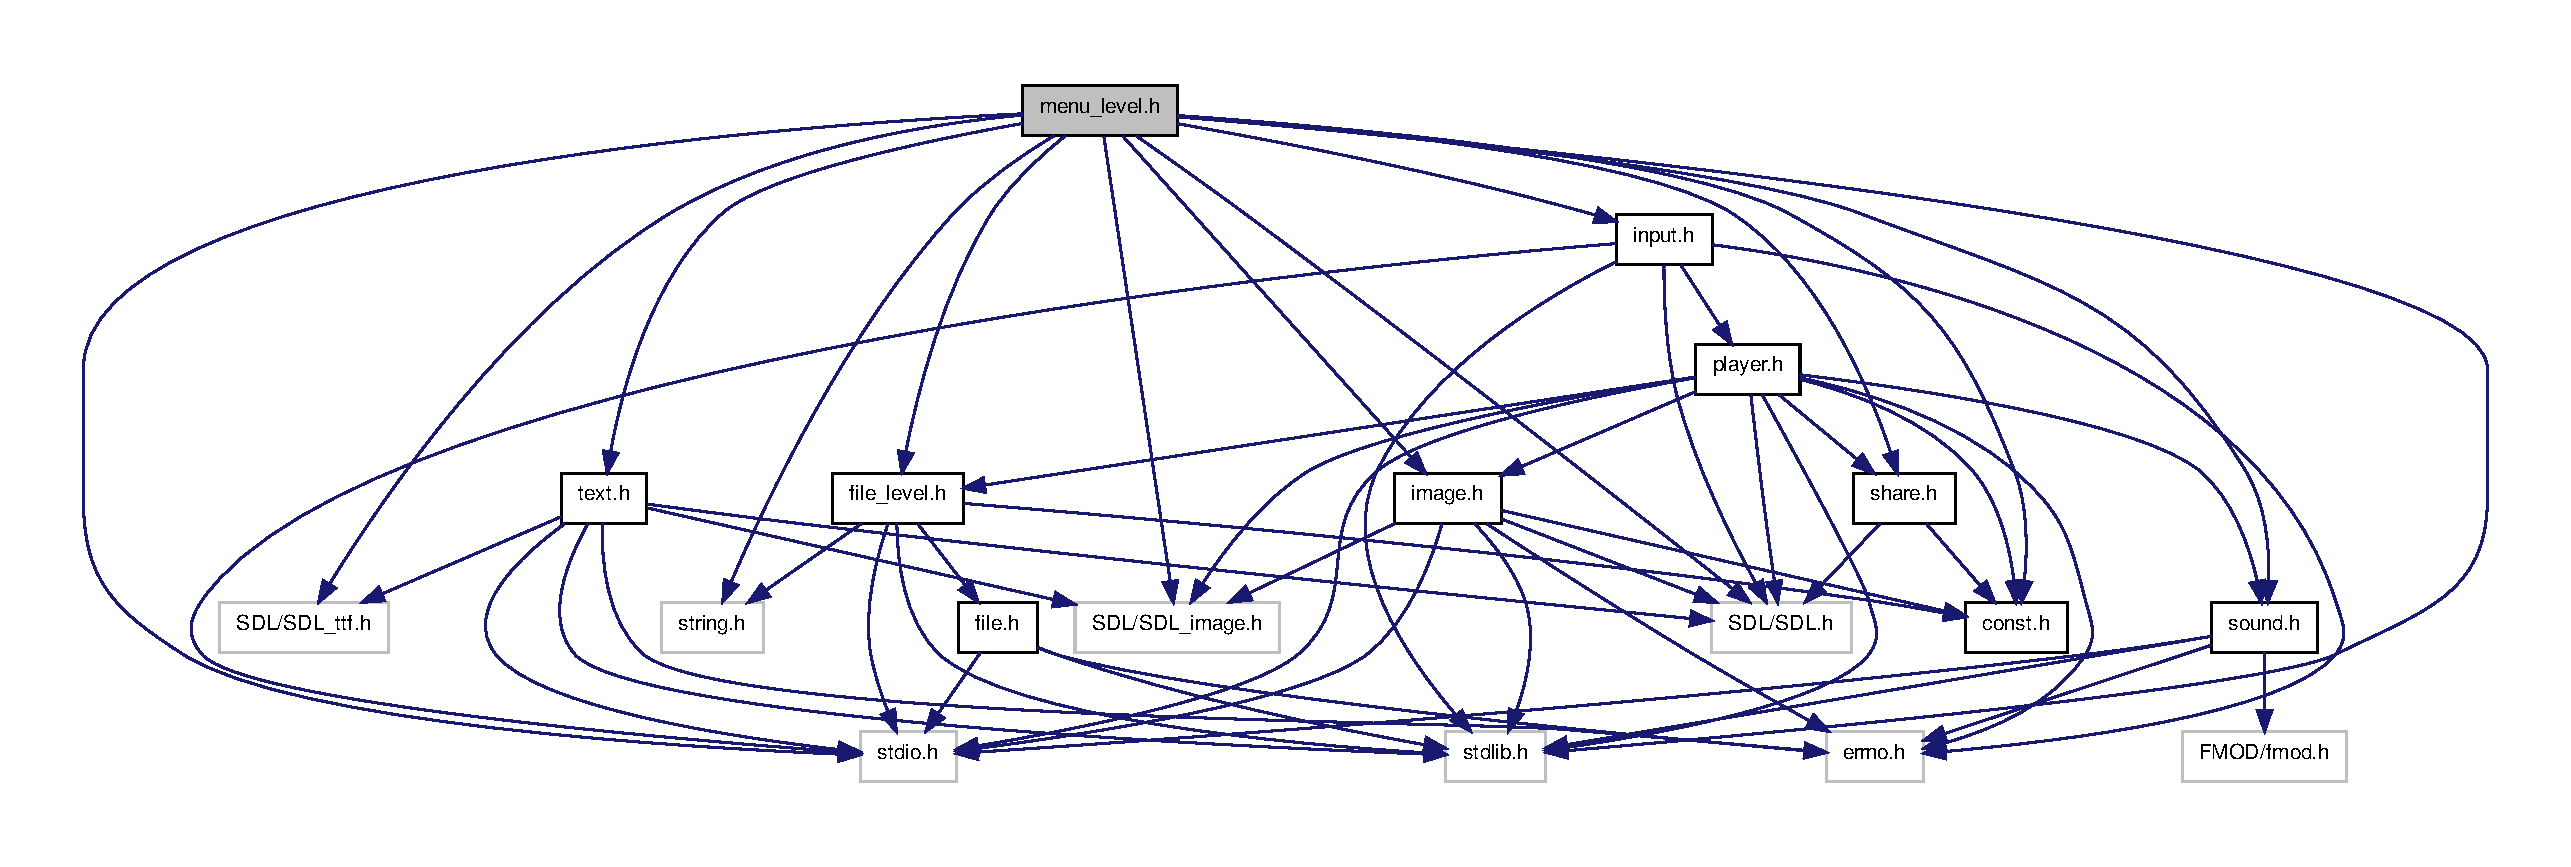
\includegraphics[width=350pt]{menu__level_8h__incl}
\end{center}
\end{figure}
This graph shows which files directly or indirectly include this file\-:
\nopagebreak
\begin{figure}[H]
\begin{center}
\leavevmode
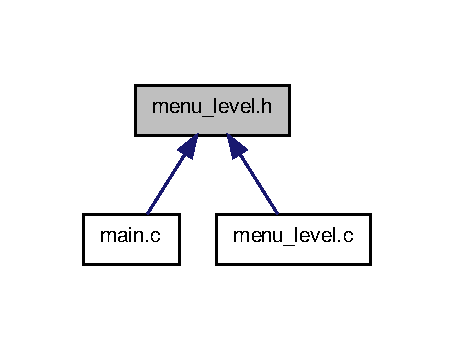
\includegraphics[width=154pt]{menu__level_8h__dep__incl}
\end{center}
\end{figure}
\subsection*{Functions}
\begin{DoxyCompactItemize}
\item 
\hypertarget{menu__level_8h_a2df6ef1e00c1fe9c46d267b8f0f56adf}{int {\bfseries menu\-Level} (S\-D\-L\-\_\-\-Surface $\ast$screen, char level\-\_\-name\mbox{[}T\-A\-I\-L\-L\-E\-\_\-\-M\-A\-X\-\_\-\-N\-O\-M\-\_\-\-F\-I\-C\-H\-I\-E\-R\mbox{]}, \hyperlink{struct_sound}{Sound} $\ast$s)}\label{menu__level_8h_a2df6ef1e00c1fe9c46d267b8f0f56adf}

\end{DoxyCompactItemize}


\subsection{Detailed Description}
Menu gerant le choix du niveau. \begin{DoxyAuthor}{Author}
Remi B\-E\-R\-T\-H\-O 
\end{DoxyAuthor}
\begin{DoxyDate}{Date}
15/03/14 
\end{DoxyDate}
\begin{DoxyVersion}{Version}
1.\-0 
\end{DoxyVersion}

\hypertarget{menu__option_8c}{\subsection{menu\-\_\-option.\-c File Reference}
\label{menu__option_8c}\index{menu\-\_\-option.\-c@{menu\-\_\-option.\-c}}
}


contain the option menu functions  


{\ttfamily \#include \char`\"{}menu\-\_\-option.\-h\char`\"{}}\\*
\subsubsection*{Functions}
\begin{DoxyCompactItemize}
\item 
int \hyperlink{menu__option_8c_a3529f1d52146bafa1f04dcf740ee0056}{menu\-Options} (S\-D\-L\-\_\-\-Surface $\ast$screen, int $\ast$go, S\-D\-L\-Key $\ast$kc)
\item 
void \hyperlink{menu__option_8c_aec745341a7cdd39be0329420a1dccc43}{key\-Board\-Options} (S\-D\-L\-\_\-\-Surface $\ast$screen, int $\ast$go, S\-D\-L\-Key $\ast$kc)
\item 
void \hyperlink{menu__option_8c_a09208fc21970afd80a59971051150a3b}{choose\-Key} (S\-D\-L\-\_\-\-Surface $\ast$screen, \hyperlink{struct_input}{Input} $\ast$in, char $\ast$action, S\-D\-L\-Key $\ast$kc, int nb)
\end{DoxyCompactItemize}


\subsubsection{Detailed Description}
contain the option menu functions \begin{DoxyAuthor}{Author}
Xavier C\-O\-P\-O\-N\-E\-T 
\end{DoxyAuthor}
\begin{DoxyDate}{Date}
2014-\/04-\/27 
\end{DoxyDate}


\subsubsection{Function Documentation}
\hypertarget{menu__option_8c_a09208fc21970afd80a59971051150a3b}{\index{menu\-\_\-option.\-c@{menu\-\_\-option.\-c}!choose\-Key@{choose\-Key}}
\index{choose\-Key@{choose\-Key}!menu_option.c@{menu\-\_\-option.\-c}}
\paragraph[{choose\-Key}]{\setlength{\rightskip}{0pt plus 5cm}void choose\-Key (
\begin{DoxyParamCaption}
\item[{S\-D\-L\-\_\-\-Surface $\ast$}]{screen, }
\item[{{\bf Input} $\ast$}]{in, }
\item[{char $\ast$}]{action, }
\item[{S\-D\-L\-Key $\ast$}]{kc, }
\item[{int}]{nb}
\end{DoxyParamCaption}
)}}\label{menu__option_8c_a09208fc21970afd80a59971051150a3b}
print the message asking the player to choose a key and wait until the player press a key and deals with this key 
\begin{DoxyParams}[1]{Parameters}
\mbox{\tt out}  & {\em screen} & the game screen \\
\hline
\mbox{\tt in,out}  & {\em in} & the input structure \\
\hline
\mbox{\tt in}  & {\em action} & the action which the key has to be choosen \\
\hline
\mbox{\tt out}  & {\em kc} & the keyboard configuration \\
\hline
\mbox{\tt in}  & {\em nb} & the number of the action \\
\hline
\end{DoxyParams}


Here is the call graph for this function\-:\nopagebreak
\begin{figure}[H]
\begin{center}
\leavevmode
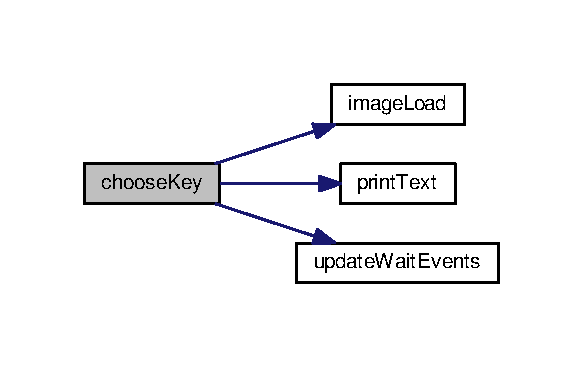
\includegraphics[width=280pt]{menu__option_8c_a09208fc21970afd80a59971051150a3b_cgraph}
\end{center}
\end{figure}


\hypertarget{menu__option_8c_aec745341a7cdd39be0329420a1dccc43}{\index{menu\-\_\-option.\-c@{menu\-\_\-option.\-c}!key\-Board\-Options@{key\-Board\-Options}}
\index{key\-Board\-Options@{key\-Board\-Options}!menu_option.c@{menu\-\_\-option.\-c}}
\paragraph[{key\-Board\-Options}]{\setlength{\rightskip}{0pt plus 5cm}void key\-Board\-Options (
\begin{DoxyParamCaption}
\item[{S\-D\-L\-\_\-\-Surface $\ast$}]{screen, }
\item[{int $\ast$}]{go, }
\item[{S\-D\-L\-Key $\ast$}]{kc}
\end{DoxyParamCaption}
)}}\label{menu__option_8c_aec745341a7cdd39be0329420a1dccc43}
print the keyboard options and deals with the user choises 
\begin{DoxyParams}[1]{Parameters}
\mbox{\tt out}  & {\em screen} & the game screen \\
\hline
\mbox{\tt in,out}  & {\em go} & main loop validation \\
\hline
\mbox{\tt in,out}  & {\em kc} & the keyboard config \\
\hline
\end{DoxyParams}


Here is the call graph for this function\-:\nopagebreak
\begin{figure}[H]
\begin{center}
\leavevmode
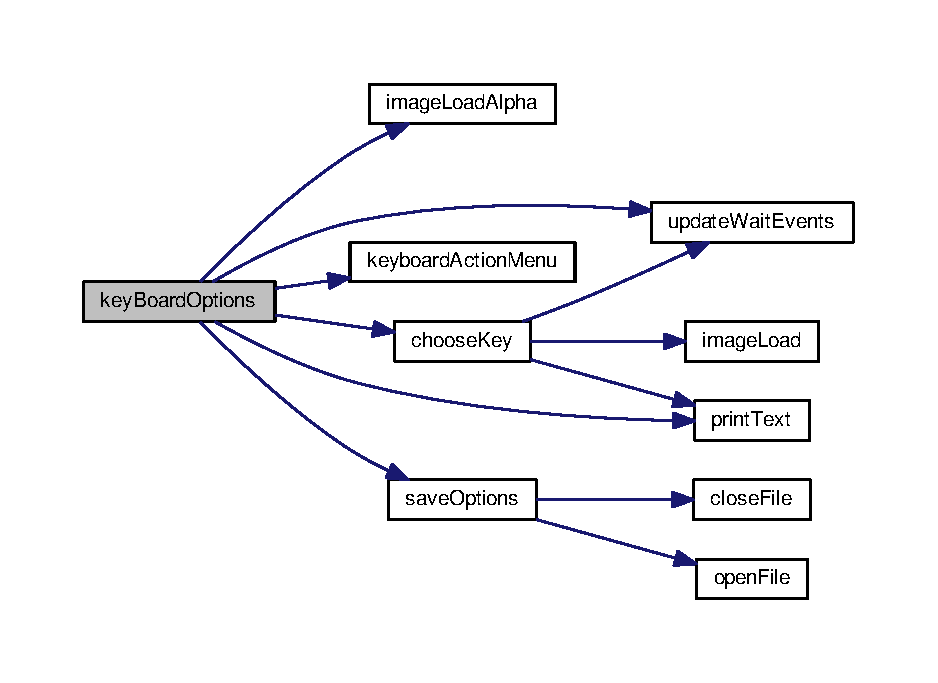
\includegraphics[width=350pt]{menu__option_8c_aec745341a7cdd39be0329420a1dccc43_cgraph}
\end{center}
\end{figure}


\hypertarget{menu__option_8c_a3529f1d52146bafa1f04dcf740ee0056}{\index{menu\-\_\-option.\-c@{menu\-\_\-option.\-c}!menu\-Options@{menu\-Options}}
\index{menu\-Options@{menu\-Options}!menu_option.c@{menu\-\_\-option.\-c}}
\paragraph[{menu\-Options}]{\setlength{\rightskip}{0pt plus 5cm}int menu\-Options (
\begin{DoxyParamCaption}
\item[{S\-D\-L\-\_\-\-Surface $\ast$}]{screen, }
\item[{int $\ast$}]{go, }
\item[{S\-D\-L\-Key $\ast$}]{kc}
\end{DoxyParamCaption}
)}}\label{menu__option_8c_a3529f1d52146bafa1f04dcf740ee0056}
print the option menu on the screen 
\begin{DoxyParams}[1]{Parameters}
\mbox{\tt out}  & {\em screen} & the game screen \\
\hline
\mbox{\tt in,out}  & {\em go} & main loop validation \\
\hline
\mbox{\tt in,out}  & {\em kc} & the keyboard configuration \\
\hline
\end{DoxyParams}
\begin{DoxyReturn}{Returns}
the number of the option which is choosen, -\/1 if esc 
\end{DoxyReturn}


Here is the call graph for this function\-:\nopagebreak
\begin{figure}[H]
\begin{center}
\leavevmode
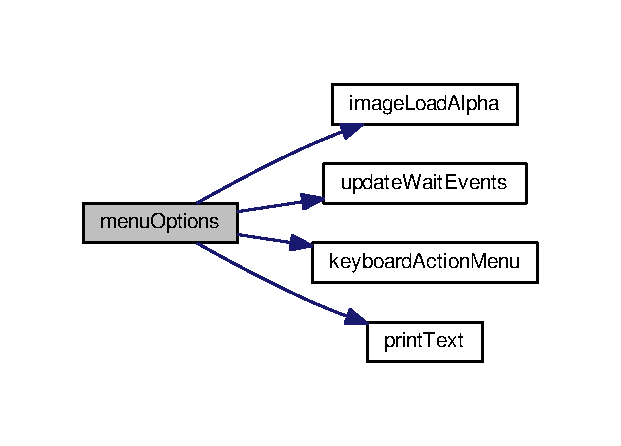
\includegraphics[width=298pt]{menu__option_8c_a3529f1d52146bafa1f04dcf740ee0056_cgraph}
\end{center}
\end{figure}



\hypertarget{menu__option_8h}{\subsection{menu\-\_\-option.\-h File Reference}
\label{menu__option_8h}\index{menu\-\_\-option.\-h@{menu\-\_\-option.\-h}}
}


\hyperlink{menu__option_8c}{menu\-\_\-option.\-c} header  


{\ttfamily \#include $<$stdlib.\-h$>$}\\*
{\ttfamily \#include $<$stdio.\-h$>$}\\*
{\ttfamily \#include $<$errno.\-h$>$}\\*
{\ttfamily \#include $<$S\-D\-L/\-S\-D\-L.\-h$>$}\\*
{\ttfamily \#include $<$S\-D\-L/\-S\-D\-L\-\_\-image.\-h$>$}\\*
{\ttfamily \#include $<$S\-D\-L/\-S\-D\-L\-\_\-ttf.\-h$>$}\\*
{\ttfamily \#include \char`\"{}const.\-h\char`\"{}}\\*
{\ttfamily \#include \char`\"{}text.\-h\char`\"{}}\\*
{\ttfamily \#include \char`\"{}share.\-h\char`\"{}}\\*
{\ttfamily \#include \char`\"{}image.\-h\char`\"{}}\\*
{\ttfamily \#include \char`\"{}input.\-h\char`\"{}}\\*
{\ttfamily \#include \char`\"{}option.\-h\char`\"{}}\\*
\subsubsection*{Functions}
\begin{DoxyCompactItemize}
\item 
int \hyperlink{menu__option_8h_a3529f1d52146bafa1f04dcf740ee0056}{menu\-Options} (S\-D\-L\-\_\-\-Surface $\ast$screen, int $\ast$go, S\-D\-L\-Key $\ast$kc)
\item 
void \hyperlink{menu__option_8h_aec745341a7cdd39be0329420a1dccc43}{key\-Board\-Options} (S\-D\-L\-\_\-\-Surface $\ast$screen, int $\ast$go, S\-D\-L\-Key $\ast$kc)
\item 
void \hyperlink{menu__option_8h_a09208fc21970afd80a59971051150a3b}{choose\-Key} (S\-D\-L\-\_\-\-Surface $\ast$screen, \hyperlink{struct_input}{Input} $\ast$in, char $\ast$action, S\-D\-L\-Key $\ast$kc, int nb)
\end{DoxyCompactItemize}


\subsubsection{Detailed Description}
\hyperlink{menu__option_8c}{menu\-\_\-option.\-c} header \begin{DoxyAuthor}{Author}
Xavier C\-O\-P\-O\-N\-E\-T 
\end{DoxyAuthor}
\begin{DoxyDate}{Date}
2014-\/04-\/27 
\end{DoxyDate}


\subsubsection{Function Documentation}
\hypertarget{menu__option_8h_a09208fc21970afd80a59971051150a3b}{\index{menu\-\_\-option.\-h@{menu\-\_\-option.\-h}!choose\-Key@{choose\-Key}}
\index{choose\-Key@{choose\-Key}!menu_option.h@{menu\-\_\-option.\-h}}
\paragraph[{choose\-Key}]{\setlength{\rightskip}{0pt plus 5cm}void choose\-Key (
\begin{DoxyParamCaption}
\item[{S\-D\-L\-\_\-\-Surface $\ast$}]{screen, }
\item[{{\bf Input} $\ast$}]{in, }
\item[{char $\ast$}]{action, }
\item[{S\-D\-L\-Key $\ast$}]{kc, }
\item[{int}]{nb}
\end{DoxyParamCaption}
)}}\label{menu__option_8h_a09208fc21970afd80a59971051150a3b}
print the message asking the player to choose a key and wait until the player press a key and deals with this key 
\begin{DoxyParams}[1]{Parameters}
\mbox{\tt out}  & {\em screen} & the game screen \\
\hline
\mbox{\tt in,out}  & {\em in} & the input structure \\
\hline
\mbox{\tt in}  & {\em action} & the action which the key has to be choosen \\
\hline
\mbox{\tt out}  & {\em kc} & the keyboard configuration \\
\hline
\mbox{\tt in}  & {\em nb} & the number of the action \\
\hline
\end{DoxyParams}


Here is the call graph for this function\-:
\nopagebreak
\begin{figure}[H]
\begin{center}
\leavevmode
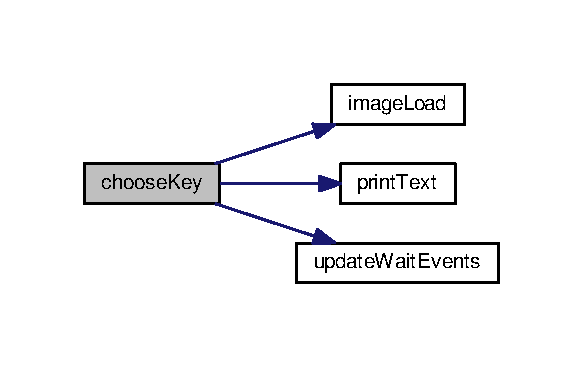
\includegraphics[width=280pt]{menu__option_8h_a09208fc21970afd80a59971051150a3b_cgraph}
\end{center}
\end{figure}


\hypertarget{menu__option_8h_aec745341a7cdd39be0329420a1dccc43}{\index{menu\-\_\-option.\-h@{menu\-\_\-option.\-h}!key\-Board\-Options@{key\-Board\-Options}}
\index{key\-Board\-Options@{key\-Board\-Options}!menu_option.h@{menu\-\_\-option.\-h}}
\paragraph[{key\-Board\-Options}]{\setlength{\rightskip}{0pt plus 5cm}void key\-Board\-Options (
\begin{DoxyParamCaption}
\item[{S\-D\-L\-\_\-\-Surface $\ast$}]{screen, }
\item[{int $\ast$}]{go, }
\item[{S\-D\-L\-Key $\ast$}]{kc}
\end{DoxyParamCaption}
)}}\label{menu__option_8h_aec745341a7cdd39be0329420a1dccc43}
print the keyboard options and deals with the user choises 
\begin{DoxyParams}[1]{Parameters}
\mbox{\tt out}  & {\em screen} & the game screen \\
\hline
\mbox{\tt in,out}  & {\em go} & main loop validation \\
\hline
\mbox{\tt in,out}  & {\em kc} & the keyboard config \\
\hline
\end{DoxyParams}


Here is the call graph for this function\-:
\nopagebreak
\begin{figure}[H]
\begin{center}
\leavevmode
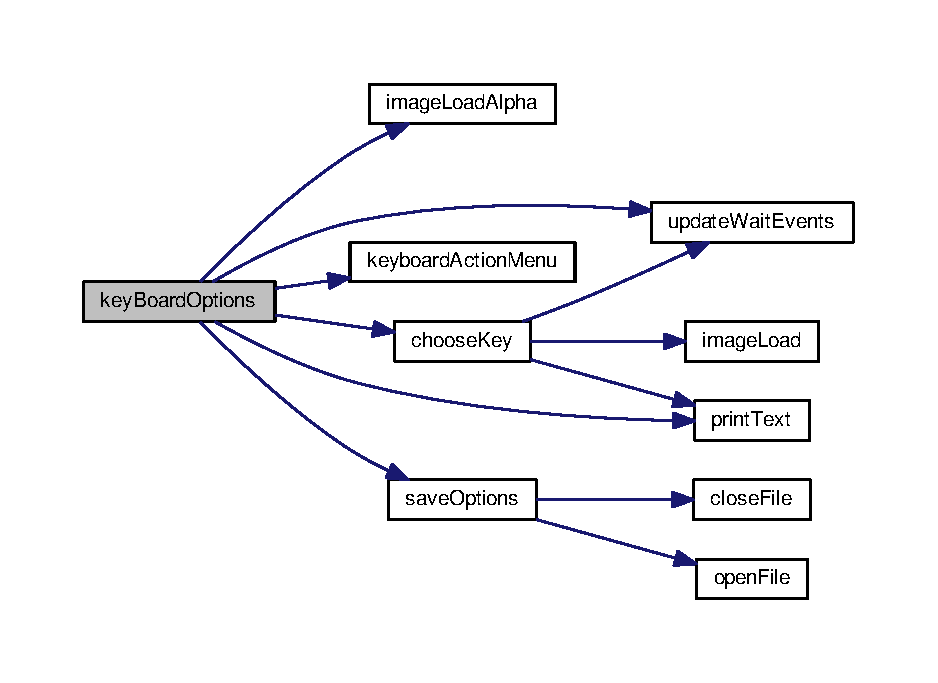
\includegraphics[width=350pt]{menu__option_8h_aec745341a7cdd39be0329420a1dccc43_cgraph}
\end{center}
\end{figure}


\hypertarget{menu__option_8h_a3529f1d52146bafa1f04dcf740ee0056}{\index{menu\-\_\-option.\-h@{menu\-\_\-option.\-h}!menu\-Options@{menu\-Options}}
\index{menu\-Options@{menu\-Options}!menu_option.h@{menu\-\_\-option.\-h}}
\paragraph[{menu\-Options}]{\setlength{\rightskip}{0pt plus 5cm}int menu\-Options (
\begin{DoxyParamCaption}
\item[{S\-D\-L\-\_\-\-Surface $\ast$}]{screen, }
\item[{int $\ast$}]{go, }
\item[{S\-D\-L\-Key $\ast$}]{kc}
\end{DoxyParamCaption}
)}}\label{menu__option_8h_a3529f1d52146bafa1f04dcf740ee0056}
print the option menu on the screen 
\begin{DoxyParams}[1]{Parameters}
\mbox{\tt out}  & {\em screen} & the game screen \\
\hline
\mbox{\tt in,out}  & {\em go} & main loop validation \\
\hline
\mbox{\tt in,out}  & {\em kc} & the keyboard configuration \\
\hline
\end{DoxyParams}
\begin{DoxyReturn}{Returns}
the number of the option which is choosen, -\/1 if esc 
\end{DoxyReturn}


Here is the call graph for this function\-:
\nopagebreak
\begin{figure}[H]
\begin{center}
\leavevmode
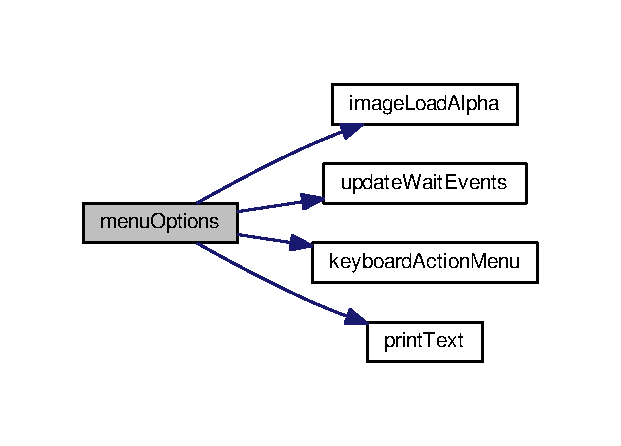
\includegraphics[width=298pt]{menu__option_8h_a3529f1d52146bafa1f04dcf740ee0056_cgraph}
\end{center}
\end{figure}



\hypertarget{option_8c}{\subsection{option.\-c File Reference}
\label{option_8c}\index{option.\-c@{option.\-c}}
}


contains the funtions that manipulate the options  


{\ttfamily \#include \char`\"{}option.\-h\char`\"{}}\\*
\subsubsection*{Functions}
\begin{DoxyCompactItemize}
\item 
void \hyperlink{option_8c_a82de9e33ffe49578aedcb1796c2a524c}{load\-Sound\-Options} (char conf\-File\mbox{[}$\,$\mbox{]}, \hyperlink{struct_sound}{Sound} $\ast$sound\-Sys)
\item 
void \hyperlink{option_8c_ab75794ec6a13d9a1538d9f4fa2cb60f0}{save\-Sound\-Options} (char conf\-File\mbox{[}$\,$\mbox{]}, \hyperlink{struct_sound}{Sound} $\ast$sound\-Sys)
\item 
void \hyperlink{option_8c_a7f505e8b70cf0674aac99379c7b0a3ce}{load\-Input\-Options} (char player\-\_\-name\mbox{[}$\,$\mbox{]}, S\-D\-L\-Key $\ast$kc, \hyperlink{struct_input}{Input} $\ast$in)
\item 
void \hyperlink{option_8c_a8c9263c45096babd087bb2b1eafa0859}{save\-Input\-Options} (char player\-\_\-name\mbox{[}$\,$\mbox{]}, S\-D\-L\-Key $\ast$kc, \hyperlink{struct_input}{Input} $\ast$in)
\end{DoxyCompactItemize}


\subsubsection{Detailed Description}
contains the funtions that manipulate the options \begin{DoxyAuthor}{Author}
X.\-C\-O\-P\-O\-N\-E\-T 
\end{DoxyAuthor}
\begin{DoxyDate}{Date}
2014-\/04-\/28 
\end{DoxyDate}


\subsubsection{Function Documentation}
\hypertarget{option_8c_a7f505e8b70cf0674aac99379c7b0a3ce}{\index{option.\-c@{option.\-c}!load\-Input\-Options@{load\-Input\-Options}}
\index{load\-Input\-Options@{load\-Input\-Options}!option.c@{option.\-c}}
\paragraph[{load\-Input\-Options}]{\setlength{\rightskip}{0pt plus 5cm}void load\-Input\-Options (
\begin{DoxyParamCaption}
\item[{char}]{player\-\_\-name\mbox{[}$\,$\mbox{]}, }
\item[{S\-D\-L\-Key $\ast$}]{kc, }
\item[{{\bf Input} $\ast$}]{in}
\end{DoxyParamCaption}
)}}\label{option_8c_a7f505e8b70cf0674aac99379c7b0a3ce}
load the input options from the player input config file 
\begin{DoxyParams}[1]{Parameters}
\mbox{\tt in}  & {\em player\-\_\-name} & the current player's name \\
\hline
\mbox{\tt out}  & {\em kc} & the keyboard configuration structure \\
\hline
\mbox{\tt out}  & {\em in} & the input structure \\
\hline
\end{DoxyParams}


Here is the call graph for this function\-:
\nopagebreak
\begin{figure}[H]
\begin{center}
\leavevmode
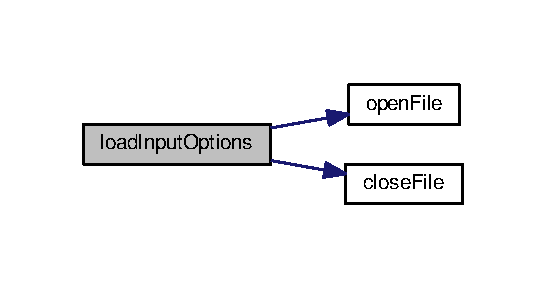
\includegraphics[width=262pt]{option_8c_a7f505e8b70cf0674aac99379c7b0a3ce_cgraph}
\end{center}
\end{figure}


\hypertarget{option_8c_a82de9e33ffe49578aedcb1796c2a524c}{\index{option.\-c@{option.\-c}!load\-Sound\-Options@{load\-Sound\-Options}}
\index{load\-Sound\-Options@{load\-Sound\-Options}!option.c@{option.\-c}}
\paragraph[{load\-Sound\-Options}]{\setlength{\rightskip}{0pt plus 5cm}void load\-Sound\-Options (
\begin{DoxyParamCaption}
\item[{char}]{conf\-File\mbox{[}$\,$\mbox{]}, }
\item[{{\bf Sound} $\ast$}]{sound\-Sys}
\end{DoxyParamCaption}
)}}\label{option_8c_a82de9e33ffe49578aedcb1796c2a524c}
load the sound options from the sound config file 
\begin{DoxyParams}[1]{Parameters}
\mbox{\tt in}  & {\em conf\-File} & the config file path \\
\hline
\mbox{\tt out}  & {\em sound\-Sys} & the sound system \\
\hline
\end{DoxyParams}


Here is the call graph for this function\-:
\nopagebreak
\begin{figure}[H]
\begin{center}
\leavevmode
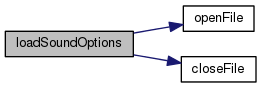
\includegraphics[width=268pt]{option_8c_a82de9e33ffe49578aedcb1796c2a524c_cgraph}
\end{center}
\end{figure}


\hypertarget{option_8c_a8c9263c45096babd087bb2b1eafa0859}{\index{option.\-c@{option.\-c}!save\-Input\-Options@{save\-Input\-Options}}
\index{save\-Input\-Options@{save\-Input\-Options}!option.c@{option.\-c}}
\paragraph[{save\-Input\-Options}]{\setlength{\rightskip}{0pt plus 5cm}void save\-Input\-Options (
\begin{DoxyParamCaption}
\item[{char}]{player\-\_\-name\mbox{[}$\,$\mbox{]}, }
\item[{S\-D\-L\-Key $\ast$}]{kc, }
\item[{{\bf Input} $\ast$}]{in}
\end{DoxyParamCaption}
)}}\label{option_8c_a8c9263c45096babd087bb2b1eafa0859}
save the input options to the player input config file 
\begin{DoxyParams}[1]{Parameters}
\mbox{\tt in}  & {\em player\-\_\-name} & the current player name \\
\hline
\mbox{\tt out}  & {\em kc} & the keyboard configuration structure \\
\hline
\mbox{\tt out}  & {\em in} & the input structure \\
\hline
\end{DoxyParams}


Here is the call graph for this function\-:
\nopagebreak
\begin{figure}[H]
\begin{center}
\leavevmode
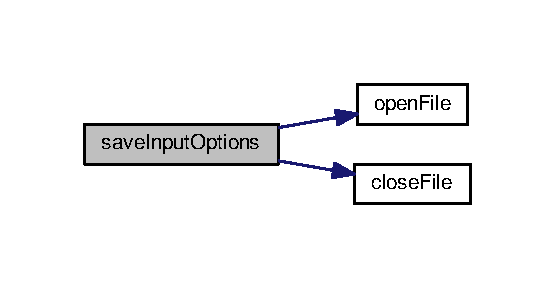
\includegraphics[width=266pt]{option_8c_a8c9263c45096babd087bb2b1eafa0859_cgraph}
\end{center}
\end{figure}


\hypertarget{option_8c_ab75794ec6a13d9a1538d9f4fa2cb60f0}{\index{option.\-c@{option.\-c}!save\-Sound\-Options@{save\-Sound\-Options}}
\index{save\-Sound\-Options@{save\-Sound\-Options}!option.c@{option.\-c}}
\paragraph[{save\-Sound\-Options}]{\setlength{\rightskip}{0pt plus 5cm}void save\-Sound\-Options (
\begin{DoxyParamCaption}
\item[{char}]{conf\-File\mbox{[}$\,$\mbox{]}, }
\item[{{\bf Sound} $\ast$}]{sound\-Sys}
\end{DoxyParamCaption}
)}}\label{option_8c_ab75794ec6a13d9a1538d9f4fa2cb60f0}
save the sound options to the config file 
\begin{DoxyParams}[1]{Parameters}
\mbox{\tt in}  & {\em conf\-File} & the config file path \\
\hline
\mbox{\tt in}  & {\em sound\-Sys} & the sound system \\
\hline
\end{DoxyParams}


Here is the call graph for this function\-:
\nopagebreak
\begin{figure}[H]
\begin{center}
\leavevmode
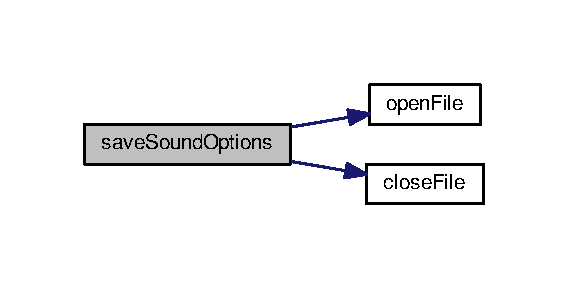
\includegraphics[width=272pt]{option_8c_ab75794ec6a13d9a1538d9f4fa2cb60f0_cgraph}
\end{center}
\end{figure}



\hypertarget{option_8h}{\subsection{option.\-h File Reference}
\label{option_8h}\index{option.\-h@{option.\-h}}
}


\hyperlink{option_8c}{option.\-c} header  


{\ttfamily \#include \char`\"{}file.\-h\char`\"{}}\\*
{\ttfamily \#include \char`\"{}structures.\-h\char`\"{}}\\*
{\ttfamily \#include \char`\"{}input.\-h\char`\"{}}\\*
\subsubsection*{Functions}
\begin{DoxyCompactItemize}
\item 
void \hyperlink{option_8h_ae25f1e88b32a9246a4b222b9210fefb8}{load\-Options} (char conf\-File\mbox{[}$\,$\mbox{]}, S\-D\-L\-Key $\ast$kc)
\item 
void \hyperlink{option_8h_aa47c7d9be8978d36b12c582b701c534d}{save\-Options} (char conf\-File\mbox{[}$\,$\mbox{]}, S\-D\-L\-Key $\ast$kc)
\end{DoxyCompactItemize}


\subsubsection{Detailed Description}
\hyperlink{option_8c}{option.\-c} header \begin{DoxyAuthor}{Author}
Xavier C\-O\-P\-O\-N\-E\-T 
\end{DoxyAuthor}
\begin{DoxyDate}{Date}
2014-\/04-\/28 
\end{DoxyDate}


\subsubsection{Function Documentation}
\hypertarget{option_8h_ae25f1e88b32a9246a4b222b9210fefb8}{\index{option.\-h@{option.\-h}!load\-Options@{load\-Options}}
\index{load\-Options@{load\-Options}!option.h@{option.\-h}}
\paragraph[{load\-Options}]{\setlength{\rightskip}{0pt plus 5cm}void load\-Options (
\begin{DoxyParamCaption}
\item[{char}]{conf\-File\mbox{[}$\,$\mbox{]}, }
\item[{S\-D\-L\-Key $\ast$}]{kc}
\end{DoxyParamCaption}
)}}\label{option_8h_ae25f1e88b32a9246a4b222b9210fefb8}
Load the options from the config file 
\begin{DoxyParams}[1]{Parameters}
\mbox{\tt in}  & {\em conf\-File} & the config file path \\
\hline
\mbox{\tt out}  & {\em kc} & the keyboard configuration structure \\
\hline
\end{DoxyParams}


Here is the call graph for this function\-:
\nopagebreak
\begin{figure}[H]
\begin{center}
\leavevmode
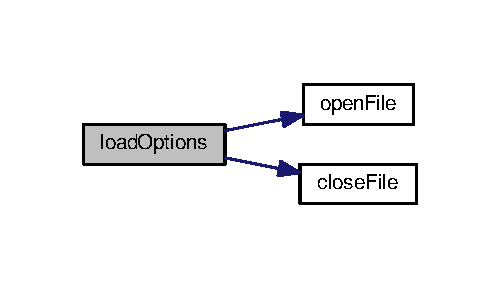
\includegraphics[width=240pt]{option_8h_ae25f1e88b32a9246a4b222b9210fefb8_cgraph}
\end{center}
\end{figure}


\hypertarget{option_8h_aa47c7d9be8978d36b12c582b701c534d}{\index{option.\-h@{option.\-h}!save\-Options@{save\-Options}}
\index{save\-Options@{save\-Options}!option.h@{option.\-h}}
\paragraph[{save\-Options}]{\setlength{\rightskip}{0pt plus 5cm}void save\-Options (
\begin{DoxyParamCaption}
\item[{char}]{conf\-File\mbox{[}$\,$\mbox{]}, }
\item[{S\-D\-L\-Key $\ast$}]{kc}
\end{DoxyParamCaption}
)}}\label{option_8h_aa47c7d9be8978d36b12c582b701c534d}
save the options to the config file 
\begin{DoxyParams}[1]{Parameters}
\mbox{\tt in}  & {\em conf\-File} & the config file path \\
\hline
\mbox{\tt in}  & {\em kc} & the keyboard configuration structure \\
\hline
\end{DoxyParams}


Here is the call graph for this function\-:
\nopagebreak
\begin{figure}[H]
\begin{center}
\leavevmode
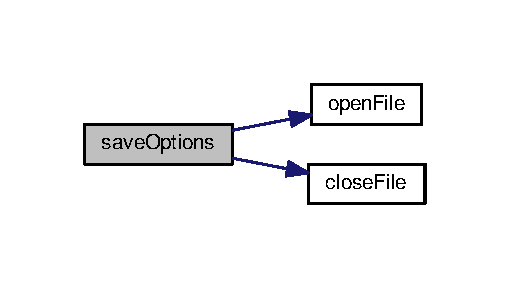
\includegraphics[width=244pt]{option_8h_aa47c7d9be8978d36b12c582b701c534d_cgraph}
\end{center}
\end{figure}



\hypertarget{share_8c}{\subsection{share.\-c File Reference}
\label{share_8c}\index{share.\-c@{share.\-c}}
}


Management of F\-P\-S rate.  


{\ttfamily \#include \char`\"{}share.\-h\char`\"{}}\\*
\subsubsection*{Functions}
\begin{DoxyCompactItemize}
\item 
void \hyperlink{share_8c_a6e428694268169eee69c8f07827e72de}{wait\-F\-P\-S} (int $\ast$previous\-\_\-time, int $\ast$current\-\_\-time)
\end{DoxyCompactItemize}


\subsubsection{Detailed Description}
Management of F\-P\-S rate. \begin{DoxyAuthor}{Author}
Remi B\-E\-R\-T\-H\-O 
\end{DoxyAuthor}
\begin{DoxyDate}{Date}
15/03/14 
\end{DoxyDate}
\begin{DoxyVersion}{Version}
1.\-0 
\end{DoxyVersion}


\subsubsection{Function Documentation}
\hypertarget{share_8c_a6e428694268169eee69c8f07827e72de}{\index{share.\-c@{share.\-c}!wait\-F\-P\-S@{wait\-F\-P\-S}}
\index{wait\-F\-P\-S@{wait\-F\-P\-S}!share.c@{share.\-c}}
\paragraph[{wait\-F\-P\-S}]{\setlength{\rightskip}{0pt plus 5cm}void wait\-F\-P\-S (
\begin{DoxyParamCaption}
\item[{int $\ast$}]{previous\-\_\-time, }
\item[{int $\ast$}]{current\-\_\-time}
\end{DoxyParamCaption}
)}}\label{share_8c_a6e428694268169eee69c8f07827e72de}
Function managing the fps rate 
\begin{DoxyParams}[1]{Parameters}
\mbox{\tt in,out}  & {\em previous\-\_\-time} & The previous time \\
\hline
\mbox{\tt in,out}  & {\em current\-\_\-time} & The current time \\
\hline
\end{DoxyParams}

\hypertarget{share_8h}{\subsection{share.\-h File Reference}
\label{share_8h}\index{share.\-h@{share.\-h}}
}


\hyperlink{share_8c}{share.\-c} header  


{\ttfamily \#include \char`\"{}const.\-h\char`\"{}}\\*
{\ttfamily \#include $<$S\-D\-L/\-S\-D\-L.\-h$>$}\\*
\subsubsection*{Functions}
\begin{DoxyCompactItemize}
\item 
void \hyperlink{share_8h_a6e428694268169eee69c8f07827e72de}{wait\-F\-P\-S} (int $\ast$previous\-\_\-time, int $\ast$current\-\_\-time)
\end{DoxyCompactItemize}


\subsubsection{Detailed Description}
\hyperlink{share_8c}{share.\-c} header \begin{DoxyAuthor}{Author}
Remi B\-E\-R\-T\-H\-O 
\end{DoxyAuthor}
\begin{DoxyDate}{Date}
15/03/14 
\end{DoxyDate}
\begin{DoxyVersion}{Version}
1.\-0 
\end{DoxyVersion}


\subsubsection{Function Documentation}
\hypertarget{share_8h_a6e428694268169eee69c8f07827e72de}{\index{share.\-h@{share.\-h}!wait\-F\-P\-S@{wait\-F\-P\-S}}
\index{wait\-F\-P\-S@{wait\-F\-P\-S}!share.h@{share.\-h}}
\paragraph[{wait\-F\-P\-S}]{\setlength{\rightskip}{0pt plus 5cm}void wait\-F\-P\-S (
\begin{DoxyParamCaption}
\item[{int $\ast$}]{previous\-\_\-time, }
\item[{int $\ast$}]{current\-\_\-time}
\end{DoxyParamCaption}
)}}\label{share_8h_a6e428694268169eee69c8f07827e72de}
Function managing the fps rate 
\begin{DoxyParams}[1]{Parameters}
\mbox{\tt in,out}  & {\em previous\-\_\-time} & The previous time \\
\hline
\mbox{\tt in,out}  & {\em current\-\_\-time} & The current time \\
\hline
\end{DoxyParams}

\hypertarget{text_8c}{\subsection{text.\-c File Reference}
\label{text_8c}\index{text.\-c@{text.\-c}}
}


Management of the display of text on the screen.  


{\ttfamily \#include \char`\"{}text.\-h\char`\"{}}\\*
\subsubsection*{Functions}
\begin{DoxyCompactItemize}
\item 
void \hyperlink{text_8c_a1bd80be1aff6fe5303bdd5aa80161da3}{print\-Text} (S\-D\-L\-\_\-\-Surface $\ast$screen, S\-D\-L\-\_\-\-Rect $\ast$pos\-Text, char $\ast$text, int r, int g, int b, char $\ast$font, int pt\-Size, int mode)
\item 
void \hyperlink{text_8c_abd63f9d237bb4bc462d33c00802cd7b9}{capture\-Text} (S\-D\-L\-\_\-\-Surface $\ast$screen, S\-D\-L\-\_\-\-Rect pos\-Text, char $\ast$text, int text\-\_\-length, int r, int g, int b, char $\ast$font, int text\-\_\-size, int $\ast$go)
\end{DoxyCompactItemize}


\subsubsection{Detailed Description}
Management of the display of text on the screen. \begin{DoxyAuthor}{Author}
Xavier C\-O\-P\-O\-N\-E\-T, Glenn H\-E\-R\-R\-O\-U 
\end{DoxyAuthor}
\begin{DoxyDate}{Date}
2014-\/04-\/27 
\end{DoxyDate}


\subsubsection{Function Documentation}
\hypertarget{text_8c_abd63f9d237bb4bc462d33c00802cd7b9}{\index{text.\-c@{text.\-c}!capture\-Text@{capture\-Text}}
\index{capture\-Text@{capture\-Text}!text.c@{text.\-c}}
\paragraph[{capture\-Text}]{\setlength{\rightskip}{0pt plus 5cm}void capture\-Text (
\begin{DoxyParamCaption}
\item[{S\-D\-L\-\_\-\-Surface $\ast$}]{screen, }
\item[{S\-D\-L\-\_\-\-Rect}]{pos\-Text, }
\item[{char $\ast$}]{text, }
\item[{int}]{text\-\_\-length, }
\item[{int}]{r, }
\item[{int}]{g, }
\item[{int}]{b, }
\item[{char $\ast$}]{font, }
\item[{int}]{text\-\_\-size, }
\item[{int $\ast$}]{go}
\end{DoxyParamCaption}
)}}\label{text_8c_abd63f9d237bb4bc462d33c00802cd7b9}
Capture the text corresponding to the keyboard inputs and display it on the screen at the given position 
\begin{DoxyParams}[1]{Parameters}
\mbox{\tt out}  & {\em screen} & The screen of the game \\
\hline
\mbox{\tt in}  & {\em pos\-Text} & The position of the text. If N\-U\-L\-L, the text is centered \\
\hline
\mbox{\tt out}  & {\em text} & The text to display \\
\hline
\mbox{\tt in}  & {\em r} & red value \\
\hline
\mbox{\tt in}  & {\em g} & green value \\
\hline
\mbox{\tt in}  & {\em b} & blue value \\
\hline
\mbox{\tt in}  & {\em text\-\_\-length} & the text length \\
\hline
\mbox{\tt in}  & {\em font} & The path to the font file \\
\hline
\mbox{\tt in}  & {\em text\-\_\-size} & The text size \\
\hline
\mbox{\tt out}  & {\em go} & The main loop validation \\
\hline
\end{DoxyParams}


Here is the call graph for this function\-:\nopagebreak
\begin{figure}[H]
\begin{center}
\leavevmode
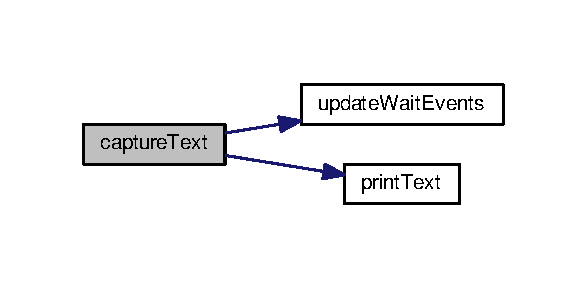
\includegraphics[width=282pt]{text_8c_abd63f9d237bb4bc462d33c00802cd7b9_cgraph}
\end{center}
\end{figure}


\hypertarget{text_8c_a1bd80be1aff6fe5303bdd5aa80161da3}{\index{text.\-c@{text.\-c}!print\-Text@{print\-Text}}
\index{print\-Text@{print\-Text}!text.c@{text.\-c}}
\paragraph[{print\-Text}]{\setlength{\rightskip}{0pt plus 5cm}void print\-Text (
\begin{DoxyParamCaption}
\item[{S\-D\-L\-\_\-\-Surface $\ast$}]{screen, }
\item[{S\-D\-L\-\_\-\-Rect $\ast$}]{pos\-Text, }
\item[{char $\ast$}]{text, }
\item[{int}]{r, }
\item[{int}]{g, }
\item[{int}]{b, }
\item[{char $\ast$}]{font, }
\item[{int}]{pt\-Size, }
\item[{int}]{mode}
\end{DoxyParamCaption}
)}}\label{text_8c_a1bd80be1aff6fe5303bdd5aa80161da3}
Display the given text on the screen, at the given position 
\begin{DoxyParams}[1]{Parameters}
\mbox{\tt out}  & {\em screen} & The screen of the game \\
\hline
\mbox{\tt in}  & {\em pos\-Text} & The position of the text. If N\-U\-L\-L, the text is centered \\
\hline
\mbox{\tt in}  & {\em text} & The text to display \\
\hline
\mbox{\tt in}  & {\em r} & red value \\
\hline
\mbox{\tt in}  & {\em g} & green value \\
\hline
\mbox{\tt in}  & {\em b} & blue value \\
\hline
\mbox{\tt in}  & {\em font} & The path to the font file \\
\hline
\mbox{\tt in}  & {\em pt\-Size} & The text size \\
\hline
\mbox{\tt in}  & {\em mode} & The writing mode \-: 0 (Solid), 1 (Blended) \\
\hline
\end{DoxyParams}

\hypertarget{text_8h}{\subsection{text.\-h File Reference}
\label{text_8h}\index{text.\-h@{text.\-h}}
}


\hyperlink{text_8c}{text.\-c} header  


{\ttfamily \#include $<$stdlib.\-h$>$}\\*
{\ttfamily \#include $<$stdio.\-h$>$}\\*
{\ttfamily \#include $<$errno.\-h$>$}\\*
{\ttfamily \#include \char`\"{}structures.\-h\char`\"{}}\\*
{\ttfamily \#include $<$S\-D\-L/\-S\-D\-L.\-h$>$}\\*
{\ttfamily \#include $<$S\-D\-L/\-S\-D\-L\-\_\-image.\-h$>$}\\*
{\ttfamily \#include $<$S\-D\-L/\-S\-D\-L\-\_\-ttf.\-h$>$}\\*
{\ttfamily \#include \char`\"{}input.\-h\char`\"{}}\\*
\subsubsection*{Functions}
\begin{DoxyCompactItemize}
\item 
void \hyperlink{text_8h_a1bd80be1aff6fe5303bdd5aa80161da3}{print\-Text} (S\-D\-L\-\_\-\-Surface $\ast$screen, S\-D\-L\-\_\-\-Rect $\ast$pos\-Text, char $\ast$text, int r, int g, int b, char $\ast$font, int pt\-Size, int mode)
\item 
void \hyperlink{text_8h_abd63f9d237bb4bc462d33c00802cd7b9}{capture\-Text} (S\-D\-L\-\_\-\-Surface $\ast$screen, S\-D\-L\-\_\-\-Rect pos\-Text, char $\ast$text, int text\-\_\-length, int r, int g, int b, char $\ast$font, int text\-\_\-size, int $\ast$go)
\end{DoxyCompactItemize}


\subsubsection{Detailed Description}
\hyperlink{text_8c}{text.\-c} header \begin{DoxyAuthor}{Author}
Xavier C\-O\-P\-O\-N\-E\-T, Glenn H\-E\-R\-R\-O\-U 
\end{DoxyAuthor}
\begin{DoxyDate}{Date}
2014-\/04-\/27 
\end{DoxyDate}


\subsubsection{Function Documentation}
\hypertarget{text_8h_abd63f9d237bb4bc462d33c00802cd7b9}{\index{text.\-h@{text.\-h}!capture\-Text@{capture\-Text}}
\index{capture\-Text@{capture\-Text}!text.h@{text.\-h}}
\paragraph[{capture\-Text}]{\setlength{\rightskip}{0pt plus 5cm}void capture\-Text (
\begin{DoxyParamCaption}
\item[{S\-D\-L\-\_\-\-Surface $\ast$}]{screen, }
\item[{S\-D\-L\-\_\-\-Rect}]{pos\-Text, }
\item[{char $\ast$}]{text, }
\item[{int}]{text\-\_\-length, }
\item[{int}]{r, }
\item[{int}]{g, }
\item[{int}]{b, }
\item[{char $\ast$}]{font, }
\item[{int}]{text\-\_\-size, }
\item[{int $\ast$}]{go}
\end{DoxyParamCaption}
)}}\label{text_8h_abd63f9d237bb4bc462d33c00802cd7b9}
Capture the text corresponding to the keyboard inputs and display it on the screen at the given position 
\begin{DoxyParams}[1]{Parameters}
\mbox{\tt out}  & {\em screen} & The screen of the game \\
\hline
\mbox{\tt in}  & {\em pos\-Text} & The position of the text. If N\-U\-L\-L, the text is centered \\
\hline
\mbox{\tt out}  & {\em text} & The text to display \\
\hline
\mbox{\tt in}  & {\em r} & red value \\
\hline
\mbox{\tt in}  & {\em g} & green value \\
\hline
\mbox{\tt in}  & {\em b} & blue value \\
\hline
\mbox{\tt in}  & {\em text\-\_\-length} & the text length \\
\hline
\mbox{\tt in}  & {\em font} & The path to the font file \\
\hline
\mbox{\tt in}  & {\em text\-\_\-size} & The text size \\
\hline
\mbox{\tt out}  & {\em go} & The main loop validation \\
\hline
\end{DoxyParams}


Here is the call graph for this function\-:\nopagebreak
\begin{figure}[H]
\begin{center}
\leavevmode
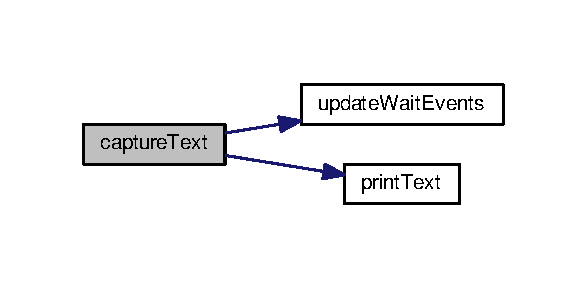
\includegraphics[width=282pt]{text_8h_abd63f9d237bb4bc462d33c00802cd7b9_cgraph}
\end{center}
\end{figure}


\hypertarget{text_8h_a1bd80be1aff6fe5303bdd5aa80161da3}{\index{text.\-h@{text.\-h}!print\-Text@{print\-Text}}
\index{print\-Text@{print\-Text}!text.h@{text.\-h}}
\paragraph[{print\-Text}]{\setlength{\rightskip}{0pt plus 5cm}void print\-Text (
\begin{DoxyParamCaption}
\item[{S\-D\-L\-\_\-\-Surface $\ast$}]{screen, }
\item[{S\-D\-L\-\_\-\-Rect $\ast$}]{pos\-Text, }
\item[{char $\ast$}]{text, }
\item[{int}]{r, }
\item[{int}]{g, }
\item[{int}]{b, }
\item[{char $\ast$}]{font, }
\item[{int}]{pt\-Size, }
\item[{int}]{mode}
\end{DoxyParamCaption}
)}}\label{text_8h_a1bd80be1aff6fe5303bdd5aa80161da3}
Display the given text on the screen, at the given position 
\begin{DoxyParams}[1]{Parameters}
\mbox{\tt out}  & {\em screen} & The screen of the game \\
\hline
\mbox{\tt in}  & {\em pos\-Text} & The position of the text. If N\-U\-L\-L, the text is centered \\
\hline
\mbox{\tt in}  & {\em text} & The text to display \\
\hline
\mbox{\tt in}  & {\em r} & red value \\
\hline
\mbox{\tt in}  & {\em g} & green value \\
\hline
\mbox{\tt in}  & {\em b} & blue value \\
\hline
\mbox{\tt in}  & {\em font} & The path to the font file \\
\hline
\mbox{\tt in}  & {\em pt\-Size} & The text size \\
\hline
\mbox{\tt in}  & {\em mode} & The writing mode \-: 0 (Solid), 1 (Blended) \\
\hline
\end{DoxyParams}

%--- End generated contents ---

% Index
\newpage
\phantomsection
\addcontentsline{toc}{section}{Index}
\printindex

\end{document}
